%\documentclass[letterpaper]{article}
\documentclass[a5paper]{article}

%% Language and font encodings
\usepackage[english]{babel}
\usepackage[utf8x]{inputenc}
\usepackage[T1]{fontenc}

%% Sets page size and margins
%\usepackage[letterpaper,top=1in,bottom=1in,left=1in,right=1in,marginparwidth=1.75cm]{geometry}
\usepackage[a5paper,top=1cm,bottom=1cm,left=1cm,right=1.5cm,marginparwidth=1.75cm]{geometry}
\usepackage{xfrac}


%% Useful packages
\usepackage{amssymb, amsmath, amsthm} 
%\usepackage{graphicx}  %%this is currently enabled in the default document, so it is commented out here. 
\usepackage{calrsfs}
\usepackage{braket}
\usepackage{mathtools}
\usepackage{lipsum}
\usepackage{tikz}
\usetikzlibrary{cd}
\usepackage{verbatim}
%\usepackage{ntheorem}% for theorem-like environments
\usepackage{mdframed}%can make highlighted boxes of text
%Use case: https://tex.stackexchange.com/questions/46828/how-to-highlight-important-parts-with-a-gray-background
\usepackage{wrapfig}
\usepackage{centernot}
\usepackage{subcaption}%\begin{subfigure}{0.5\textwidth}
\usepackage{pgfplots}
\pgfplotsset{compat=1.13}
\usepackage[colorinlistoftodos]{todonotes}
\usepackage[colorlinks=true, allcolors=blue]{hyperref}
\usepackage{xfrac}					%to make slanted fractions \sfrac{numerator}{denominator}
\usepackage{enumitem}            
    %syntax: \begin{enumerate}[label=(\alph*)]
    %possible arguments: f \alph*, \Alph*, \arabic*, \roman* and \Roman*
\usetikzlibrary{arrows,shapes.geometric,fit}

\DeclareMathAlphabet{\pazocal}{OMS}{zplm}{m}{n}
%% Use \pazocal{letter} to typeset a letter in the other kind 
%%  of math calligraphic font. 

%% This puts the QED block at the end of each proof, the way I like it. 
\renewenvironment{proof}{{\bfseries Proof}}{\qed}
\makeatletter
\renewenvironment{proof}[1][\bfseries \proofname]{\par
  \pushQED{\qed}%
  \normalfont \topsep6\p@\@plus6\p@\relax
  \trivlist
  %\itemindent\normalparindent
  \item[\hskip\labelsep
        \scshape
    #1\@addpunct{}]\ignorespaces
}{%
  \popQED\endtrivlist\@endpefalse
}
\makeatother

%% This adds a \rewnewtheorem command, which enables me to override the settings for theorems contained in this document.
\makeatletter
\def\renewtheorem#1{%
  \expandafter\let\csname#1\endcsname\relax
  \expandafter\let\csname c@#1\endcsname\relax
  \gdef\renewtheorem@envname{#1}
  \renewtheorem@secpar
}
\def\renewtheorem@secpar{\@ifnextchar[{\renewtheorem@numberedlike}{\renewtheorem@nonumberedlike}}
\def\renewtheorem@numberedlike[#1]#2{\newtheorem{\renewtheorem@envname}[#1]{#2}}
\def\renewtheorem@nonumberedlike#1{  
\def\renewtheorem@caption{#1}
\edef\renewtheorem@nowithin{\noexpand\newtheorem{\renewtheorem@envname}{\renewtheorem@caption}}
\renewtheorem@thirdpar
}
\def\renewtheorem@thirdpar{\@ifnextchar[{\renewtheorem@within}{\renewtheorem@nowithin}}
\def\renewtheorem@within[#1]{\renewtheorem@nowithin[#1]}
\makeatother

%% This makes theorems and definitions with names show up in bold, the way I like it. 
\makeatletter
\def\th@plain{%
  \thm@notefont{}% same as heading font
  \itshape % body font
}
\def\th@definition{%
  \thm@notefont{}% same as heading font
  \normalfont % body font
}
\makeatother

%===============================================
%==============Shortcut Commands================
%===============================================
\newcommand{\ds}{\displaystyle}
\newcommand{\B}{\mathcal{B}}
\newcommand{\C}{\mathbb{C}}
\newcommand{\F}{\mathbb{F}}
\newcommand{\N}{\mathbb{N}}
\newcommand{\R}{\mathbb{R}}
\newcommand{\Q}{\mathbb{Q}}
\newcommand{\T}{\mathcal{T}}
\newcommand{\Z}{\mathbb{Z}}
\renewcommand\qedsymbol{$\blacksquare$}
\newcommand{\qedwhite}{\hfill\ensuremath{\square}}
\newcommand*\conj[1]{\overline{#1}}
\newcommand*\closure[1]{\overline{#1}}
\newcommand*\mean[1]{\overline{#1}}
%\newcommand{\inner}[1]{\left< #1 \right>}
\newcommand{\inner}[2]{\left< #1, #2 \right>}
\newcommand{\powerset}[1]{\pazocal{P}(#1)}
%% Use \pazocal{letter} to typeset a letter in the other kind 
%%  of math calligraphic font. 
\newcommand{\cardinality}[1]{\left| #1 \right|}
\newcommand{\domain}[1]{\mathcal{D}(#1)}
\newcommand{\image}{\text{Im}}
\newcommand{\inv}[1]{#1^{-1}}
\newcommand{\preimage}[2]{#1^{-1}\left(#2\right)}
\newcommand{\script}[1]{\mathcal{#1}}


\newenvironment{highlight}{\begin{mdframed}[backgroundcolor=gray!20]}{\end{mdframed}}

\DeclarePairedDelimiter\ceil{\lceil}{\rceil}
\DeclarePairedDelimiter\floor{\lfloor}{\rfloor}

%===============================================
%===============My Tikz Commands================
%===============================================
\newcommand{\drawsquiggle}[1]{\draw[shift={(#1,0)}] (.005,.05) -- (-.005,.02) -- (.005,-.02) -- (-.005,-.05);}
\newcommand{\drawpoint}[2]{\draw[*-*] (#1,0.01) node[below, shift={(0,-.2)}] {#2};}
\newcommand{\drawopoint}[2]{\draw[o-o] (#1,0.01) node[below, shift={(0,-.2)}] {#2};}
\newcommand{\drawlpoint}[2]{\draw (#1,0.02) -- (#1,-0.02) node[below] {#2};}
\newcommand{\drawlbrack}[2]{\draw (#1+.01,0.02) --(#1,0.02) -- (#1,-0.02) -- (#1+.01,-0.02) node[below, shift={(-.01,0)}] {#2};}
\newcommand{\drawrbrack}[2]{\draw (#1-.01,0.02) --(#1,0.02) -- (#1,-0.02) -- (#1-.01,-0.02) node[below, shift={(+.01,0)}] {#2};}

%***********************************************
%**************Start of Document****************
%***********************************************
 %find me at /home/trevor/texmf/tex/latex/tskpreamble_nothms.tex
%\newcommand{\curl}{\text{curl}}


\graphicspath{{/home/trevor/Documents/latex/images/}{/home/trevor/Documents/latex/images/adv_calc/}}

%===============================================
%===============Theorem Styles==================
%===============================================

%================Default Style==================
%\theoremstyle{plain}% is the default. it sets the text in italic and adds extra space above and below the \newtheorems listed below it in the input. it is recommended for theorems, corollaries, lemmas, propositions, conjectures, criteria, and (possibly; depends on the subject area) algorithms.
%===============Highlight Style=================
\usepackage{xcolor}
\usepackage{mdframed}
%\newtheorem{mdtheorem}{Theorem}
\newenvironment{theorembold}%
  {\begin{mdframed}[backgroundcolor=gray!20]\begin{mdtheorem}}%
  {\end{mdtheorem}\end{mdframed}}
  
%\begin{comment}
%==============Definition Style=================
\theoremstyle{definition}% adds extra space above and below, but sets the text in roman. it is recommended for definitions, conditions, problems, and examples; i've alse seen it used for exercises.
\newtheorem{theorem}{Theorem}
%\numberwithin{theorem}{section} %This sets the numbering system for theorems to number them down to the {argument} level. I have it set to number down to the {section} level right now.
\newtheorem*{theorem*}{Theorem} %Theorem with no numbering
\newtheorem{corollary}[theorem]{Corollary}
\newtheorem*{corollary*}{Corollary}
\newtheorem{conjecture}[theorem]{Conjecture}
\newtheorem{lemma}[theorem]{Lemma}
\newtheorem*{lemma*}{Lemma}
\newtheorem{proposition}[theorem]{Proposition}
\newtheorem*{proposition*}{Proposition}
\newtheorem{problemstatement}[theorem]{Problem Statement}

\newtheorem{definition}[theorem]{Definition}
\newtheorem*{definition*}{Definition}
\newtheorem{condition}[theorem]{Condition}
\newtheorem{problem}[theorem]{Problem}
\newtheorem{example}[theorem]{Example}
\newtheorem*{example*}{Example}
\newtheorem*{romantheorem*}{Theorem} %Theorem with no numbering
\newtheorem{exercise}{Exercise}
\numberwithin{exercise}{section}
\newtheorem{algorithm}[theorem]{Algorithm}

%================Remark Style===================
\theoremstyle{remark}% is set in roman, with no additional space above or below. it is recommended for remarks, notes, notation, claims, summaries, acknowledgments, cases, and conclusions.
\newtheorem{remark}[theorem]{Remark}
\newtheorem*{remark*}{Remark}
\newtheorem{notation}[theorem]{Notation}
%\newtheorem{claim}[theorem]{Claim}  %%use this if you ever want claims to be numbered
\newtheorem*{claim}{Claim}
%\end{comment}

%===============================================
%===========Document-specific commands==========
%===============================================
%\newcommand{\T}{\mathcal{T}}
%\newcommand{\B}{\mathcal{B}}
%\newcommand{\S}{\mathcal{S}}

%These commands are now in tskpreamble_nothms.tex, but are left as a comment here for reference. 
%\newcommand{\arbcup}[1]{\bigcup\limits_{\alpha\in\Gamma}#1_\alpha}
%\newcommand{\arbcap}[1]{\bigcap\limits_{\alpha\in\Gamma}#1_\alpha}
%\newcommand{\arbcoll}[1]{\{#1_\alpha\}_{\alpha\in\Gamma}}
%\newcommand{\arbprod}[1]{\prod\limits_{\alpha\in\Gamma}#1_\alpha}
%\newcommand{\finitecoll}[1]{#1_1, \ldots, #1_n}
%\newcommand{\finitefuncts}[2]{#1(#2_1), \ldots, #1(#2_n)}
%\newcommand{\abs}[1]{\left|#1\right|}
%\newcommand{\norm}[1]{\left|\left|#1\right|\right|}


%================Start of document==============

\title{Advanced Calculus II - Fuller, 2018}
\author{Trevor Klar}
\makeindex

\begin{document}
\maketitle

\tableofcontents

\addcontentsline{toc}{section}{Introduction}

%\begin{mdframed}[backgroundcolor=blue!20]
%If you would like to copy and paste some of this \LaTeX \, for your own notes, you can download the .tex file \href{https://goo.gl/GYnmeX}{here}. (Warning, this file won't compile as-is, it needs a bunch of other files which are stored on my computer.)
%\end{mdframed}

\begin{highlight}
Note: If you find any typos in these notes, please let me know at \\ \href{mailto:trevor.klar.834@my.csun.edu}{trevor.klar.834@my.csun.edu}. If you could include the page number, that would be helpful. 

Note to the reader: I have highlighted topics which seem important to me, but the emphasis is mine, not Professor Fuller's. Bear that in mind when studying. 
\end{highlight}

\pagebreak
\section{Introduction}

Advanced Calculus I, is analysis, differentiation, integration and so on of functions of one variable. This class, Advanced Calculus II, deals with many of the same concepts, but with \emph{multivariable} functions. 

\subsection{Basic Definitions}

You should know these definitions, but in case you don't, or need a specific reference, here they are. 

\begin{definition*}
$\R^n=\{(x_1, \ldots, x_n):x_i\in \R\}.$
\end{definition*}

Notation: $\vecb{x}=(x_1, \ldots, x_n)$

\begin{center}
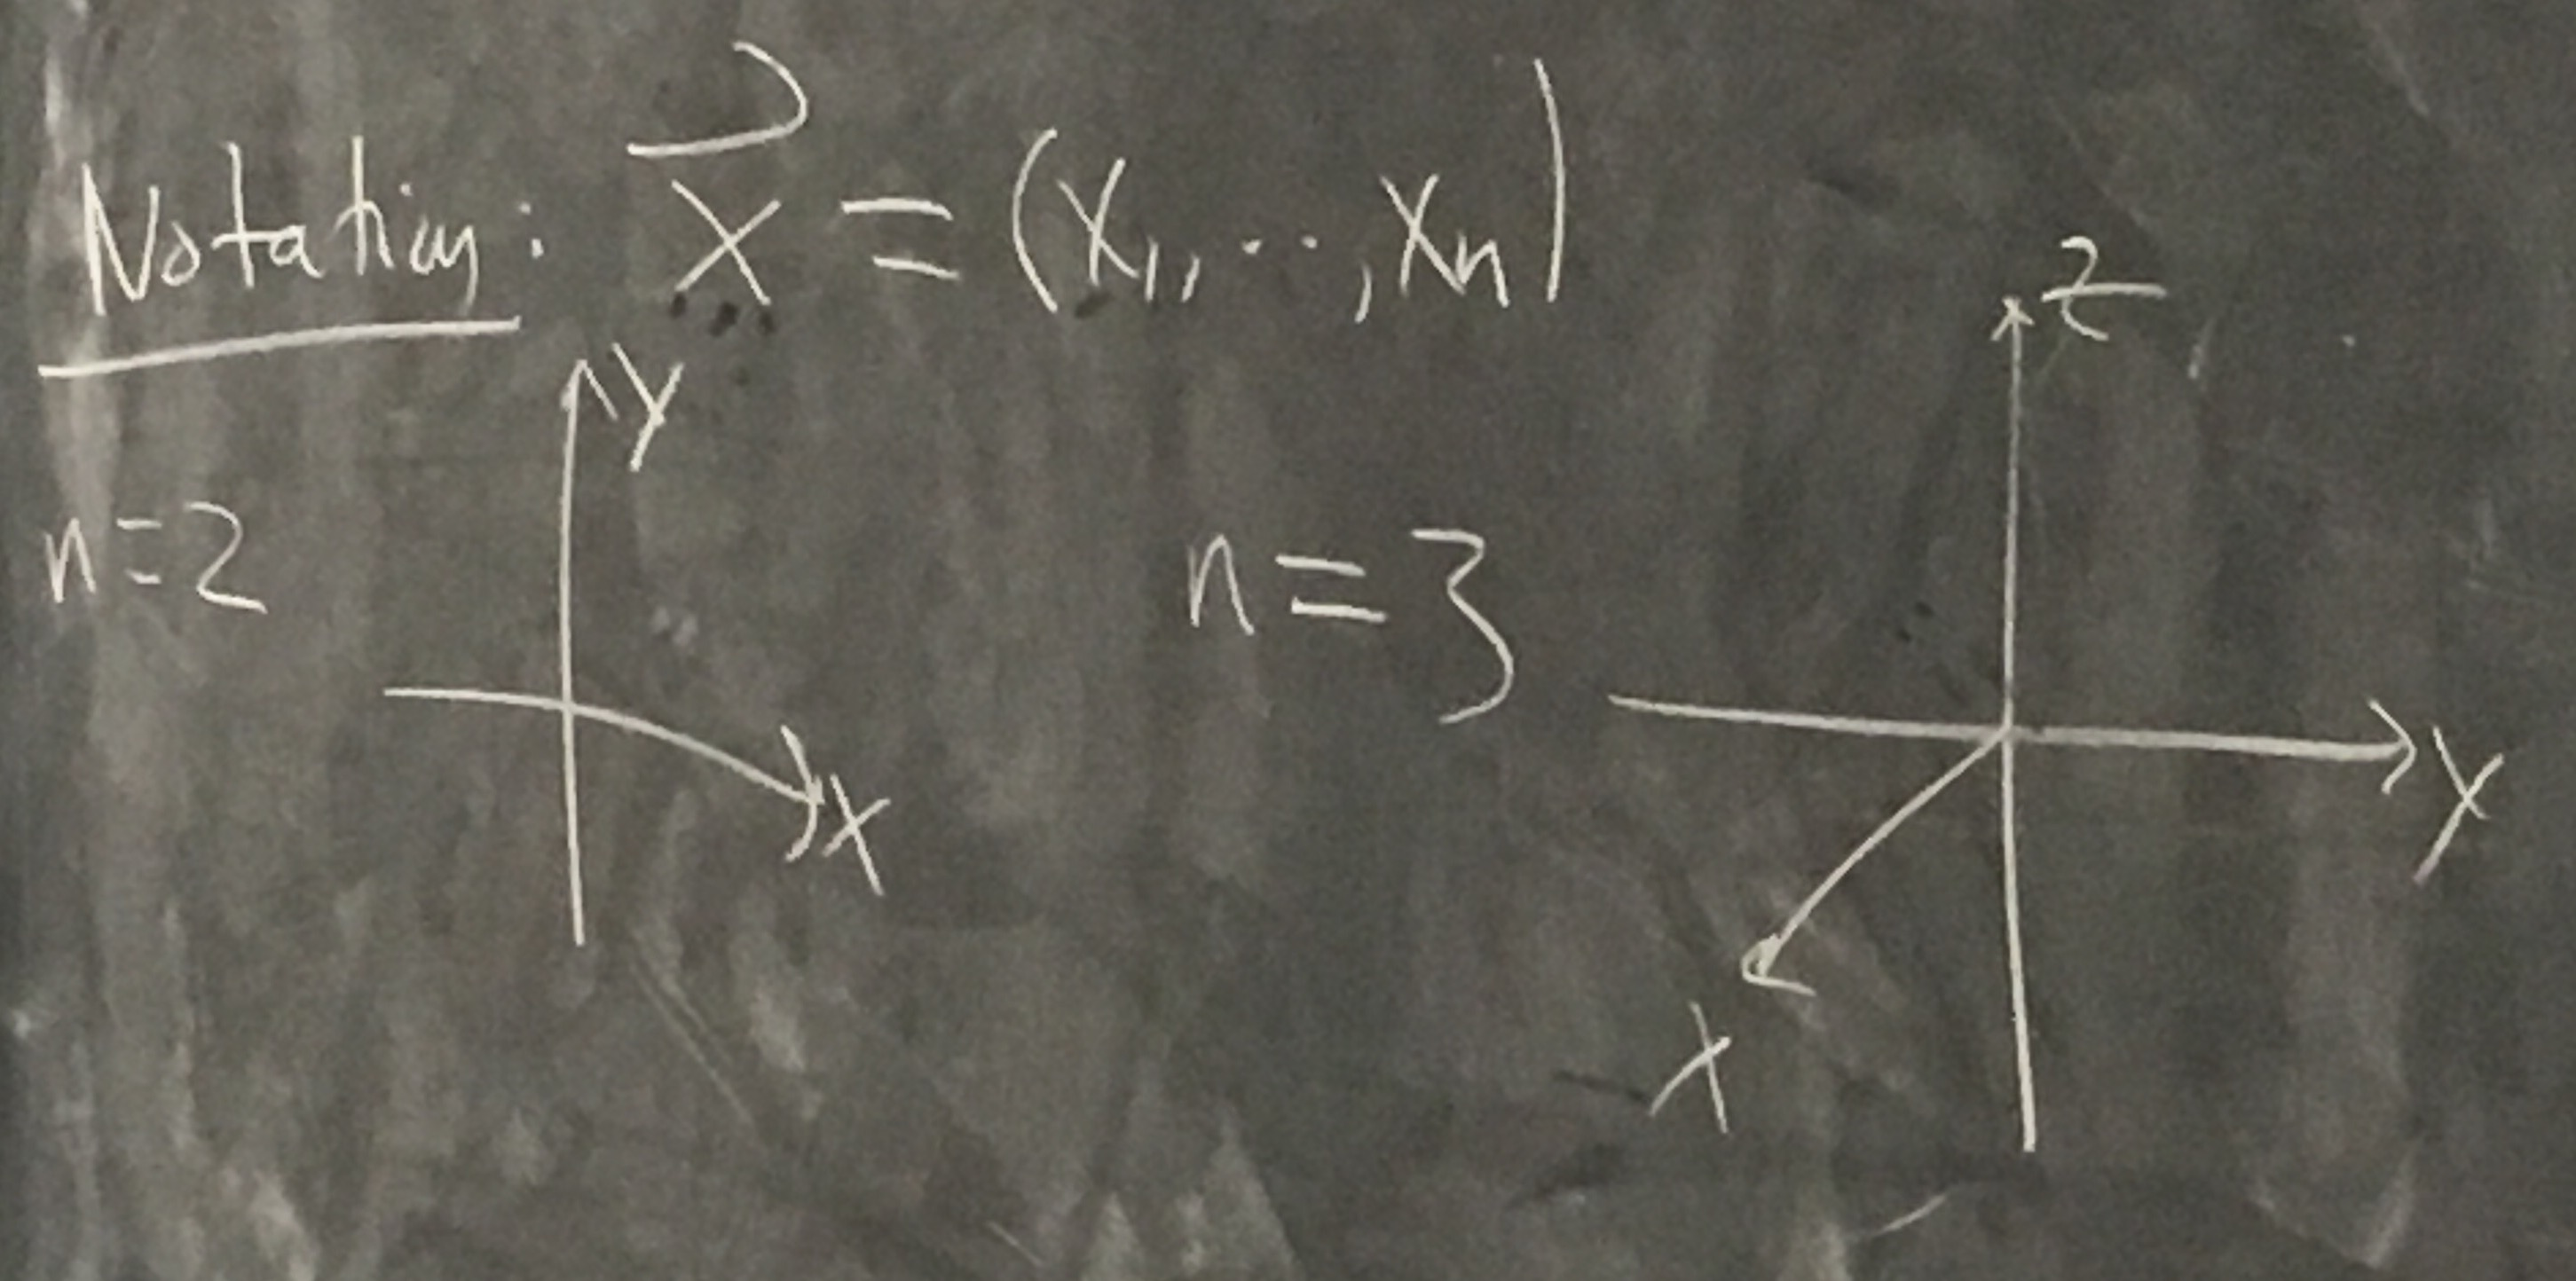
\includegraphics[scale=.07]{definitions_1}
\end{center}

We will add and scalar multiply vectors as in the usual vector space structure on $\R^n$. (i.e. addition and scalar multiplication are as you would expect.)

\begin{definition*}
We find the \emph{absolute value} \index{absolute value} (or \emph{norm}) of a vector as usual, that is:

$$\norm{\vecb{x}}=(\sum x_i^2)^{\frac{1}{2}}$$
\end{definition*}

\begin{definition*}
We find distance between vectors also as usual:

$$\norm{\vecb{x}-\vecb{y}}=(\sum(x_i-y_i)^2)^{\frac{1}{2}}$$

We may sometimes use the folowing notation as shorthand for the same thing. 

$$d(\vecb{x},\vecb{y})=\norm{\vecb{x}-\vecb{y}}$$
\end{definition*}

\begin{definition*}
We use the following inner product (sometimes called the \emph{dot product}):

Given $\vecb{x} \vecb{y}, \in \R^n$, 

$$\inner{\vecb{x}} {\vecb{y}}=\sum_{i=1}^n x_i y_i$$

\end{definition*}

\pagebreak
\begin{proposition}
For all $\vecb{x} \vecb{y}, \vecb{z}, \in \R^n$, and all $r \in \R$:

\begin{enumerate}
%(start numbering at 0)
\setcounter{enumi}{-1}
\item $\inner{\vecb{x}}{\vecb{x}}=\norm{\vecb{x}}^2$
\item $\norm{\vecb{x}}\geq0$, and $\norm{\vecb{x}}=0$ if and only if $\vecb{x}=\vecb{0}$ (norm is positive definite)
\item $\norm{r\vecb{x}}=\abs{r}\norm{\vecb{x}}$
\item \quad \begin{highlight}
$\norm{\vecb{x}+\vecb{y}}\leq\norm{\vecb{x}}+\norm{\vecb{y}}$ (The Triangle Inequality)
\end{highlight}
\item $\inner{\vecb{x}}{\vecb{x}} \geq 0$, and $\inner{\vecb{x}}{\vecb{x}}=0$  if and only if $\vecb{x}=\vecb{0}$ (distance is positive definite)
\item $\inner{\vecb{x}}{\vecb{y}+\vecb{z}}=\inner{\vecb{x}}{\vecb{y}}+\inner{\vecb{x}}{\vecb{z}}$ (Left distributive property)
\item $\inner{r\vecb{x}}{\vecb{y}}=r\inner{\vecb{x}}{\vecb{y}}$
\item $\inner{\vecb{x}}{\vecb{y}}=\inner{\vecb{y}}{\vecb{x}}$ (commutative)
\end{enumerate}
The proofs for all these except (3) follow immediately from definitions. 
\end{proposition}

\begin{remark*}\mbox{}\\
\begin{itemize}
\item(5)+(7) imply $\inner{\vecb{x}+\vecb{y}}{\vecb{z}}=\inner{\vecb{x}}{\vecb{z}}+\inner{\vecb{y}}{\vecb{z}}$. \\
\item(6)+(7) imply $\inner{\vecb{x}}{r\vecb{y}}=r\inner{\vecb{x}}{\vecb{y}}$. \\
\item(3) implies the Reverse Triangle Inequality:
$$\abs{\,\norm{\vecb{x}}-\norm{\vecb{y}}\,}\leq\norm{\vecb{x}-\vecb{y}}$$
\begin{proof}
(proof in image)
\end{proof}

\item Also, $\inner{x+y}{z_w}$ can be "foil"ed the way you expect. 

\end{itemize}
\end{remark*}

\subsection{Geometric interpretation of Inner Product}

\begin{center}
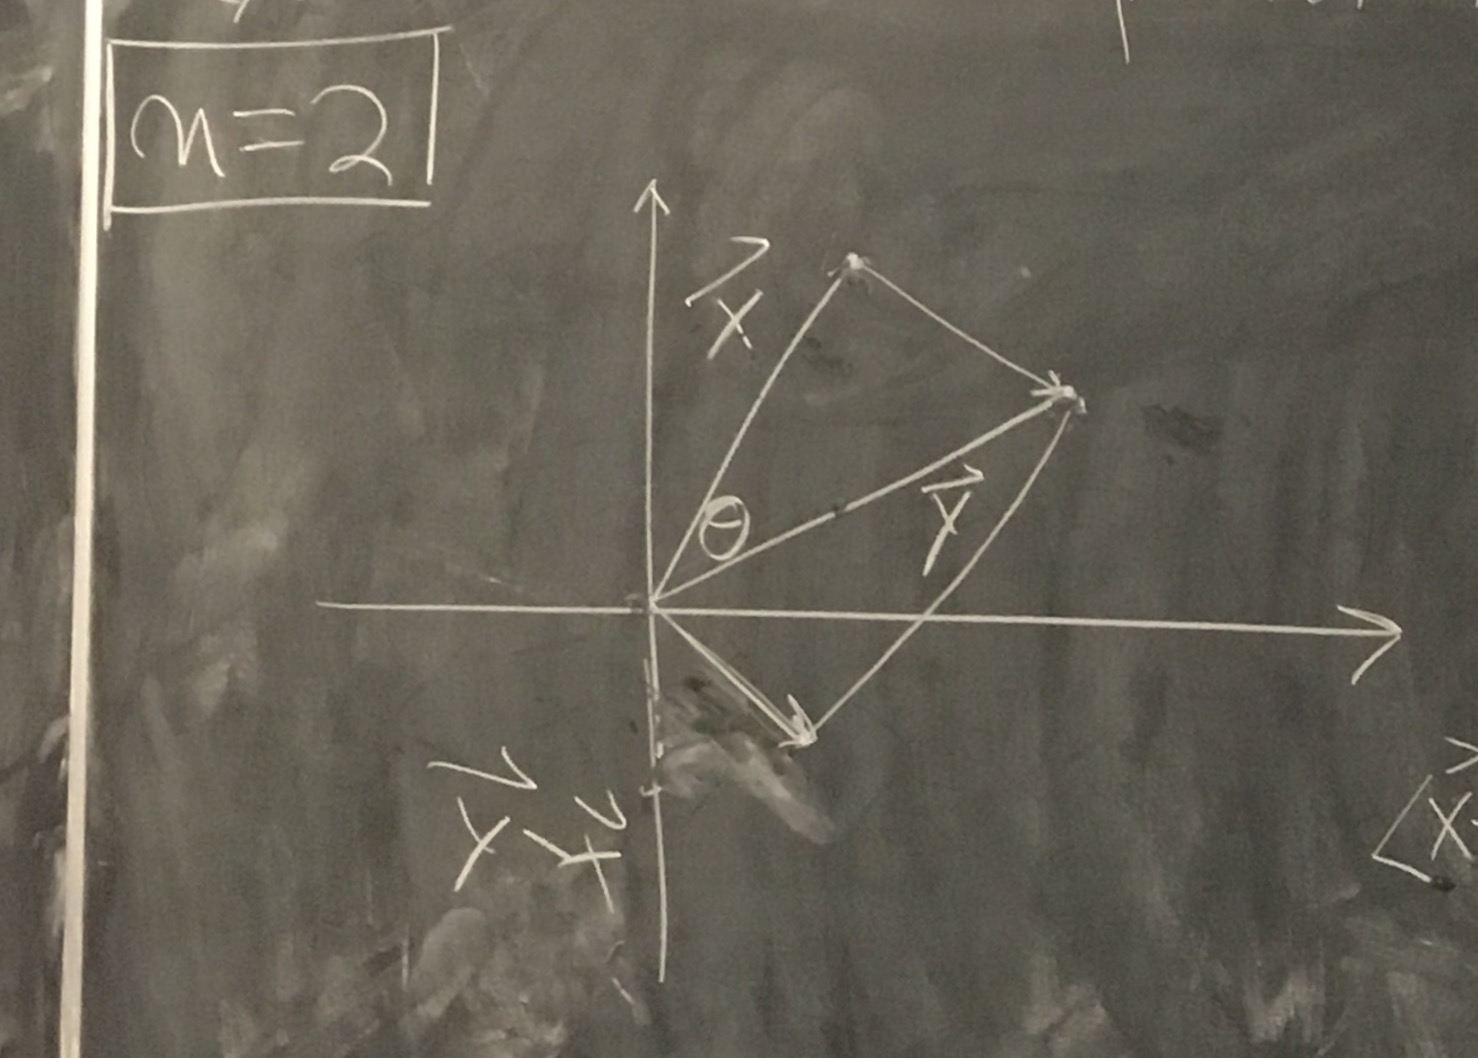
\includegraphics[scale=.12]{geometric_inner_1}
\end{center}

Consider the two vectors $\vecb{x}$ and $\vecb{y}$ above which, together with $\vecb{x}=\vecb{y}$, form a triangle. Now, by the Law of Cosines:
$$\norm{\vecb{x}-\vecb{y}}^2=\norm{\vecb{x}}^2+\norm{\vecb{y}}^2-2\norm{\vecb{x}}\norm{\vecb{y}}\cos\theta.$$
Also, by applying Prop 1.0, 
$$\norm{\vecb{x}-\vecb{y}}^2=\inner{\vecb{x}-\vecb{y}}{\vecb{x}-\vecb{y}}=\norm{\vecb{x}}^2+\norm{\vecb{y}}^2-2\inner{\vecb{x}}{\vecb{y}}.$$

This implies 
$$\cos\theta=\frac{\inner{\vecb{x}}{\vecb{y}}}{\norm{\vecb{x}}\norm{\vecb{y}}}.$$
(If you're not convinced, equate the RHS's of the above equations and solve for $\cos\theta$.)

This leads us to the following definition:

\begin{highlight}
\begin{definition*}
Given $\vecb{x}, \vecb{y}\in \R^n$, we define the angle between $\vecb{x}$ and $\vecb{y}$ as the angle $\theta\in[0,\pi]$ with $\cos\theta=\frac{\inner{\vecb{x}}{\vecb{y}}}{\norm{\vecb{x}}\norm{\vecb{y}}}$.
\end{definition*}
\end{highlight}

\begin{definition*}
We say that $\vecb{x}$ and $\vecb{y}$ are \emph{parallel} if and only if $\theta=0$. 
We say that $\vecb{x}$ and $\vecb{y}$ are \emph{orthogonal} if and only if $\theta=\frac{\pi}{2}$. 
\end{definition*}

Facts: 
\begin{itemize}
\item $\vecb{x}$ and $\vecb{y}$ are parallel if and only if $\vecb{x}=r\vecb{y}$ with $r>0$ (the proof is an excercise). 
\item $\vecb{x}$ and $\vecb{y}$ are orthogonal if and only if $\inner{\vecb{x}}{\vecb{y}}=0$. 
\end{itemize}

\begin{highlight}
\begin{proposition}(Cauchy-Schwarz Inequality)
For all $\vecb{x}, \vecb{y}, \in \R$, 
$$\abs{\inner{\vecb{x}}{\vecb{y}}}\leq \norm{\vecb{x}}\norm{\vecb{y}}$$
\end{proposition}
\end{highlight}
\begin{proof}
For all $r\in\R$, 
\[\begin{array}{rcl}
0&\leq&\norm{\vecb{x}-r\vecb{y}}^2\\
&=&\norm{\vecb{x}}^2-2r\inner{\vecb{x}}{\vecb{y}}+r^2\norm{\vecb{y}}^2.
\end{array}\]

Now since this inequality holds for every $r$, let $r=\frac{\inner{\vecb{x}}{\vecb{y}}}{\norm{\vecb{y}}^2}$. Then, 
\[\begin{array}{rcl}
0&\leq&\norm{\vecb{x}}^2-2\frac{\inner{\vecb{x}}{\vecb{y}}}{\norm{\vecb{y}}^2}\inner{\vecb{x}}{\vecb{y}}+\frac{\inner{\vecb{x}}{\vecb{y}}^2}{\norm{\vecb{y}}^4}\norm{\vecb{y}}^2.\\
&=&\norm{\vecb{x}}^2-2\frac{\inner{\vecb{x}}{\vecb{y}}^2}{\norm{\vecb{y}}^2}+\frac{\inner{\vecb{x}}{\vecb{y}}^2}{\norm{\vecb{y}}^2}.\\
&=&\norm{\vecb{x}}^2-\frac{\inner{\vecb{x}}{\vecb{y}}^2}{\norm{\vecb{y}}^2}.
\end{array}\]

Thus, we can see that $\inner{\vecb{x}}{\vecb{y}}^2\leq\norm{\vecb{x}}^2\norm{\vecb{y}}^2$, and, taking square roots, wee obtain $\left|\inner{\vecb{x}}{\vecb{y}}\right|\leq\norm{\vecb{x}}\norm{\vecb{y}}$ and we are done. 
\end{proof}

\begin{proof}
%%%%%%%%%%%%%%%%%%%%%%%%%%%%%%%%%%%%%%%%%%%%%%%%%%%%%%%%%%%%%%
%FIX THIS 
%%%%%%%%%%%%%%%%%%%%%%%%%%%%%%%%%%%%%%%%%%%%%%%%%%%%%%%%%%%%%%
%$$\norm{\vecb{x}+\vecb{y}}^2=\norm{\vecb{x}}^2+2\inner{\vecb{x}}{\vecb{y}}+\norm{\vecb{y}}^2\leq\norm{\vecb{x}}^2+2\norm{\vecb{x}}\norm{\vecb{y}}+\norm{\vecb{y}}^2\=(\norm{\vecb{x}}+\norm{\vecb{y}})^2$$
This implies the triangle inequality. 
\end{proof}

\subsection{Open Balls and Open Sets}
\begin{highlight}
\begin{definition*}
Given $\vecb{x_0}\in\R^n$, $r>0$: We say that a \emph{ball of radius $r$ centered at $x_0$} is 
$$B(\vecb{x_0}, r)=\{\vecb{x}:\norm{\vecb{x}-\vecb{x_0}}<r\}.$$
\end{definition*}
\end{highlight}

\begin{highlight}
\begin{definition*}
A subset $U\subseteq \R^n$ is \emph{open in $R^n$} if for every $\vecb{x}\in U$, there is $r>0$ such that $B(\vecb{x_0}, r) \subseteq U $. 
\end{definition*}
\end{highlight}

\begin{example*}
\begin{enumerate}\mbox{}

\item $(a,b)\subseteq\R^1$ is open in $\R$.
\begin{center}
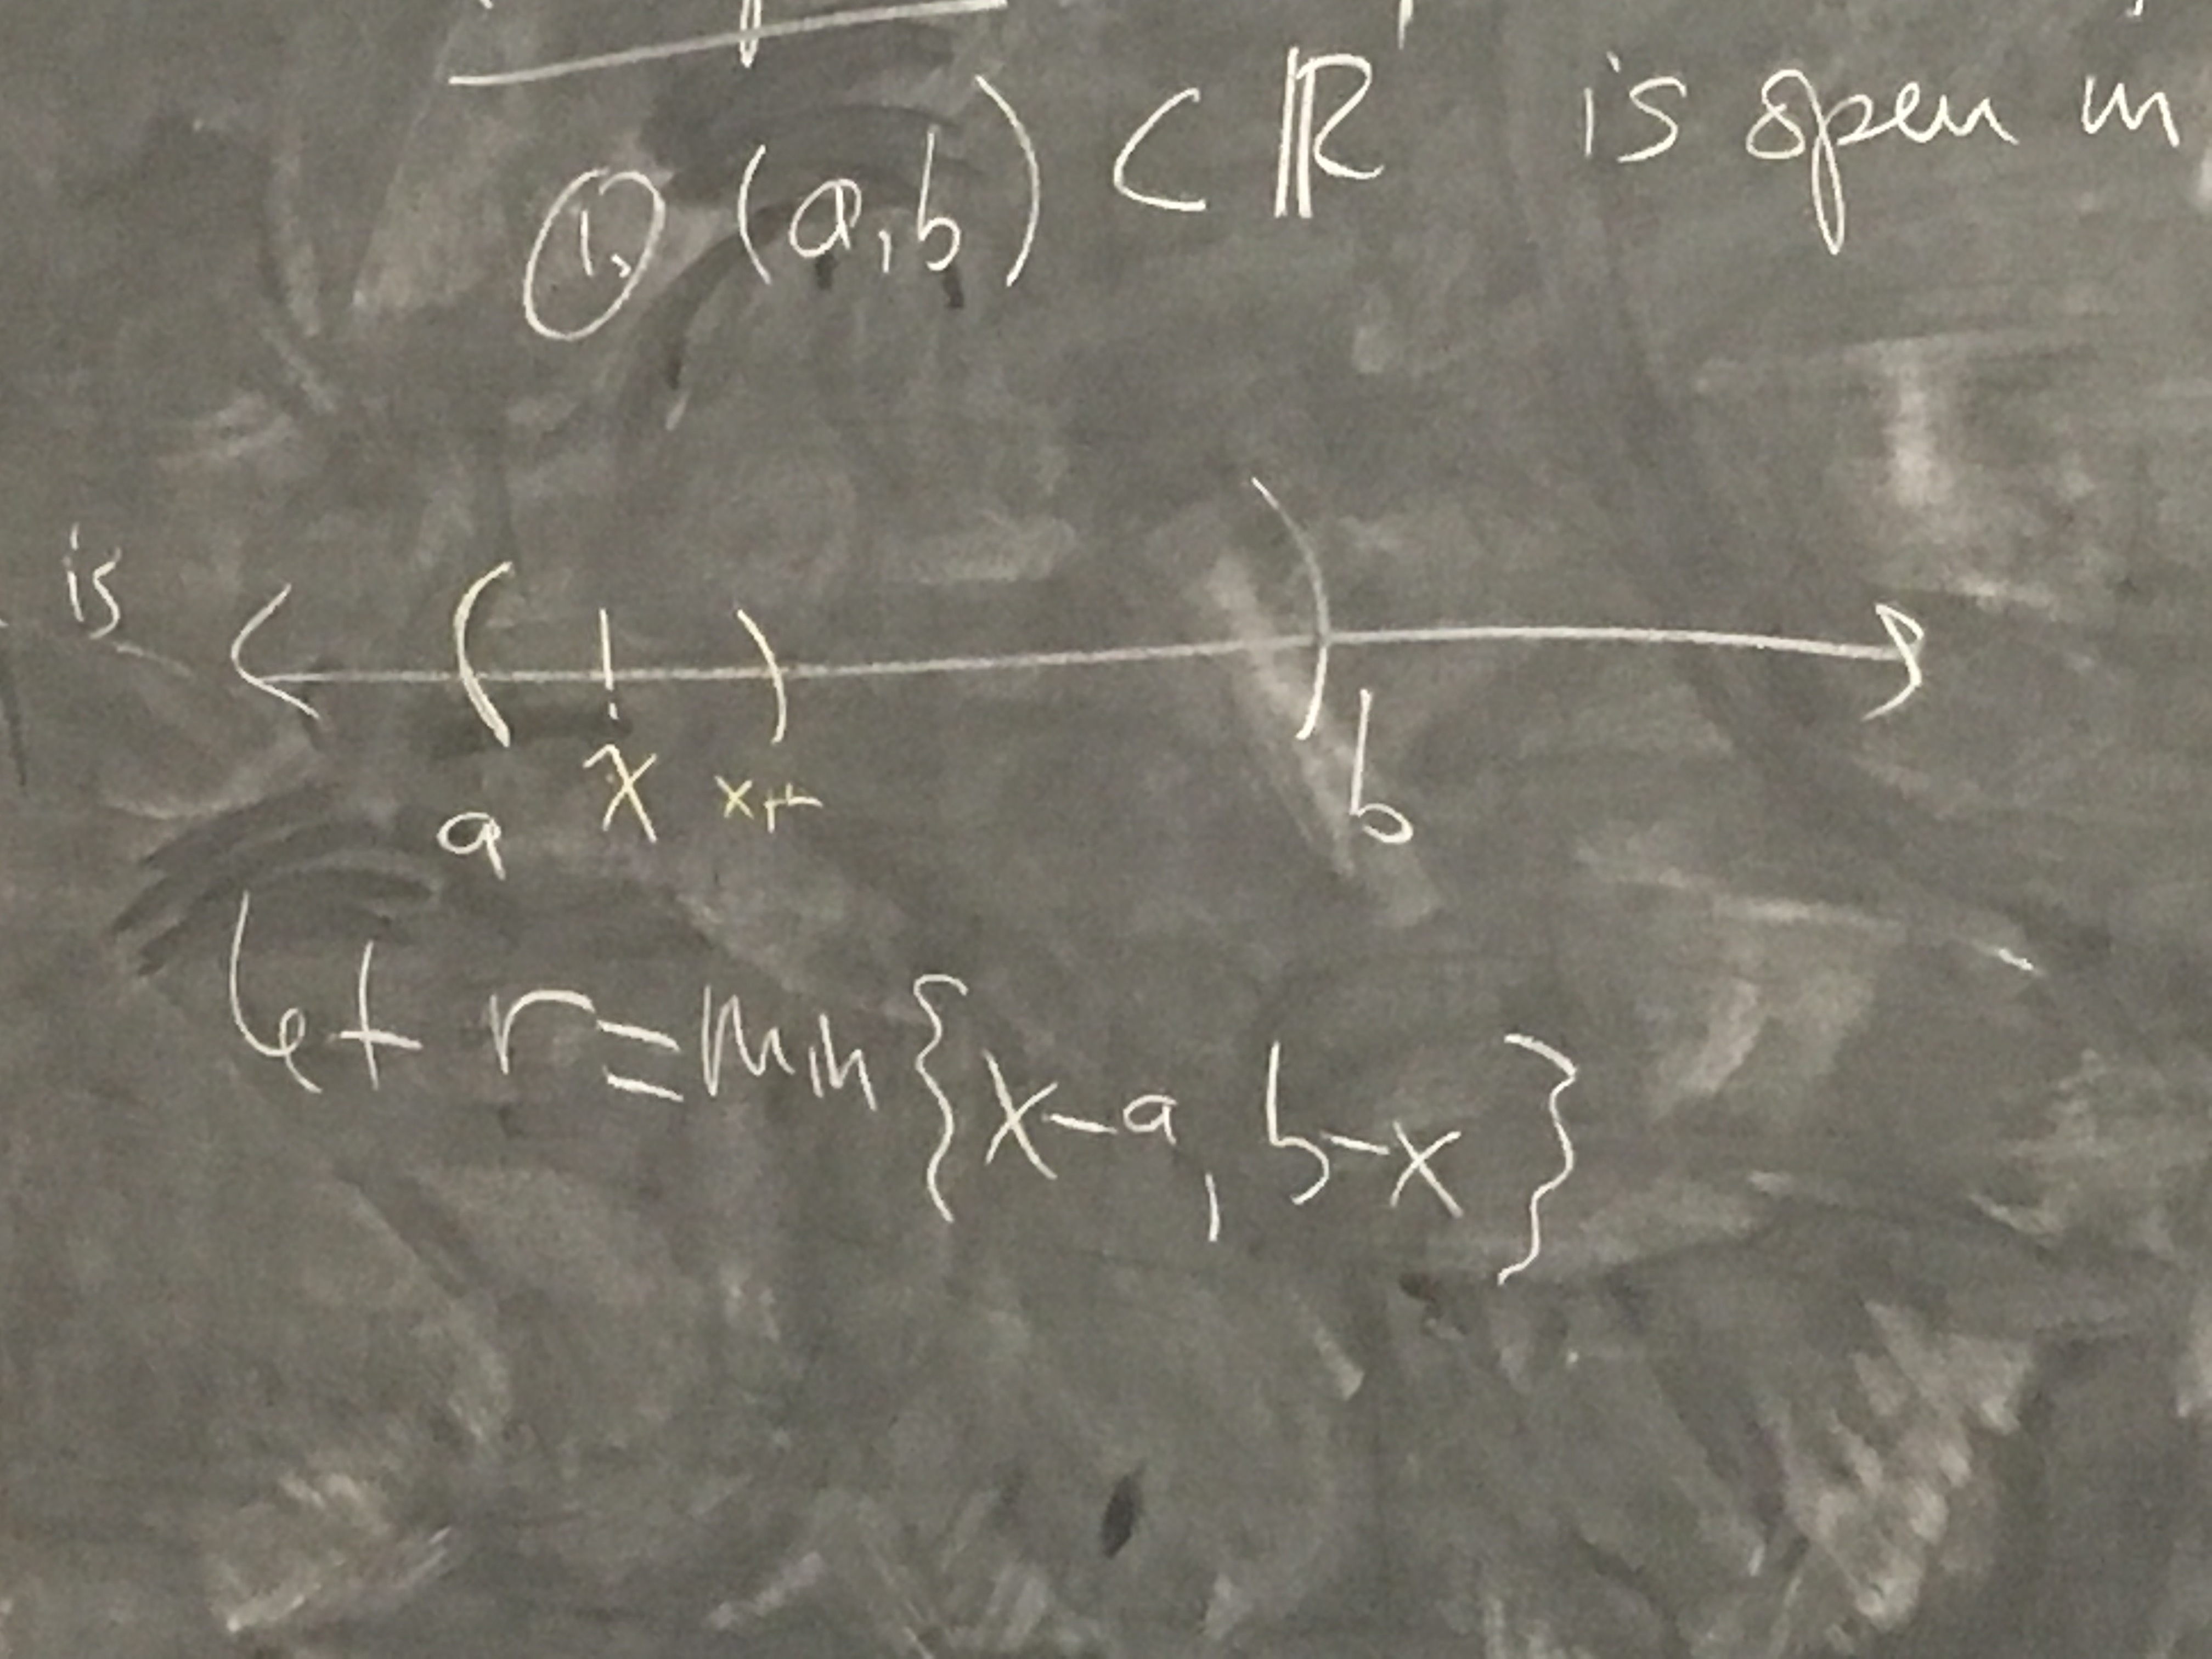
\includegraphics[scale=.05]{open_balls_1}
\end{center}

\item Let $(a,b)\times\{0\}=\{(x,y):a<x<b, y=0\}\subset \R^2$. This set is \emph{not} open in $R^2$. 
\begin{center}
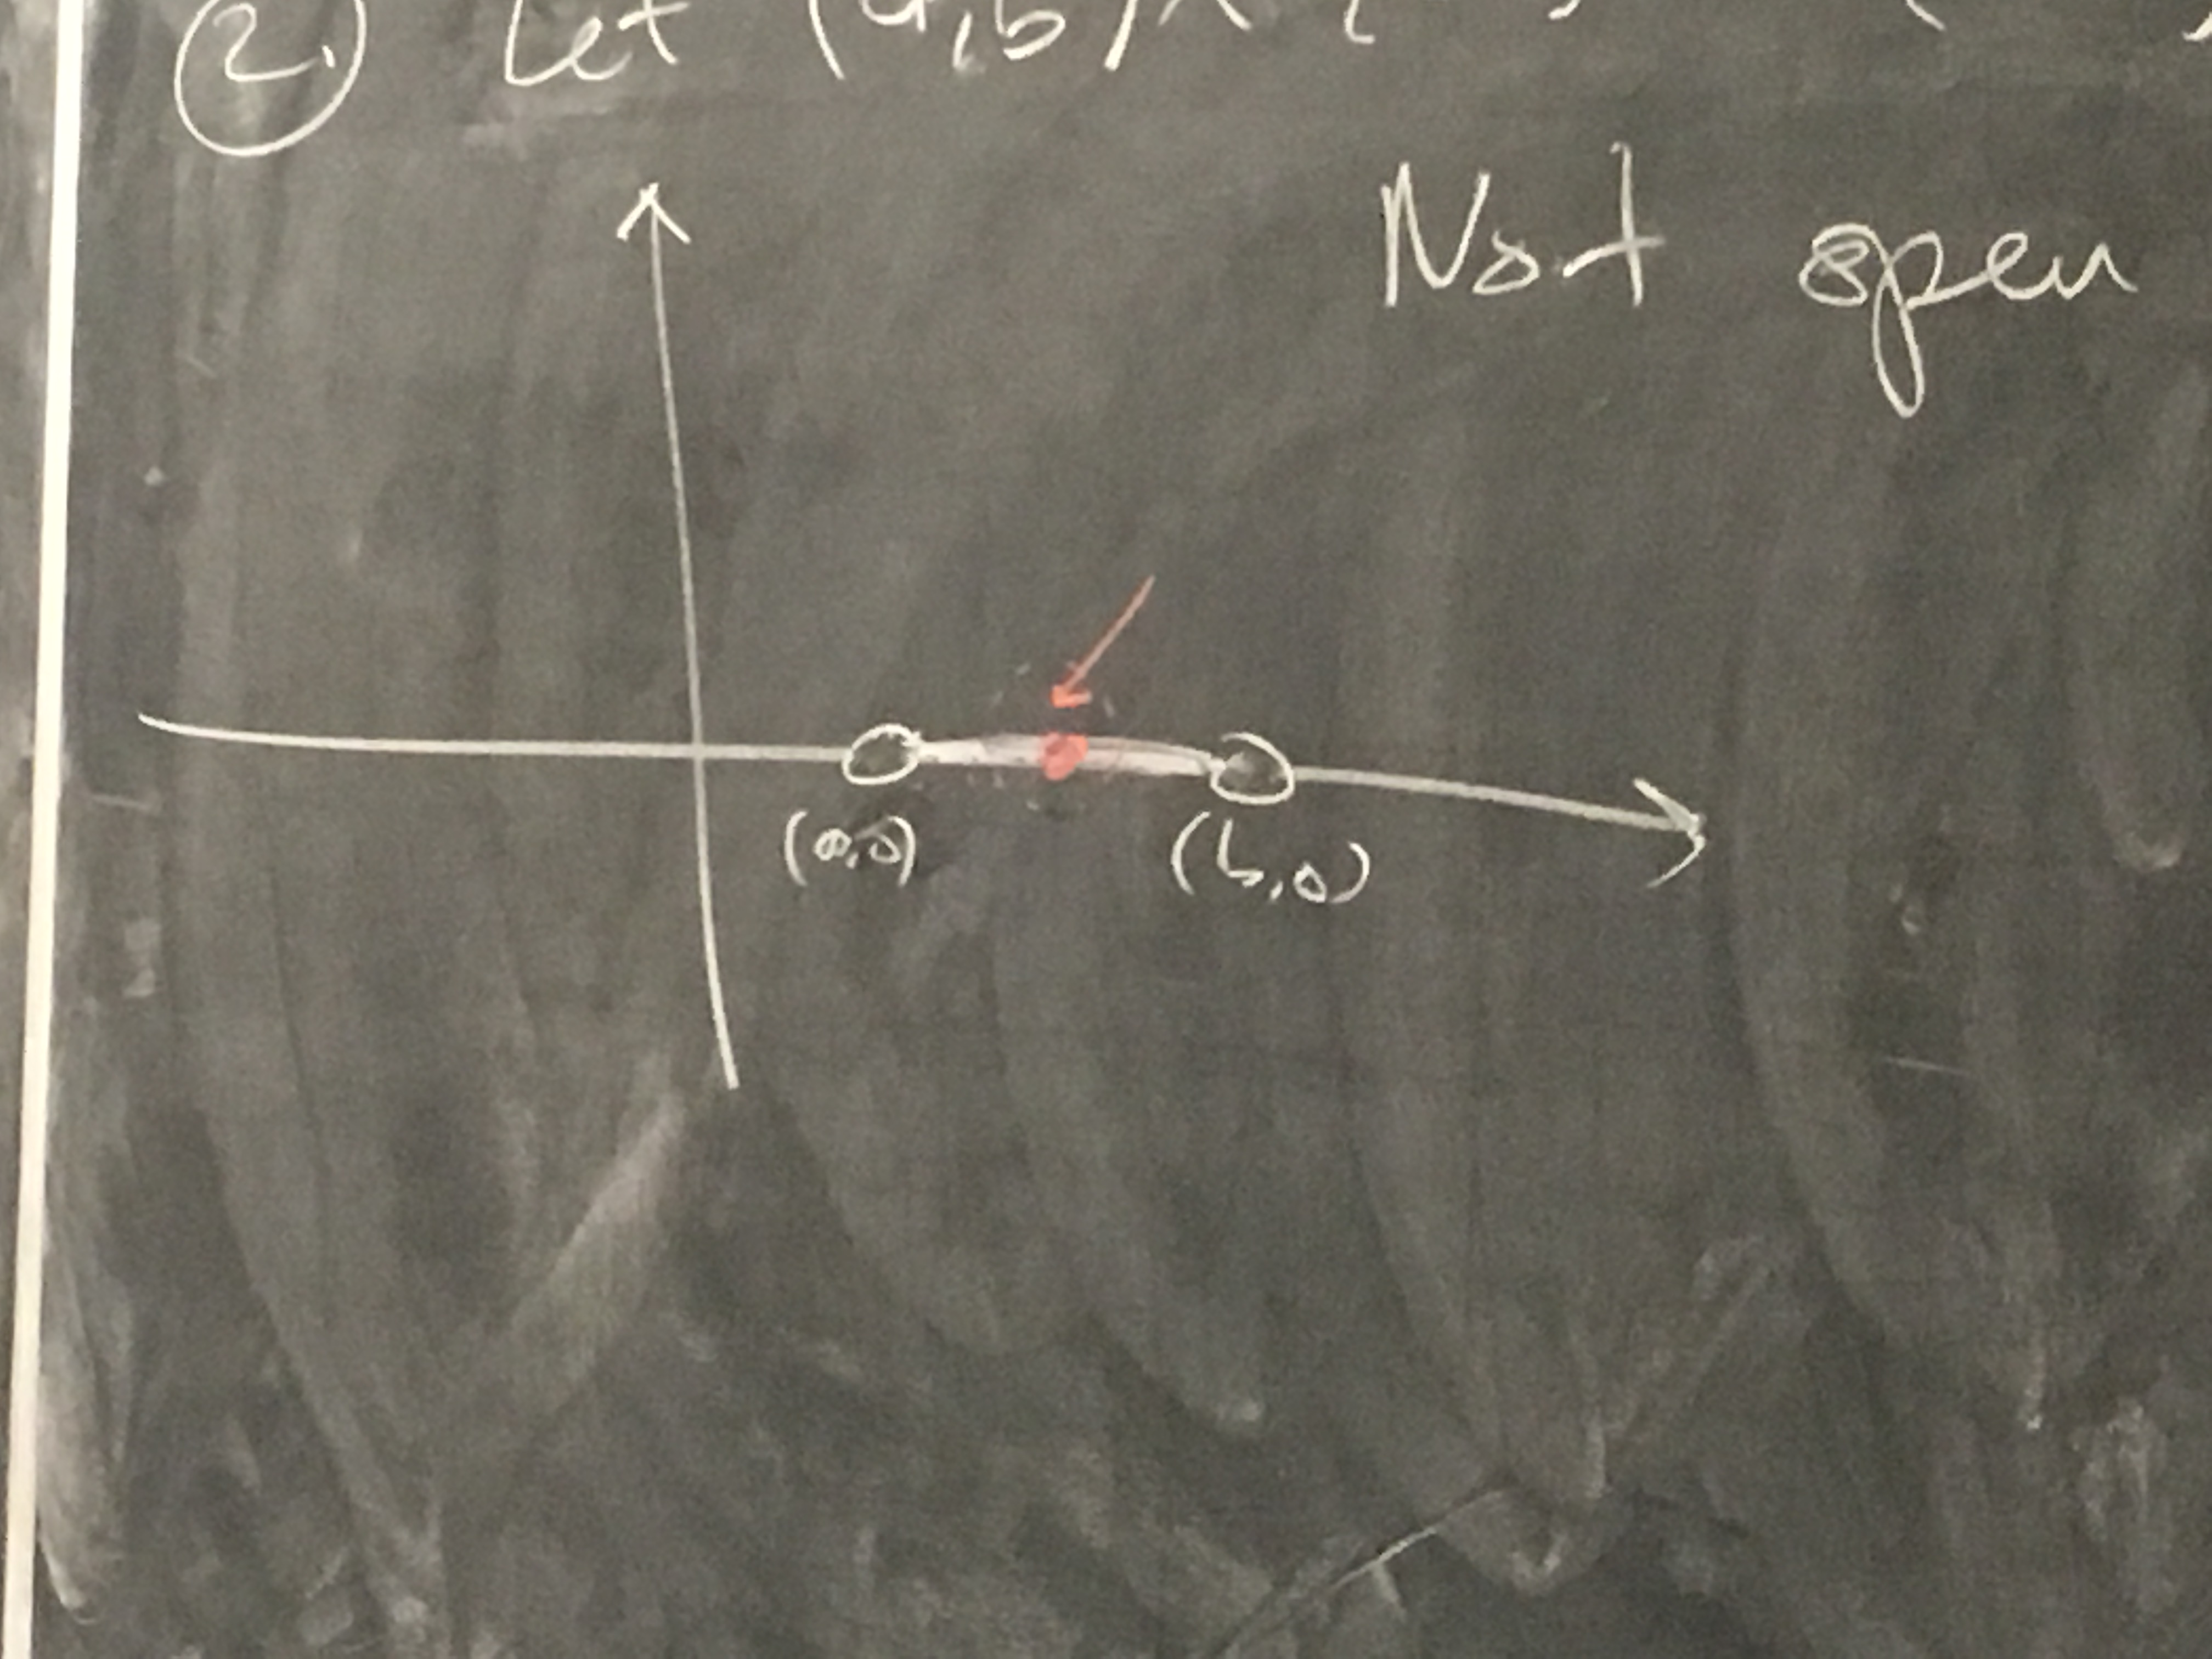
\includegraphics[scale=.05]{open_balls_2}
\end{center}

\item Consider $(a,b)\times(c,d)=\{(x,y):a<x<b, c<y<d\}$. (You might call this an open rectangle.) This set is open. 
\begin{center}
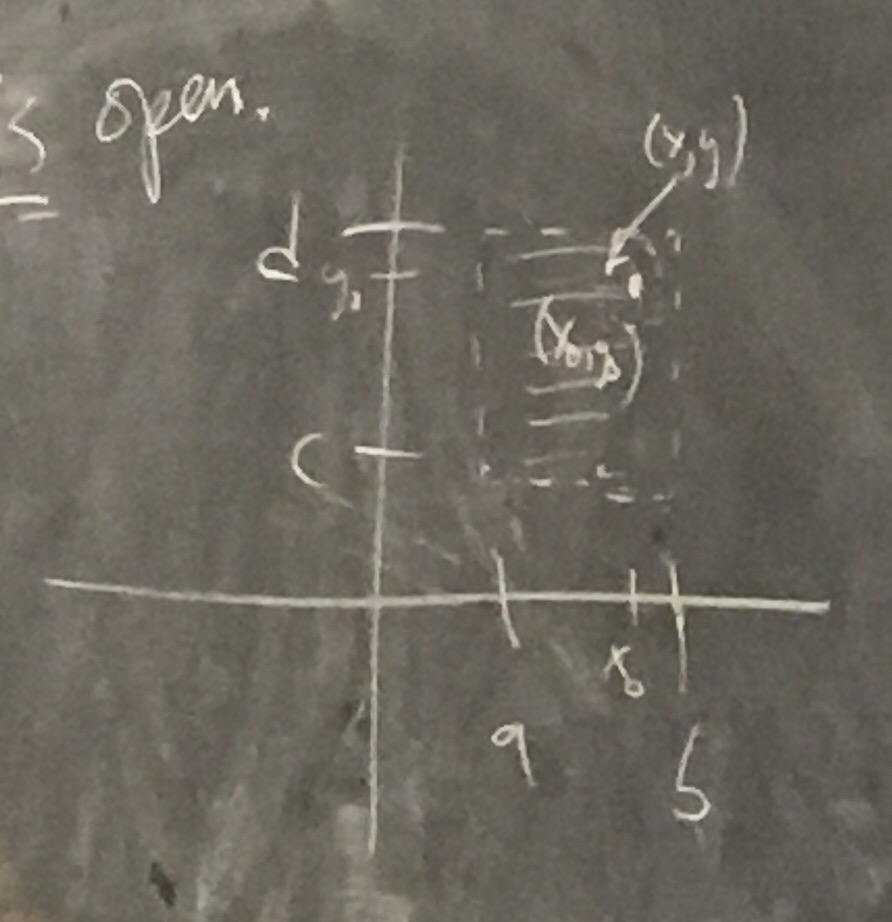
\includegraphics[scale=.2]{open_balls_3}
\end{center}

\item Consider $\{(x,y):y>x^2\}$. This set is open in $\R^2$.
Unsurprisingly, $\{(x,y):y\leq x^2\}$. This set is \emph{not} open in $\R^2$.
\begin{center}
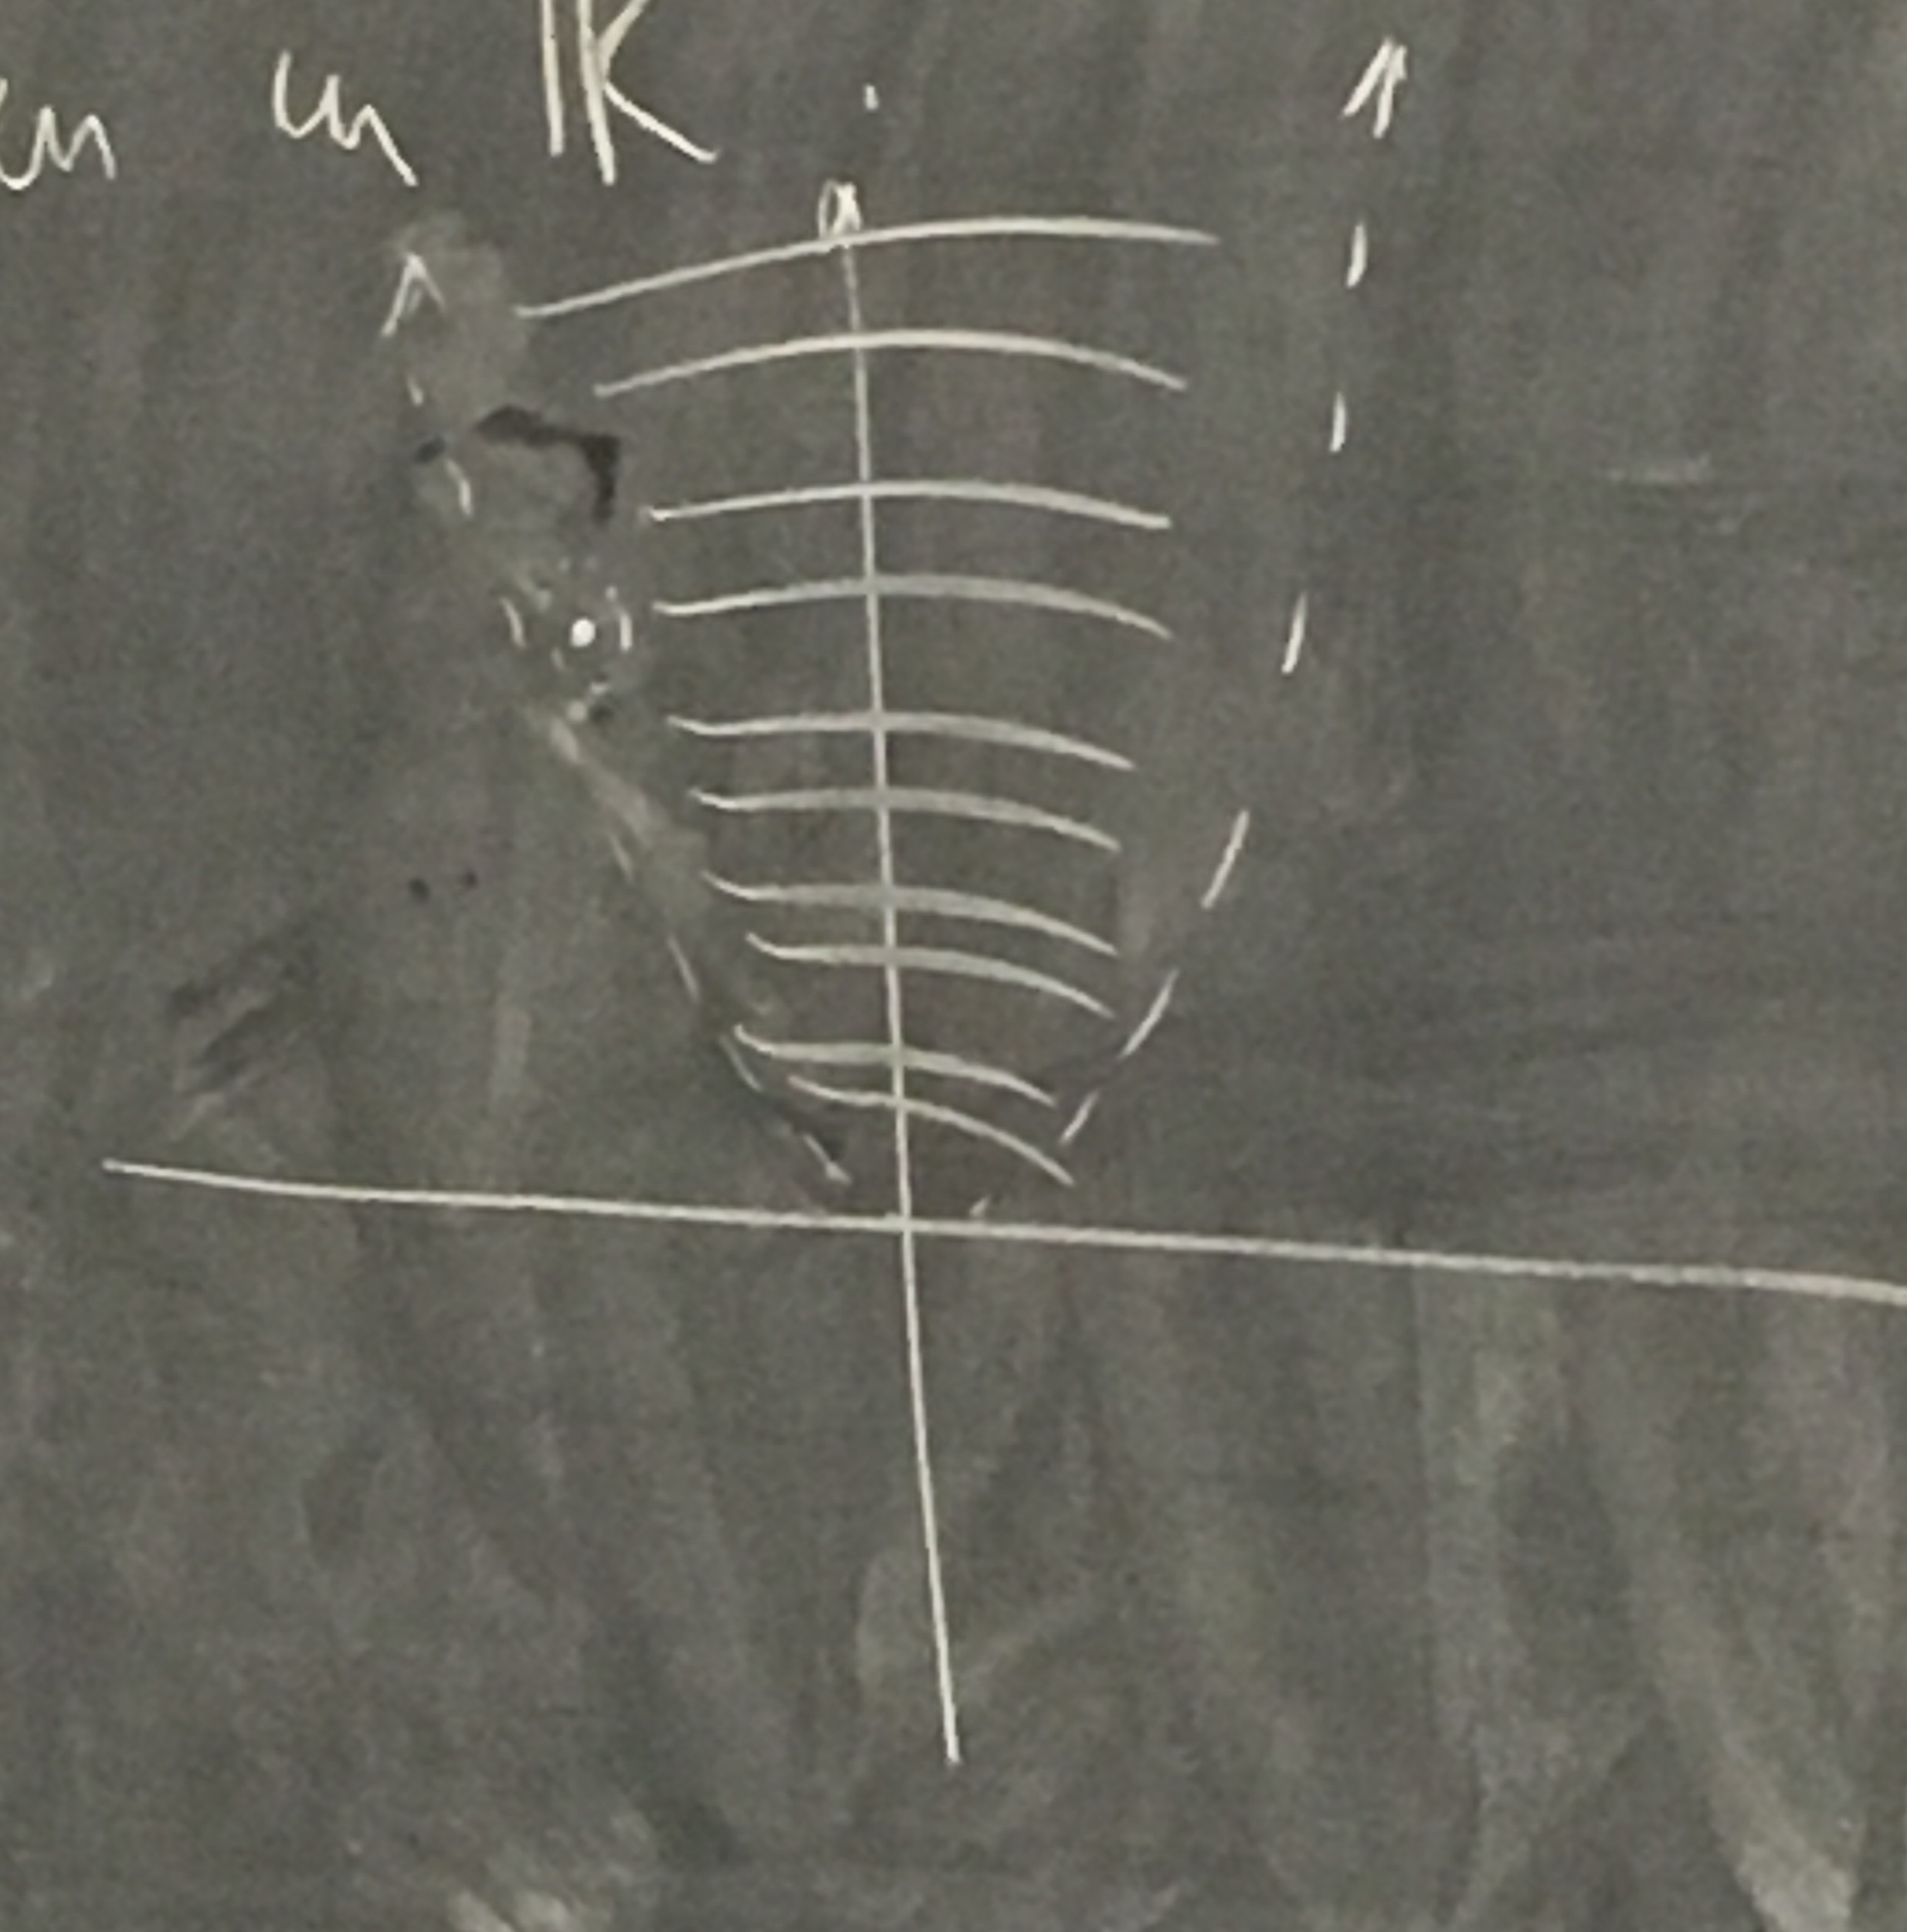
\includegraphics[scale=.07]{open_balls_4}
\end{center}

\item $\Q\subset\R$ is not open. You can't really graph this, but it's some kind of densely packed but not really continuous subset of the reals. So since any open ball will contain some points not in $\Q$, then $\Q$ is not open. 

\item Let $\vecb{x_0}\in \R^n$, with $R>0$.

Claim: $B(\vecb{x_0},R)$ is an open set. Now, we need to show that for any $\vecb{x}\in B(\vecb{x_0},R)$, there is an open ball containing $\vecb{x}$ which is a subset of $B(\vecb{x_0},R)$. To see this, let $\vecb{x}\in B(\vecb{x_0},R)$, and pick $r=R-\norm{\vecb{x}-\vecb{x_0}}$. 

\begin{center}
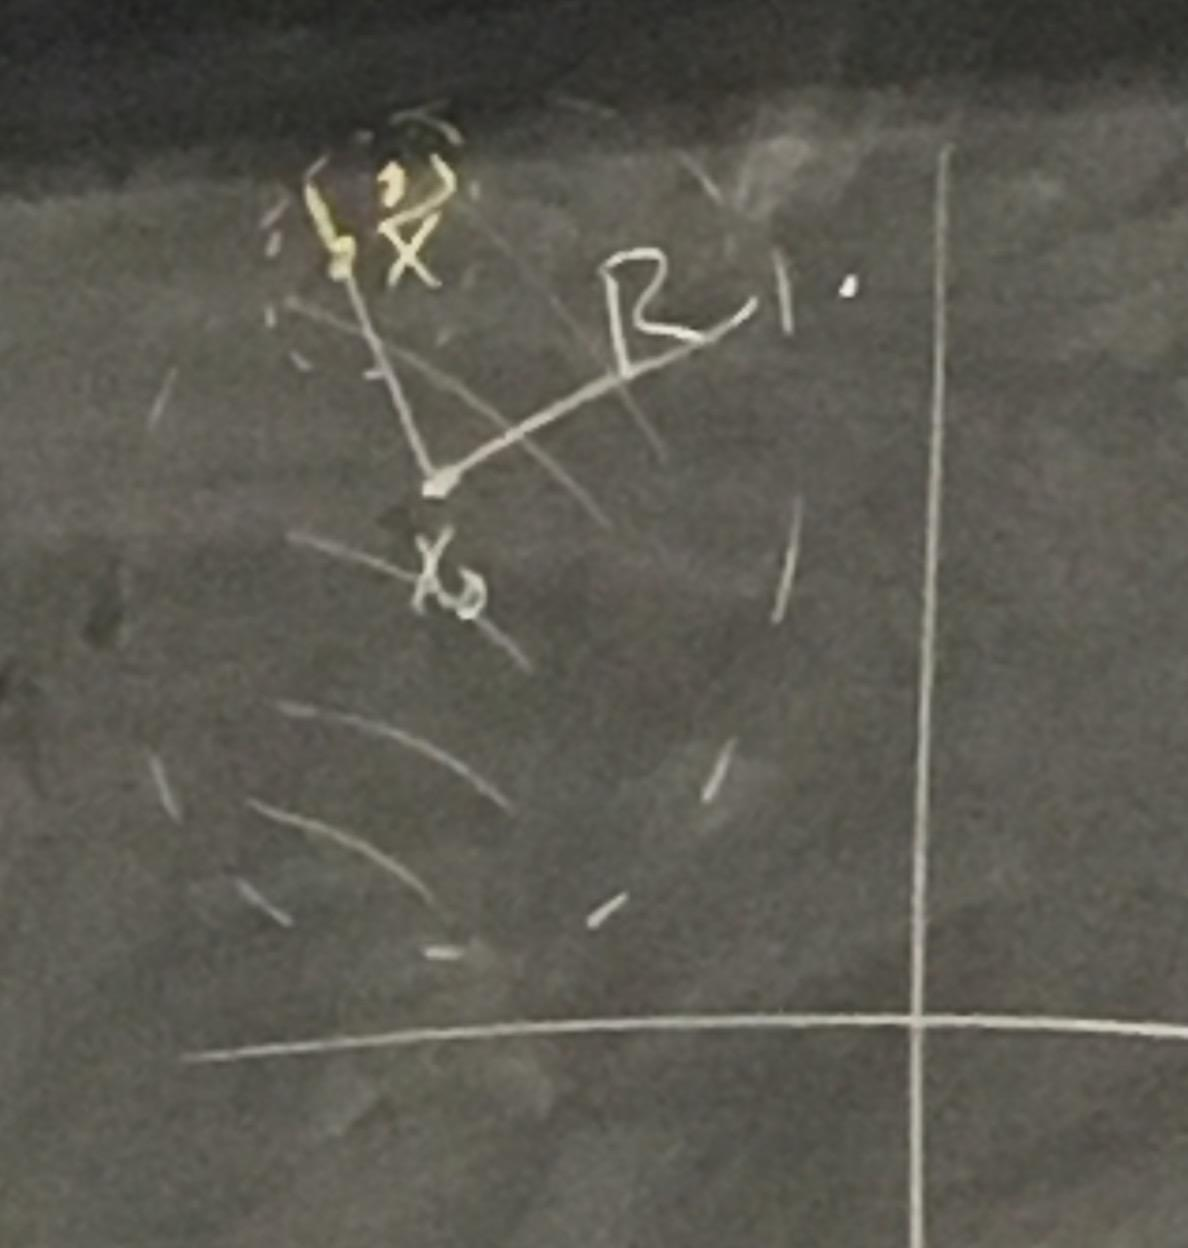
\includegraphics[scale=.12]{open_balls_5}
\end{center}

Now we check that $B(\vecb{x},r)\subseteq B(\vecb{x_0},R)$. Let 
(notes in image)

\end{enumerate}
\end{example*}

\begin{highlight}
\begin{proposition}[Characterization of open sets]\mbox{}
\begin{enumerate}[label=(\alph*)]
\item $\R^n$ is an open set. 
\item Let $\arbcoll{U}$ be a collection of open sets. Then $\arbcup{U}$ is open. 
\item Let $U_1, U_2$ be open sets. Then, $U_1\cap U_2$ is open. (by the way, this follows for any finite intersection). 
\item $\emptyset$ is open. 
\end{enumerate}
\end{proposition}
\end{highlight}

\begin{highlight}
\begin{definition*}
A set $C\subseteq R^n$ is \emph{closed} in $R^n$ iff $R^n-C$ is open. 
\end{definition*}
\end{highlight}

\begin{example*}\mbox{}
\begin{enumerate}
\item $\{\vecb{x_0}\}$ is closed in $R^n$ for any $\vecb{x_0}\in\R^n$. More generally, any finite collection of points $\{\vecb{x_1}, \vecb{x_2}, \ldots, \vecb{x_n}\}$ is closed in $R^n$. 

\item In $R^2$, $\{(x,y): x \text{ or } y \in \Z\}$ is closed. 
\begin{center}
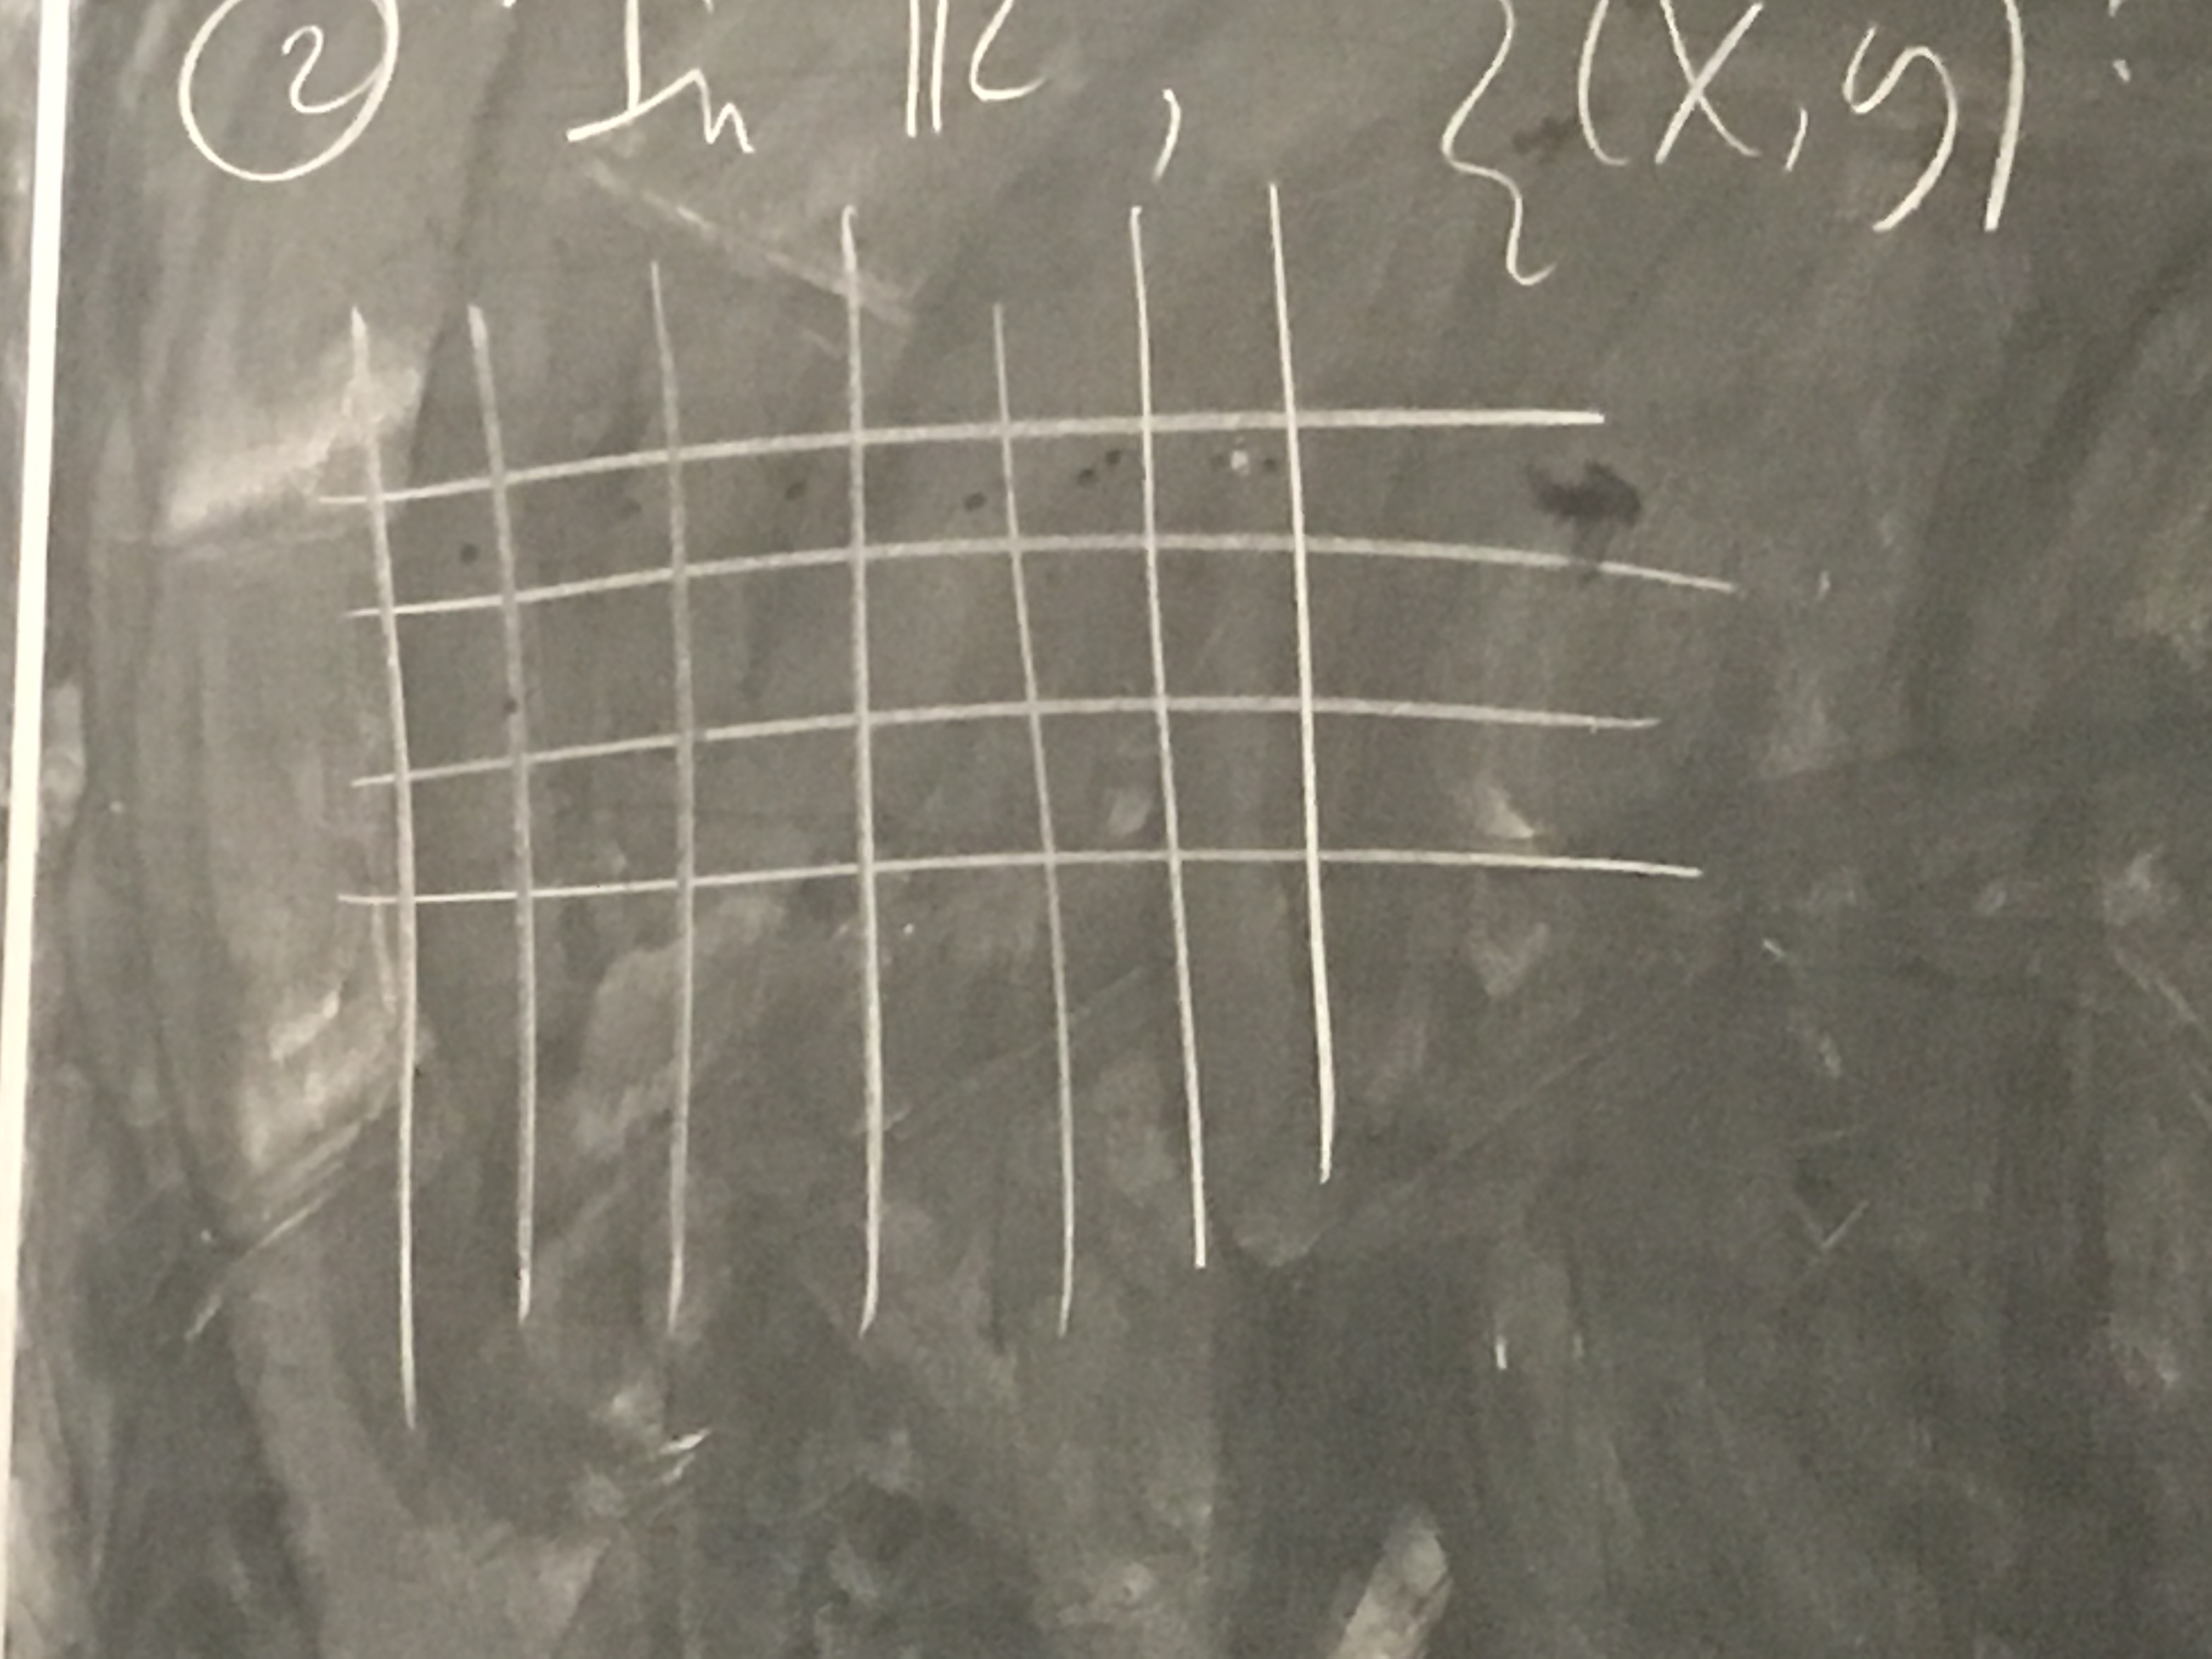
\includegraphics[scale=.04]{open_balls_6}
\end{center}

\item Consider the "closed ball" $\overline{B}(\vecb{x},r)=\{\vecb{x}:\norm{\vecb{x}-\vecb{x_0}}\leq r\}$. This set is closed. 
\begin{center}
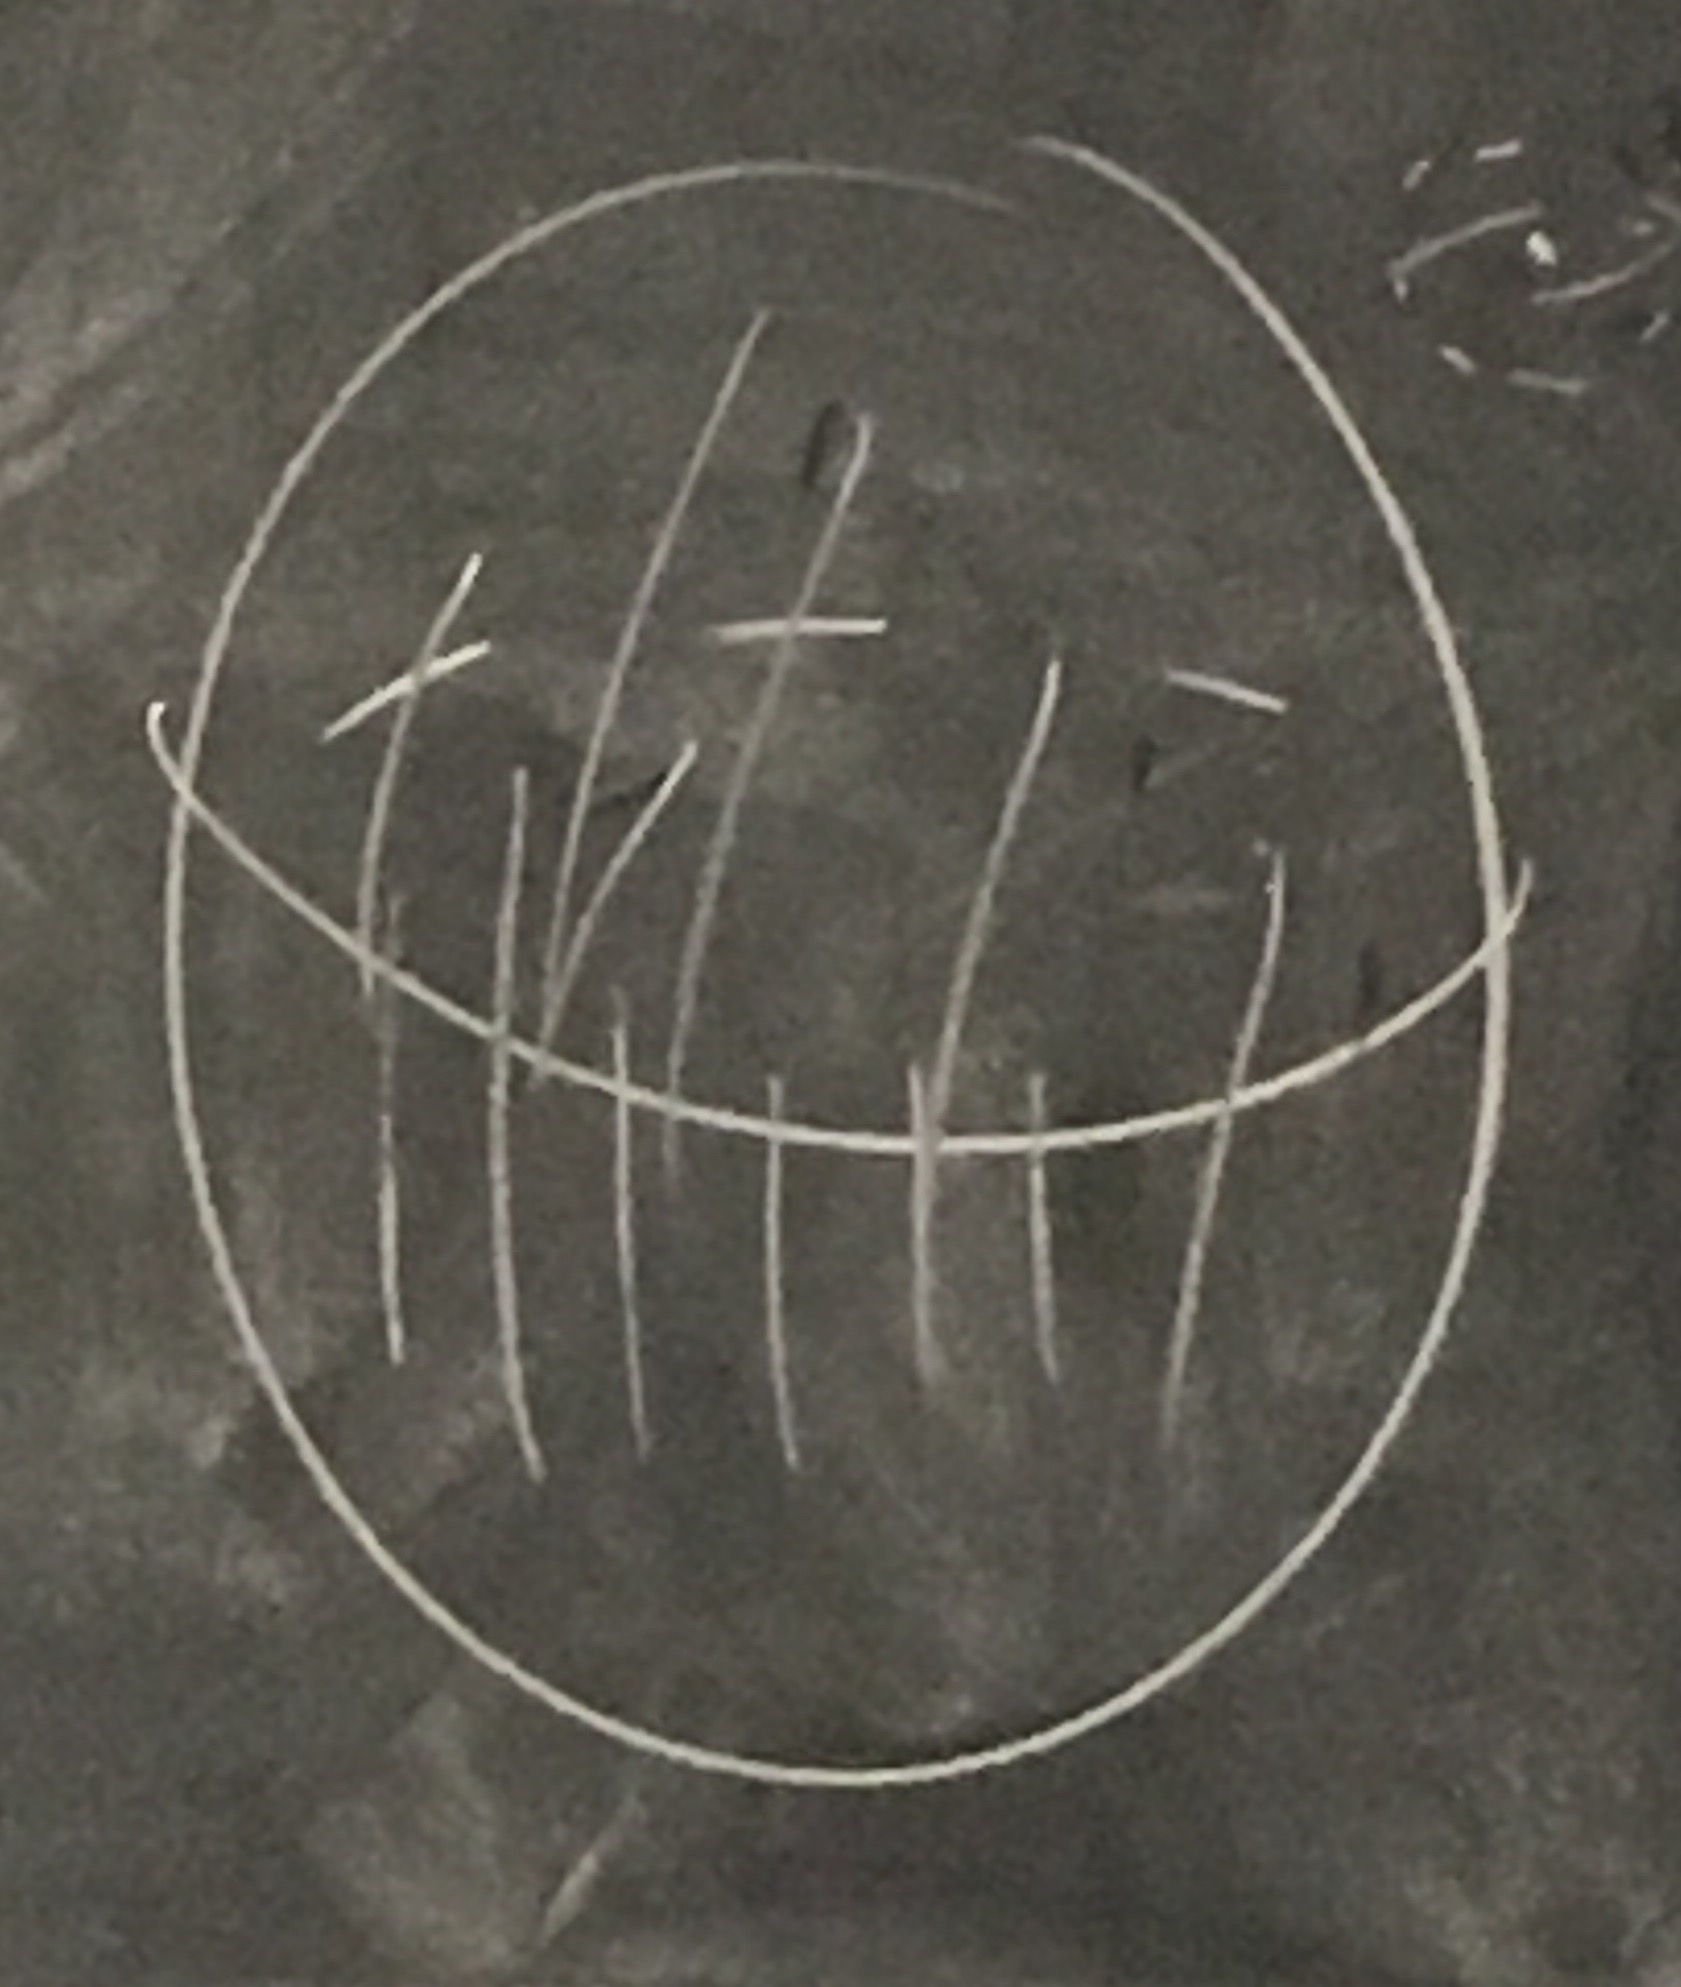
\includegraphics[scale=.07]{open_balls_7}
\end{center}

\item The set $\{(x,y):y=x^2\}$ is closed. 
\begin{center}
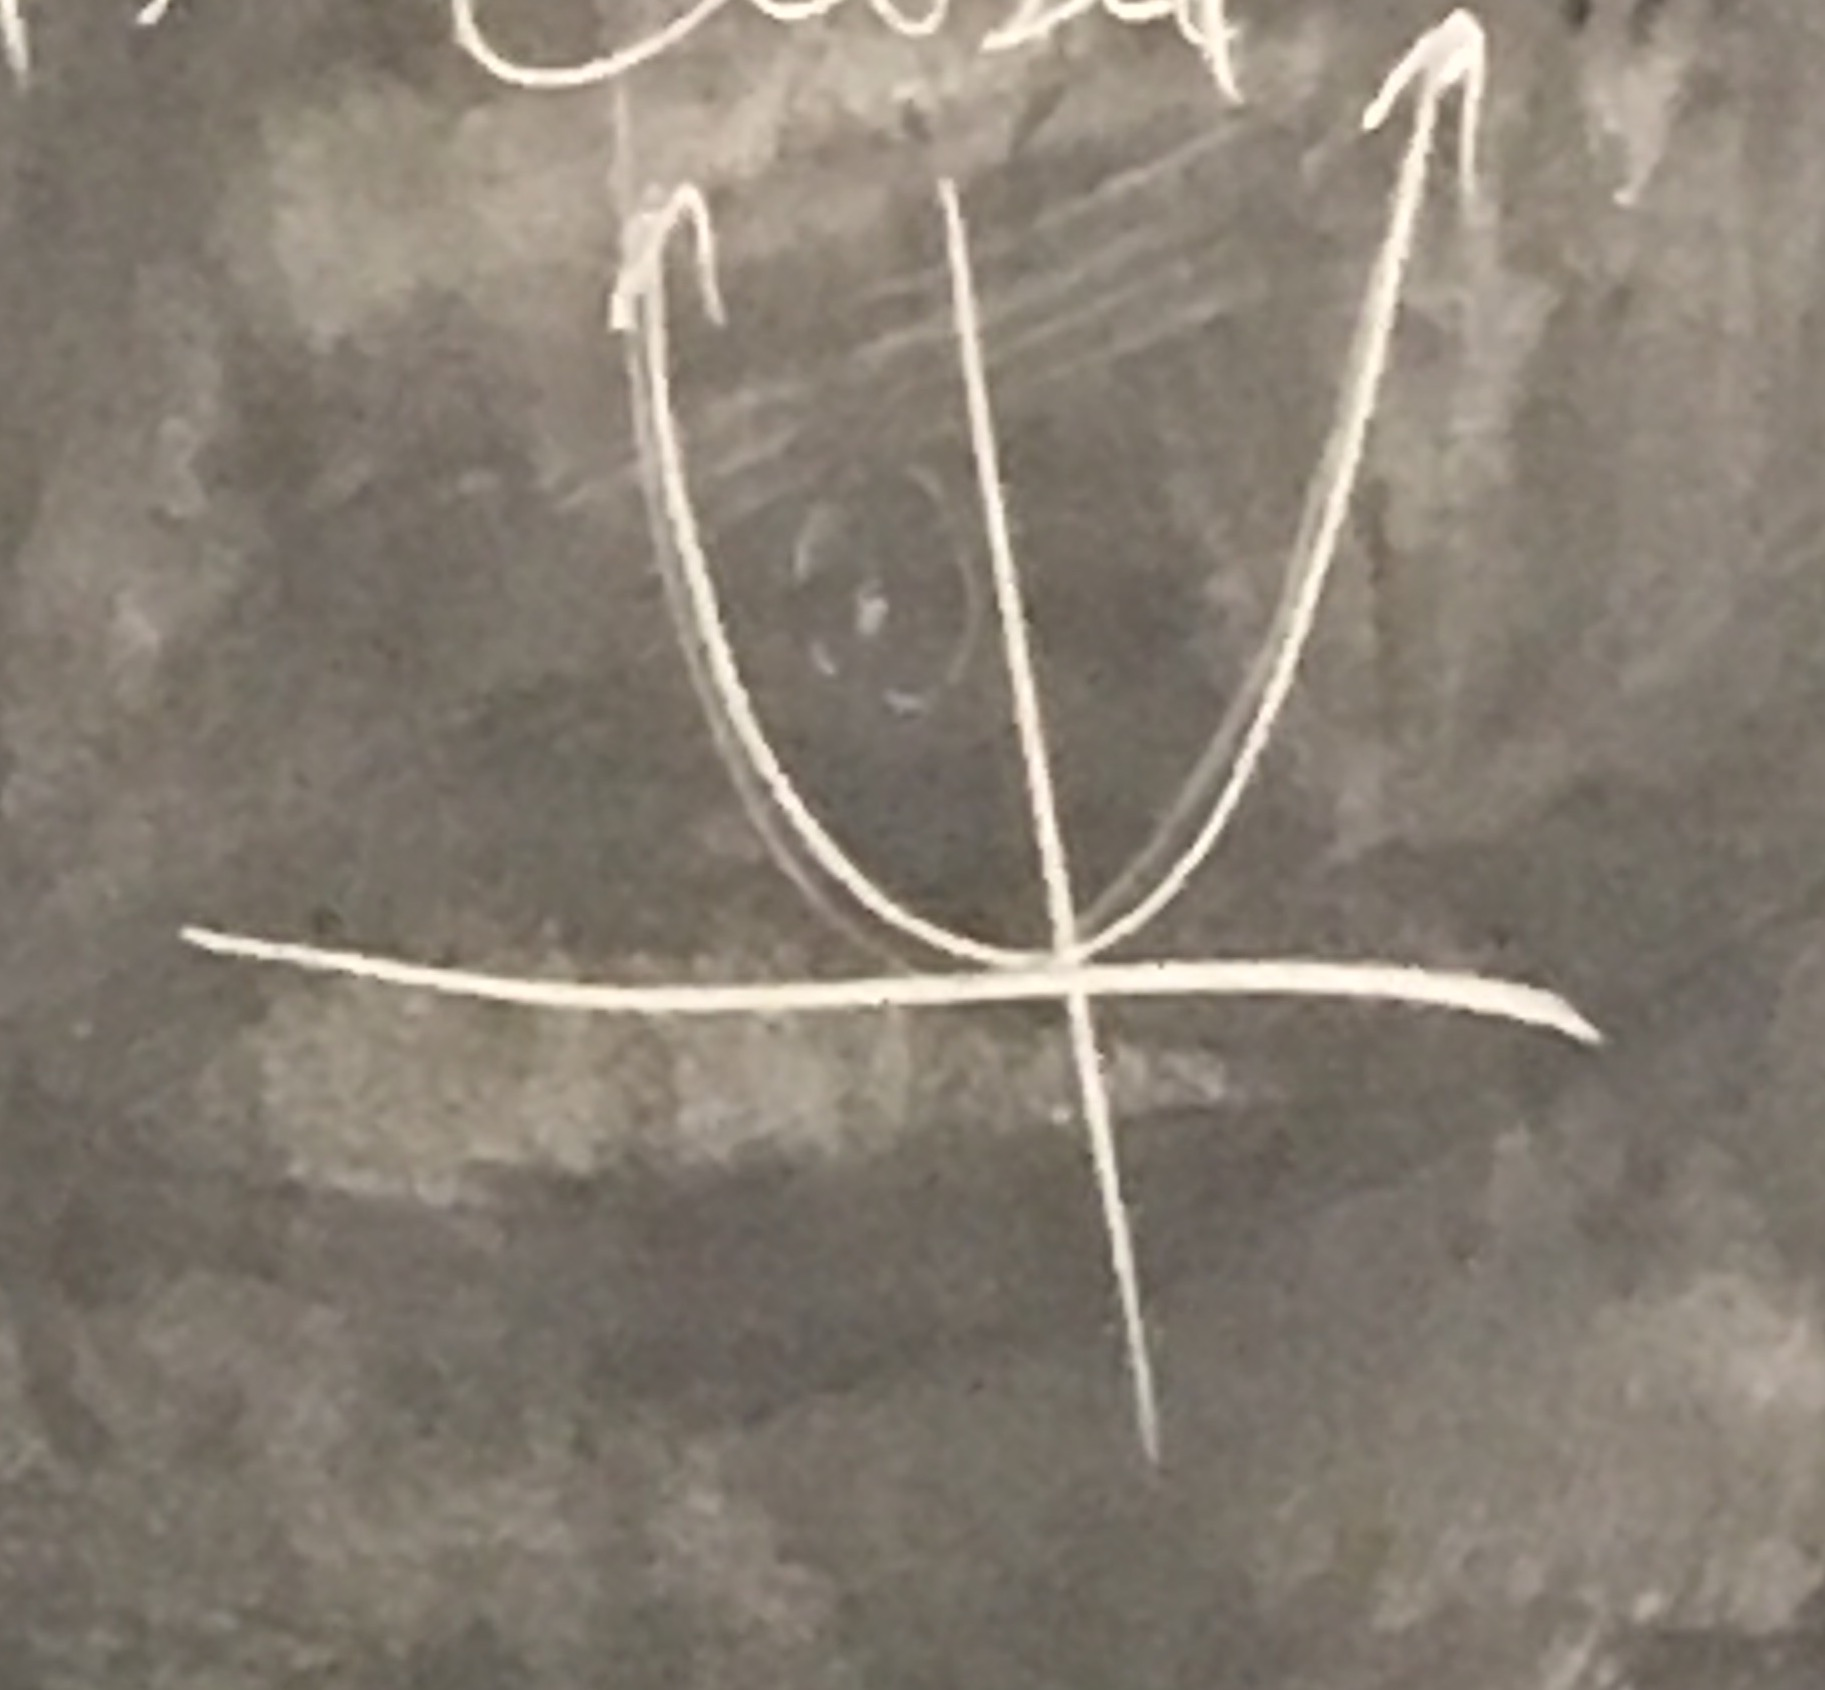
\includegraphics[scale=.07]{open_balls_8}
\end{center}

\end{enumerate}
\end{example*}

\begin{highlight}
\begin{definition*}
Let $S\subset\R^n$. Every point $\vecb{x}\in \R^n$ satisfies exactly one of the following statements:
\begin{enumerate}[label=(\alph*)]
\item There exists $r>0$ such that $B(\vecb{ x},r)\subset S$. 
\item There exists $r>0$ such that $B(\vecb{ x},r)\subset \R^n-S$. 
\item For every $r>0$, we have $B(\vecb{ x},r)\cap S\neq\emptyset$, and $B(\vecb{ x},r)\cap (\R^n-S)\neq\emptyset$.

We say that any point satisfying (a) is an element of the \emph{interior} of $S$, written int$(S)$. 

Any point satisfying (b) is an element of the \emph{exterior} of $S$, written ext$(S)$. 

Any point satisfying (c) is an element of the \emph{boundary} of $S$, written bdy$(S)$. 
\end{enumerate}
\end{definition*}
\end{highlight}

\begin{highlight}
\begin{remark*}
\begin{enumerate}
\item For any $S$, int$(S)\cup$ext$(S)\cup$bdy$(S)=\R^n$
\item int$(S)$ and wext$(S)$ are op[en sets. Also, $S$ is open if and only if int$(S)=S$. 
\end{enumerate}
\end{remark*}
\end{highlight}

\begin{example*}\mbox{}
\begin{enumerate}
\item $S=B(\vecb{x_0},r_0)$ in $R^n$. \\
int$(S)=S$\\
ext$(S)=\R^n-\closure{B}(\vecb{x_0},r_0)$
bdy$(S)=\{\vecb{y}:\norm{\vecb{x_0}-\vecb{y}}=r\}$
\item In $R^1$, Let $S=\Q$. \\
int$(\Q)=\emptyset$.\\
ext$(\Q)=\emptyset$.\\
bdy$(\Q)=\R$.\\
\end{enumerate}
\end{example*}

\subsection{Compactness}

\begin{highlight}
\begin{definition*}
Let $S\subset\R^n$. A collection of open sets $\script{U}=\arbcoll{U}$ is \emph{an open cover of $S$} if $S\subset \arbcup{U}$. 
\end{definition*}
\end{highlight}

\begin{highlight}
\begin{definition*}
$S\subset\R^n$ is \emph{compact} if every open cover has a finite subcover. 
\end{definition*}
\end{highlight}

This means: for every open cover $\arbcoll{U}$ of $S$, we can find $U_{\alpha_1}, U_{\alpha_2}, \ldots, U_{\alpha_n}$ in the collection with $S\subset U_{\alpha_1}\cup U_{\alpha_2}\cup \ldots\cup U_{\alpha_n}$.

\begin{example*}\mbox{}
\begin{enumerate}
\item In $R^1$, $S=\{0\}\cup\{\frac{1}{n}:n\in\N\}$ is compact.
\jpg{scale=.07}{compactness_1}
\begin{proof}
Let $\arbcoll{U}$ be an open cover of $S$. We have $0\in U_{\alpha_0}$ for some $\alpha_0\in\Gamma$. Since $U_{\alpha_0}$ is open, there is some $r>0$ such that $B(0,r)\subset U_{\alpha_0}$. We can then find $N$ such that $0<\frac{1}{n}<r$, so $\frac{1}{n}\in U_{\alpha_0}$ for all $n\geq N$. 

Now for each $1<m<N-1$, we can find $U_{\alpha_m}$ with $\frac{1}{m}\in U_{\alpha_m}$. Then $U_{\alpha_0}\cup U_{\alpha_1}\cup U_{\alpha_m}$ covers $S$. 
\end{proof}

\item In $\R^1$, $[0,\infty)$ in not compact. 
\jpg{scale=.08}{compactness_2}
\begin{proof}
$\{U_n\}_{n\in\N}$ given by $U_n=(-1,n)$ is an open cover, but no finite subcollection will cover $[0,\infty)$. 
\end{proof}

\item In $\R^1$, $\Q\cap[a,b]$ is not compact. 
\jpg{scale=.09}{compactness_3}
\begin{proof}
Select $\gamma_0$ irrational in $[a,b]$. Then the collection consisting of intervals $(a-1,\gamma_0-\frac{1}{n})$, $n\in\N$ together with $(\gamma_0, b+1)$ is an open cover with no finite subcover. 
\end{proof}
\end{enumerate}
\end{example*}

\begin{highlight}
\begin{theorem}
In $\R^1$, a closed interval $[a,b]$ is compact. 
\end{theorem}
\end{highlight}
\begin{proof}
Let $\arbcoll{U}$ be an open cover of $[a,b]$. Let 
$$A=\{x:a\leq x\leq b\text{, and }[a,x]\text{ is covered by finitely many sets from }\arbcoll{U}\}.$$
Goal: $b\in A$. If this is true, then we are done. \\
Note: $a\in A$, so $A\neq\emptyset$. \\
$A$ is bounded above by $b$, so $s=\sup(A)$ exists.\\
\textbf{Claim:} $s=b$. \\
\jpg{scale=.08}{compactness_thm_4_1}

If not, suppose $s<b$. Now, $s\in U_{\alpha_s}$ for some $\alpha_s\in\Gamma$. So we can find an open interval $(s-r, s+r)$ with $(s-r, s+r)\subset U_{\alpha_s}$. Select $r_2$ with $s-r<s<r_2<s+r$ and $r_2<b$. Furthermore, since $s=\sup(A)$, we can find $r_1\in A$ with $s-r<r_1<s<r_2\leq b<s+\epsilon$. Since $r_1\in A$, some finite subcollection of $\arbcoll{U}$ covers $[a,r_1]$. But then this subcollection, together with $U_{\alpha_s}$ covers $[a,r_2]$. Therefore, $r_2\in A$, contradicting the fact that $s=\sup(A)$ (since $r_2>s$). So, $\sup(S)=b$. \qedwhite
\mbox{}\\
\textbf{Claim:} $b\in A$. \\
\jpg{scale=.08}{compactness_thm_4_2}

Certainly $b\in U_{\alpha_b}$ for some $\alpha_b\in\Gamma$. So we can find some $r>0$ with $(b-r,b+r)\subset U_{\alpha_b}$. Since by the first claim, $b=\sup(A)$, there is $r_1\in A$ with $b-r<r_1\leq b$. Since $r_1\in A$, some finite subcollection of $\arbcoll{U}$ covers $[a,r_1]$. But this subcollection together with $U_{\alpha_b}$ covers $[a,b]$. So $b\in A$. 
\end{proof}

\begin{highlight}
\begin{proposition}
$U\subset \R^n$ is open if and only if for every $\vecb{x}\in U$, there is an open rectangle $\prod\limits_{i=1}^n(a_i,b_i)=(a,b)\times\ldots\times(a_n,b_n)$ with $\vecb{x}\in \prod\limits_{i=1}^n(a_i,b_i) \in U$. 
\end{proposition}
\end{highlight}
\begin{proof}($\implies$)
Suppose $U$ open and $\vecb{x}\in U$. We know there is some $r>0$ such that $\vecb{x} \in B(\vecb{x},r) \subset U$. Then 
$$\vecb{x}\in\left(x_1-\frac{r}{\sqrt{n}},x_1+\frac{r}{\sqrt{n}}\right)\times \ldots \left(x_n-\frac{r}{\sqrt{n}},x_n+\frac{r}{\sqrt{n}}\right)\subset B(\vecb{x},r)\subset U.$$

Now, to be rigorous, we should really justify this statement, but for the sake of time we will just say that you can use the Pythagorean theorem to verify.
\end{proof}
\begin{proof}($\impliedby$)
Suppose $U$ has the property that for all $\vecb{x}\in U$, there exists an open rectangle $\prod\limits_{i=1}^n(a_i,b_i)$ with $\vecb{x}\in\prod\limits_{i=1}^n(a_i,b_i)$. Let $r=\min_{i=1,\ldots, n}\{x_i-a_i, b_i-x_i\}$. Then $\vecb{x}\in B(\vecb{x},r)$. 

Now, we should technically show this rigorously, but $$\vecb{x}\in B(\vecb{x},r)\subset \prod\limits_{i=1}^n(a_i,b_i) \subset U,$$
So $U$ is open. We leave the proof of this detail as an unofficial exercise to the reader. 
\end{proof}

\noindent \textbf{Notation:} Given $\vecb{x}=(x_1, \ldots, x_n)\in \R^n$ and $\vecb{y}=(y_1, \ldots, y_m)\in \R^m$, we will sometimes write 
$$(\vecb{x},\vecb{y})=(x_1, \ldots, x_n, y_1, \ldots, y_m)\in \R^{n+m}.$$
Also, if $C\subset \R^n, D\subset \R^m,$ then we will sometimes write 
$$C\times D=\{(\vecb{x},\vecb{y}):\vecb{x}\in C, \vecb{y}\in D\}\subset \R^{n+m}.$$

\begin{highlight}
\begin{theorem}
Suppose $C\subset \R^n,  D\subset \R^m,$ are compact. Then $C\times D$ is compact in $\R^{n+m}$.
\end{theorem}
\end{highlight}
\begin{proof}
Let $\arbcoll{U}$ be an open cover of $C\times D$. Fix $\vecb{x}\in C$. For all $\vecb{y}\in D$, we can find some $U_{\alpha(y)}^x$ from the given open cover with $(\vecb{x},\vecb{y})\in U_{\alpha(y)}^x$. 

\jpg{scale=.06}{compactness_thm_6}

By Prop 5, there are open rectangles $V_{\alpha(y)}^x, W_{\alpha(y)}^x$ in $\R^n, \R^m$ respectively with 
$$(\vecb{x},\vecb{y})\in V_{\alpha(y)}^x\times W_{\alpha(y)}^x \subset U_{\alpha(y)}^x.$$
Notice $\{W_{\alpha(y)}^x\}_{y\in D}$ is an open cover of $D$. Since $D$ is compact, there exists a finite subcover $W_{\alpha({y_1})}^x, 
\ldots, W_{\alpha({y_{n_x}})}^x$. Also notice that $\vecb{x}\in \bigcap\limits_{j=1}^{n_x}V_{\alpha(y_j)}^x = V^x$ is open in $\R^n$. We now have that $V^x\times W_{\alpha({y_1})}^x, \ldots V^x\times W_{\alpha({y_{n_x}})}^x$ covers $\{x\}\times D$. \\

Now let $\vecb{x}$ vary. $\{V^x\}_{x\in C}$ is an open cover of $C$. So it has a finite subcover $V^{x_1}, \ldots, V^{x_M}$. We have $\bigcup_{i=1}^M\bigcup_{j=1}^{n_{x_i}} V_{\alpha(y_j)}^{x_i} \times W_{\alpha(y_j)}^{x_i}$ covers $C\times D$. So $\bigcup_{i=1}^M\bigcup_{j=1}^{n_{x_i}} U_{\alpha(y_j)}^{x_i}$ is a finite subcover of the original cover. 
\end{proof}

\begin{proposition*}[Corollary 6.1]
$[a,b]\times \ldots \times [a_n,b_n] \subset \R^n$ is compact. 
\end{proposition*}

\begin{highlight}
\begin{definition*}
$S\subset \R^n$ is \emph{bounded} if there exists some $M>0$ such that 
$$S\subset\closure{B}(\vecb{0},M).$$

(Equivalently, if $\norm{\vecb{x}} \leq M$ for all $\vecb{x}\in S$)
\end{definition*}
\end{highlight}

%theorem 7
\begin{highlight}
\begin{theorem}[Heine-Borel]
In $R^n$, $S$ is compact if and only if $S$ is closed and bounded. 
\end{theorem}
\end{highlight}
\begin{proof}($\implies$)
Suppose $C$ is compact. To see that $C$ is bounded, consider the open cover $\{B(\vecb{0},n):n\in \N\}$. Since $C$ is compact, is has a finite subcover, so there exists some $N\in \N$ such that $C\subset B(\vecb{0},N)$.

To see that $C$ is closed, let $\vecb{x_0}\in \R^n-C$. 
\jpg{scale=.06}{compactness_thm_8_1}
For every $\vecb{y}\in C$, there is $r_y>0$ such that $B(\vecb{y},r_y)\cap B(\vecb{x},r_y)=\emptyset$. Now $\{B(\vecb{y}, r_y)\}_{y\in C}$ is an open cover of $C$, so it has a finite subcover $B(\vecb{y_1}, r_{y_1}), \ldots, B(\vecb{y_m}, r_{y_m})$. Let $V=\bigcap_{i=1}^m B(\vecb{x_0}, r_{y_i})$ is an open set containing $x_0$ such that $C\cap V=\emptyset$, so $C$ is closed. 
\end{proof}
\begin{proof}($\impliedby$)
Suppose $C$ is closed and bounded. 
\jpg{scale=.06}{compactness_thm_8_2}
Let $\arbcoll{U}$ be an open cover of $C$. Since $C$ is bounded, $C\subset \prod\limits_{i=1}^n[a_i, b_i]$ which is compact by an earlier theorem. Observe that $\arbcoll{U}\cup (\R^n-C)$ is an open cover of $\prod\limits_{i=1}^n[a_i, b_i]$. Since $\prod\limits_{i=1}^n[a_i, b_i]$ is compact, it has a finite subcover $U_{\alpha_1}, \ldots, U_{\alpha_n}, \R^n-C$. Which also must cover $C$, and we are done since $U_{\alpha_1}, \ldots, U_{\alpha_n}$ is a finite subcollection of $\arbcoll{U}$. 
\end{proof}

\begin{example*}\mbox{}
\begin{enumerate}
\item $\{0\}\cup\{\frac{1}{n}:n\in N\}$ is closed and bounded. 

\item $[0,\infty)$ is closed, but not bounded. 

\item $\Q\cap [a,b]$ is bounded, but not closed. 
\end{enumerate}
\end{example*}

\pagebreak
\section{Continuity}

%\jpg{scale=.1}{Discontinuous_700}

\begin{highlight}
\begin{definition*}[$\delta-\epsilon$ definition of continuity]\mbox{}\\
We say that $f:A\subset \R^n \to \R^m$ is \emph{continuous at $\vecb{a}\in A$} if, for any $\epsilon >0$, there is $\delta>0$ such that 
\begin{itemize}
\item If $\vecb{x}\in A$ and $\norm{\vecb{x}-\vecb{a}}<\delta$, then $\norm{f(\vecb{x})-f(\vecb{a})}<\epsilon$. 
\item If $\vecb{x}\in B(\vecb{a},\delta)$, then $f(\vecb{x})\in B(f(\vecb{a}),\epsilon)$. 
\end{itemize}
The two phrasings above are equivalent. 
\end{definition*}
\end{highlight}

\begin{highlight}
\begin{definition*}
We will say that $f:A\subset \R^n \to \R^m$ is \emph{continuous} (or \emph{continuous on $A$}) if it is continuous at all $\vecb{a}\in A$. 
\end{definition*}
\end{highlight}

\begin{highlight}
\begin{definition*}
Given $f:A\subset \R^n \to \R^m$, we can write it as 
$$f(x_1, \ldots, x_n)=(f_1(x_1, \ldots, x_n), f_2(x_1, \ldots, x_n), \ldots, f_m(x_1, \ldots, x_n),$$
Where $f_i:A\to \R$. We refer to $f_i$ as the \emph{$i$th component function} of $f$. 
\end{definition*}
\end{highlight}

\begin{highlight}
\begin{proposition}
Let $f:A\subset \R^n \to \R^m$ be a function. $f:A\to\R^m$ is continuous if and only if each $f_i:A\to \R$ is continuous. 
\end{proposition}
\end{highlight}
\begin{proof}$(\implies)$
Assume $f$ is continuous. Given $\epsilon>0$, and any $\vecb{a}\in A$, pick $\delta$ so that 
$$\norm{\vecb{x}-\vecb{a}}<\delta \text{ implies } \norm{f(\vecb{x})-f(\vecb{a})}<\epsilon.$$
But for  $\norm{\vecb{x}-\vecb{a}}<\delta$, 
$$\abs{f_i(\vecb{x})-f_i(\vecb{a})}\leq \norm{f(\vecb{x})-f(\vecb{a})}<\epsilon.$$
So each $f_i$ is continuous at $\vecb{a}$ for any $\vecb{a}\in A$. 
\end{proof}
\begin{proof}$(\impliedby)$
Conversely, suppose that each $f_i:A\to \R$ is continuous at $\vecb{a}$. Let $\epsilon>0$. For each $i$, we can find $\delta_i>0$ such that 
$$\vecb{x}\in A, \norm{\vecb{x}-\vecb{a}}<\delta \text{ implies } \norm{f_i(\vecb{x})-f_i(\vecb{a})}<\frac{\epsilon}{\sqrt{m}}.$$
Let $\delta=\min_{i\in \{1, \ldots m\}}(\delta_i)$. Then if $\vecb{x}\in A$, $\norm{\vecb{x}-\vecb{a}}<\delta$, 
$$\text{(gnarly equations, see picture)}$$
and we are done. 
\end{proof}

\begin{highlight}
\begin{proposition}\mbox{}
\begin{enumerate}[label=(\roman*)]
\item If $f,g:A\subset \R^n \to \R^m$ are continuous, then $f+g:A \to \R^m$ is continuous.
\item If $f,g:A\subset \R^n \to \R$ are continuous, then $fg:A \to \R$ is continuous and $\frac{f}{g}:A-\{\vecb{x}:g(\vecb{x})=0\} \to \R$ is continuous.
\item If $f,g:A\subset \R^n \to \R^m$ are continuous, then $\inner{f}{g}:A \to \R$ is continuous.
\end{enumerate}
\end{proposition}
\end{highlight}
\begin{proof}(iii)\\
\textbf{scratch work for the proof:} 
Note: vector symbols are omitted here for brevity.
\[\begin{array}{rcl}
&&\abs{\inner{f(x)}{g(x)}}-\inner{f(a)}{g(a)}\\
&=&\abs{\inner{f(x)}{g(x)-g(a)}-\inner{f(a)-f(x)}{g(a)}}\\
&=&\abs{\inner{f(x)}{g(x)-g(a)}+\inner{f(x)-f(a)}{g(a)}}\\
&\leq&\abs{\inner{f(x)}{g(x)-g(a)}}+\abs{\inner{f(x)-f(a)}{g(a)}}\\%triangle inequality
&\leq&\norm{f(x)}\norm{g(x)-g(a)}+\norm{f(x)-f(a)}\norm{g(a)}\\% cauchy schwarz
&\leq&(\norm{f(a)}+1)\norm{g(x)-g(a)}+\norm{f(x)-f(a)}\norm{g(a)}\\
&\leq& \frac{\epsilon}{2} + \frac{\epsilon}{2} = \epsilon
\end{array}\]

(check picture for the actual proof)
\end{proof}

\begin{example*}
Let $f:\R^2:\R$ be defined by 
\[f(x,y)=
\begin{cases}
\frac{x^2}{x^2+y^2} & (x,y)\neq(0,0)\\
0 & (x,y)=(0,0)\\
\end{cases}_.\]
If $(x_0,y_0)\neq(0,0)$, $f$ is continuous at $(x_0,y_0)$ because it is a sum and quotient of continuous functions with nonzero denominator. However, $f$ is not continuous at $(0,0)$. Observe that for all $x=0$, $f(x,y)=0$, but for all $y=0$, $x\neq0$, $f(x,y)=1$. Let $\epsilon=\frac{1}{2}$. Then for any $\delta>0$, $\norm{(\frac{\delta}{2},0)-(0,0)}<\delta$, but $\abs{f(\frac{\delta}{2},0)-f(0,0)}=1>\epsilon$. 
\end{example*}

%10
\begin{highlight}
\begin{theorem}
Any linear transformation $T:\R^n\to\R^m$ is continuous. 
\end{theorem}
\end{highlight}
\begin{proof}
We can write 
$$T(x_1, \ldots , x_n)=\left(\sum_{k=1}^n a_{1k} x_k, \sum_{k=1}^n a_{2k} x_k, \ldots, \sum_{k=1}^n a_{mk} x_k\right),$$
for some real numbers $a_{ij}, 1\leq i\leq m, 1\leq j \leq n$. Notice $T_i(\vecb{x})=\inner{\vecb{x}}{\vecb{a_i}}$ where $\vecb{a_i}=\langle a_{i1}, \ldots, a_{in}\rangle$. So each $T_i$ is continuous by Prop 9, and so $T$ is continuous by Prop 8.
\end{proof}

\begin{definition*}
For $f:\R^n\to\R^m$, and $U\subset \R^m$, we write $\preimage{f}{U}$ to mean the \emph{preimage} of $U$ in $f$, that is, 
$$\preimage{f}{U}=\{x:f(x)\in U\}$$
so, $\preimage{f}{U}\subset \R^n$. 
\end{definition*}

\begin{highlight}
\begin{theorem}
Let $f:(A\subset\R^n)\to\R^m$ be continuous. The following are equivalent:
\begin{enumerate}
\item $f$ is continuous.
\item For every open set $U\subset \R^m$, we have $\preimage{f}{U}=(A\cap V)$, where $V$ is open in $\R^n$. 
\item For every closed set $C\subset \R^m$, we have $\preimage{f}{C}=(A\cap D)$, where $D$ is closed in $\R^n$.
\end{enumerate}
\end{theorem}
\end{highlight}
The following proofs assume $f$ is defined on all of $\R^n$, for simplicity. 
\begin{proof}(1)$\implies$(2)\\
Let $U$ be an open set in $\R^m$, and $\vecb{a}\in \preimage{f}{U}$. Note that $f(\vecb{a})\in U$, and since $U$ is open there exists $\epsilon>0$ such that $B(f(\vecb{a}),\epsilon)\subset U$. Since $f$ is assumed continuous, there exists $\delta>0$ such that $\vecb{x}\in B(\vecb{a},\delta)$ implies $f(\vecb{x})\in B(f(\vecb{a}), \epsilon)\subset U$. This implies $\vecb{x}\in \preimage{f}{U}$. We have $b(\vecb{a}, \delta)\subset \preimage{f}{U}$, showing $\preimage{f}{U}$ is open. 
\end{proof}
\begin{proof}(2)$\implies$(1)\\
Assume (2). Let $\epsilon>0$, $\vecb{a}\in \R^n$. We know $B(f(\vecb{a}),\epsilon)$ is open in $\R^m$, so by assumption	$\preimage{f}{B(f(\vecb{a}),\epsilon)}$ is open in $\R^n$, and $\vecb{a}\in \preimage{f}{B(f(\vecb{a}),\epsilon)}$. So there exists $\delta>0$ such that $B(\vecb{a},\delta)\subset \preimage{f}{B(f(\vecb{a}),\epsilon)}$. In other words, $\vecb{x}\in B(\vecb{a}, \delta)$ implies $f(\vecb{x})\in B(f(\vecb{a}),\epsilon)$. So $f$ is continuous. 
\end{proof}
\begin{proof}(2)$\iff$(3)\\
$$\R^n-\preimage{f}{S}=\preimage{f}{\R^m-S} \text{ for any } S\in \R^m.$$
\end{proof}

\begin{highlight}
\begin{corollary}
Suppose $f:A\subset \R^n\to\R^m$ is continuous, and $g:B\subset \R^m\to R^\ell$ is continuous, with $f(A)\subset B$. \\
Then, $g\circ f:A\subset \R^n\to\R^\ell$ is continuous. 
\end{corollary}
\end{highlight}

\pagebreak
\begin{theorem}
Let $f:(C\subset\R^n)\to\R^m$ be continuous, with $C$ compact. Then, $f(C)$ is bounded.
\end{theorem}
\begin{proof}
Observe that $\{\preimage{f}{B(\vec{0},n):n\in \N}\}$ is an open cover for $C$. So it has a finite subcover. Thus, there is some $N$ such that $C\subset \preimage{f}{B(\vec{0},N)}$, so $f(C)\subset B(\vec{0},N)$. 
\end{proof}

\begin{highlight}
\begin{theorem}
Let $f:(C\subset\R^n)\to\R^m$ be continuous, with $C$ compact. Then, $f(C)$ is compact.
\end{theorem}
\end{highlight}
\begin{proof}
Let $\arbcoll{U}$ be an open cover of $f(C)$. Then, $\{\preimage{f}{U_\alpha}\}_{\alpha\in \Gamma}$ is an open cover of $C$. So, there is a finite subcover $\{\preimage{f}{U_{\alpha_i}}\}_{i=1}^{n}$. Then, $\{{U_{\alpha_i}}\}_{i=1}^{n}$ covers $C$. 
\end{proof}

\begin{highlight}
\begin{theorem}[Extreme Value Theorem]
Let $f:(C\subset\R^n)\to\R$ be continuous, with $C$ compact. Then, there exist $\vecb{x}_0$, $\vecb{x}_1 \in C$ with $f(\vecb{x}_0)\leq f(\vecb{x})\leq f(\vecb{x}_1)$ for all $\vecb{x}\in C$. 
\end{theorem}
\end{highlight}
\begin{proposition*}
We know $f(C)$ is bounded above, so $\alpha=\sup f(C)$ exists. Suppose $\alpha\not\in C$.  Then $g:C\to \R^m$ 
$$g(\vecb{x})=\frac{1}{\alpha-f(\vecb{x})}$$
is a continuous function. So $g$ is bounded on $C$, so there is $M$ such that 
$$\frac{1}{\alpha-f(\vecb{x})}=g(\vecb{x})\leq M$$
for all $\vecb{x}\in C$. Equivalently, 
$$f(\vecb{x})\leq \alpha-\frac{1}{M}$$ 
for all $\vecb{x}\in C$, which contradicts $\alpha=\sup f(C)$. 
\end{proposition*}

\subsection{Some reminders about Linear Transformations}

Recall from your Linear Algebra class that by definition, a linear transformation $T:\R^n\to R^m$ has the following properties:
\begin{itemize}
\item $T(\vecb{x}_1+\vecb{x}_2)=T(\vecb{x}_1)+T(\vecb{x}_2)$
\item $T(\alpha\vecb{x})=\alpha T(\vecb{x})$
\end{itemize}

So, as a consequence of this, $T(\vec{0})=\vec{0})$. Also, let $\vecb{e}_1, \ldots \vecb{e}_n$ be the standard basis, that is, 
$$\vecb{e}_j=(0,\ldots, 1, \ldots, 0),$$
with the 1 in the $j$th coordinate. Another fact we know is that any linear transformation $T$ is completely determined by $T(\vecb{e}_1), \ldots, T(\vecb{e}_n)$, since any vector is some linear combination of basis vectors. 

\section{Derivatives}

\subsection{Vector-valued multi-variable functions}

\begin{highlight}
\begin{definition*}
Let $f:(A\subset\R^n)\to\R^m$. \\
$$\lim_{\vecb{x}\to\vecb{a}} f(\vecb{x})=\vecb{\ell}$$ means for every $\epsilon>0$, there is $\delta>0$ such that 
$$\text{If } 0<\norm{\vecb{x}-\vecb{a}}<\delta, \vecb{a}\in A, \text{ then } \norm{f(\vecb{x}-\vecb{\ell}}<\epsilon.$$
By the way, it follows immediately that $f$ is continuous at $\vecb{a}$ if and only if $\lim\limits_{\vecb{x}\to\vecb{a}} f(\vecb{x})=f(\vecb{a})$. 
\end{definition*}
\end{highlight}

\textbf{Blanket Notation:} Unless specified otherwise, $f:(U\subset\R^n)\to\R^m$ means that $U$ is an open set.

\begin{highlight}
\begin{definition*}
Let $f:(U\subset\R^n)\to\R^m$ be a function with $\vecb{a}\in U$. We say that $f$ is \emph{differentiable} \index{differentiable} at $\vecb{a}$ if there exists a linear transformation $Df(\vecb{a}):\R^n\to \R^m$ such that 
$$\lim_{\vecb{x}\to \vecb{a}} \frac{\norm{f(\vecb{x})-f(\vecb{a})-Df(\vecb{a})(\vecb{x}-\vecb{a})}}{\norm{\vecb{x}-\vecb{a}}}=0.$$
\hrule\mbox{}

\noindent Equivalently, $f$ is differentiable at $\vecb{a}$ if there exists a linear transformation $Df(\vecb{a})$ such that for every $\epsilon>0$, there exists a $\delta>0$ such that 
$$\norm{f(\vecb{x})-f(\vecb{a})-Df(\vecb{a})(\vecb{x}-\vecb{a})}<\epsilon \norm{\vecb{x}-\vecb{a}}$$
for all $\norm{\vecb{x}-\vecb{a}}<\delta$. 
\end{definition*}
\end{highlight}

\begin{highlight}
\begin{proposition}
Let $f:(U\subset\R^n)\to\R^m$ be a differentiable at $\vecb{a}\in U$, then $Df(\vecb{a})$ is unique. 
\end{proposition}
\end{highlight}
\begin{proof}
Suppose $T, T':\R^m\to\R^m$ both satisfy the definition of derivative. 
\textbf{Claim:} 
$$\lim_{\vecb{x}\to \vecb{a}} \frac{\norm{(T-T')(\vecb{x}-\vecb{a})}}{\norm{\vecb{x}-\vecb{a}}}=0.$$
This follows from:

%\begin{align*}
%\frac{\norm{(T-T')(\vecb{x}-\vecb{a})}}{\norm{\vecb{x}-\vecb{a}}
%&=\\
(\text{GNARLY, SEE PICTURE})\\
%\end{align*}

Then you can take the limit, to see the claim holds. \\
$$\norm{(T-T')(\vecb{e}_k)}=\frac{\norm{(T-T')(t\vecb{e}_k)}}{\abs{t}}=\frac{\norm{(T-T')(\vecb{a} + t\vecb{e}_k- \vecb{a})}}{\norm{\vecb{a} + t\vecb{e}_k - \vecb{a}}}\to 0  \text{ as } t\to 0.$$
So, $T,T'$ give the same values when applied to any basis $\vecb{e}_1, \ldots, \vecb{e}_n$, showing $T=T'$. 
\end{proof}

\begin{highlight}
\begin{proposition}
Suppose $T:\R^n\to \R^m$ is a linear transformation.
$$DT(\vecb{a})=T \text{ at all points}.$$
\end{proposition}
\end{highlight}
\begin{proof}
Follows immediately from the definition and prop 16, using the observation $\norm{T(\vecb{x})-T(\vecb{a})-T(\vecb{x}-\vecb{a})}=0.$
\end{proof}

\begin{remark*}\mbox{}
\begin{enumerate}
\item $Df(\vecb{a}):\R^n\to \R^m$ is a linear transformation. In general, linear transformations can be expressed as a matrix \emph{non-uniquely}. Any matrix representation depicts a choice of bases in domain and codomain. 
\item Now if we allow $\vecb{a}$ to vary, we can think of $Df(\vecb{a})$ as a function, from $U\subset\R^n\to \script{L}(\R^n, \R^m)$, where $\script{L}(\R^n, \R^m)$ denotes the set of all linear transformations from $\R^n$ to $\R^m$. 
\end{enumerate}
\end{remark*}

\begin{highlight}
\begin{theorem}
Let $f:(U\subset\R^n)\to\R^m$ be a differentiable at $\vecb{a}\in U$, then $f$ is continuous at $\vecb{a}. $
\end{theorem}
\end{highlight}
\begin{proof}\mbox{}
\begin{highlight}
\begin{lemma*}[18.1]
Suppose $T:\R^n\to \R^m$ is a linear transformation. There exists some constant $M_T$ with $\norm{T(\vecb{x})-T(\vecb{y})}\leq M_T\norm{\vecb{x}-\vecb{y}}$. 
\end{lemma*}
\end{highlight}
	\begin{proof}[Proof of Lemma]
	We saw in the proof of Prop 10 that 
	$$T(x)=(\inner{x}{a_1}, \ldots, \inner{x}{a_m})$$
	i.e. $T_j(x)=\inner{x}{a_j}$.
	
	(check notes)
	
	Apply the definition of derivative to $\epsilon=1$: This means there exists a $\delta_0>0$ such that 
	$$\norm{f(x)-f(a)}-\norm{Df(a)(x-a)}<\norm{f(x)-f(a)-Df(a)(x-a)}<\norm{x-a}, \text{for } \norm{x-a}<\delta.$$
	(see notes)
	
	
	\end{proof}
\end{proof}

\begin{highlight}
\begin{definition*}
Let $f:(U\subset\R^n)\to\R^m$ be a function, where $f_i:(U\subset\R^n)\to\R^1$ denotes the $i$th component function. For some $\vecb{a}\in U$, we define the \emph{$i$th partial derivative} of $f$ to be 
$$\frac{\del f_i}{\del x_j}(\vecb{a})=\lim_{h\to 0} \frac{f_i(a_1, \ldots, a_{j}+h, \ldots, a_n)-f_i(a_1, \ldots, a_j, \ldots, a_n)}{h}$$
\end{definition*}
\end{highlight}

\begin{highlight}
\begin{theorem}
Suppose  $f:(U\subset\R^n)\to\R^m$ is differentiable at $\vecb{a}\in U$. Then, 
$$\frac{\del f_i}{\del x_j}(\vecb{a}) \text{ exists for all } 1\leq i\leq m, 1\leq j\leq n,$$
and $\left[\frac{\del f_i}{\del x_j}(\vecb{a})\right]_{m\times n}$ is a matrix which represents the linear transformation $Df(\vecb{a})$ with respect to the standard bases. 
\end{theorem}
\end{highlight}

\begin{highlight}
\begin{theorem}
Suppose  $f:(U\subset\R^n)\to\R^m$ is a function and for all $\vecb{a}\in U$, (and all $i,j$), all partial derivatives $\frac{\del f_i}{\del f_j}(\vecb{a})$ exist and are continuous (as a function of $\vecb{a}$). 

\mbox{}

\noindent Then, $f$ is differentiable on $U$. 
\end{theorem}
\end{highlight}
\begin{proof}
Let $\vecb{a}\in U$. Assume $m=1$. 
\[\begin{array}{rll}
f(\vecb{x})-f(\vecb{a})&= \, \, \, \, f(x_1, x_2, x_3, \ldots, x_n)-f(a_1, x_2, x_3, \ldots, x_n)& \\
&\quad +f(a_1, x_2, x_3, \ldots, x_n)-f(a_1, a_2, x_3, \ldots, x_n)& \\
&\quad +f(a_1, a_2, x_3, \ldots, x_n)\,-& \\
&\quad \vdots&\\
&\quad +f(a_1, a_2, a_3, \ldots, x_n)-f(a_1, a_2, a_3, \ldots, a_n)& \\
\end{array}\]
\end{proof}

\begin{example*}\mbox{}
	\begin{enumerate}
	\item \mbox{}
	\jpg{scale=.12}{derivatives_1} 
	\jpg{scale=.1}{derivatives_2}
	\item \mbox{}
	\jpg{scale=.12}{derivatives_3}
	\item \mbox{}
	\jpg{scale=.14}{derivatives_4}
	\end{enumerate}
\end{example*}

\pagebreak
\begin{remark*}\mbox{}
	\begin{enumerate}
	\item \mbox{}
	\jpg{scale=.14}{derivatives_5}
	\jpg{scale=.135}{derivatives_6}
	\item \mbox{}
	\jpg{scale=.12}{derivatives_7}
	\jpg{scale=.115}{derivatives_8}
	\item \mbox{}
	The converse of Thm 19 is \textbf{false.}
	\jpg{scale=.12}{derivatives_9}
	\jpg{scale=.16}{derivatives_10}
	\end{enumerate}
\end{remark*}

\subsection{Real-valued multi-variable functions}

\begin{highlight}
\begin{definition*}
Let $f:(U\subset\R^n)\to\R$ be a function, and let $\vecb{e}\in \R^n$ be a unit vector (that is, $\norm{\vecb{e}}=1$). The \emph{directional derivative} \index{directional derivative} of $f$ at $\vecb{a}$ in the direction $\vecb{e}$ is
$$(D_\vecb{e}f)(\vecb{a})=\lim_{h\to0} \frac{f(\vecb{a}+h\vecb{e})-f(\vecb{a})}{h}_.$$
Note: $(D_\vecb{e}f)(\vecb{a})=\frac{\del f}{\del x_i}(\vecb{a})$. 
\end{definition*}
\end{highlight}

\begin{highlight}
\begin{proposition}
If $f:(U\subset\R^n)\to\R$ is differentiable at $\vecb{a}$, then \\
$(D_\vecb{e}f)(\vecb{a})$ exists for any unit vector $\vecb{e}\in \R^n$, and 
$$(D_\vecb{e}f)(\vecb{a})=Df(\vecb{a})(\vecb{e})=\inner{\nabla f(\vecb{a})}{\vecb{e}}$$
Where $\nabla f$ denotes the gradient of $f$, which is the vector $\left(\frac{\del f}{\del x_1}(\vecb{a}), \ldots, \frac{\del f}{\del x_n}(\vecb{a})\right)$, and $\inner{\cdot}{\cdot}$ denotes the inner product. 
\end{proposition}
\end{highlight}

\begin{highlight}
\begin{corollary}
If $f:(U\subset\R^n)\to\R$ is differentiable at $\vecb{a}$, then \\
The vector $\nabla f(\vecb{a})$ points in the direction where $f$ is increasing the most.
\end{corollary}
\end{highlight}
\begin{proof}
$\abs{D_\vecb{e}f(\vecb{a})}=\abs{\inner{\nabla f(\vecb{a})}{\vecb{e}}}\leq \norm{\nabla f(\vecb{a})}$, with equality when $\nabla f(\vecb{a})$ and $\vecb{e}$ are scalar multiples of each other (by Cauchy-Schwarz). 
\end{proof}

\begin{example*}\mbox{}
\begin{enumerate}
\item[(2)] $f:B(\vecb{0},3)\to \R$ defined by $f(x,y)=\sqrt{9-x^2-y^2}$. 

$\nabla f(x,y)=\left(\frac{-x}{\sqrt{9-x^2-y^2}}, \frac{-y}{\sqrt{9-x^2-y^2}}\right)$

\jpg{scale=.35}{derivatives_cor_22_ex2}
\end{enumerate}
\end{example*}

\begin{highlight}
\begin{theorem}[Chain Rule]
Suppose $f:(U\subset\R^n)\to\R^m$, and $g:(V\subset\R^m)\to\R^\ell$, with $f(U)\subset V$. If $f$ is differentiable at $\vecb{a}\in U$, and $g$ is differentiable at $f(\vecb{a})$, then $g \circ f$ is differentiable at $\vecb{a}$, and 
$$D(g\circ f)(\vecb{a})=Dg(f(\vecb{a}))\circ Df(\vecb{a}).$$ 
\end{theorem}
\end{highlight}

\begin{example*}
If $f:\R^2\to \R^3$ and $g:\R^3\to \R^1$, then 
(show the matrix product here).
\end{example*}

\begin{highlight}
\begin{theorem}[Product Rule]

\end{theorem}
\end{highlight}

\section{Higher-Order Derivatives}
\begin{highlight}
Suppose $f:U\subset \R^n\to \R^m$ is differentiable. Now, 
$$Df(\vecb{a})\in \script{L}(\R^n, \R^m)$$ (Where $\script{L}$ is the set of all appropriate linear transformations.)

If you think of the derivative as being a function, then 
$$Df:U\to \script{L}(\R^n, \R^m)$$
Is a function which maps $\vecb{a}\to Df(\vecb{a})$. 

Now its derivative, $D(Df)=D^2(f)$, is 
$$D(Df):U\to \script{L}(\R^n, \script{L}(\R^n, \R^m)),$$
which maps $\vecb{a}\to D(Df)(\vecb{a})$. 
\end{highlight}
Note:
\[\begin{array}{rcl}
D^2f &:& U \to \script{L}(\R^n, \script{L}(\R^n, \R^m))\\
D^2f(\vecb{a}) &\in& \script{L}(\R^n, \script{L}(\R^n, \R^m))\\
D^2f(\vecb{a})(\vecb{x}) &\in& \script{L}(\R^n, \R^m)\\
D^2f(\vecb{a})(\vecb{x})(\vecb{y}) &\in& \R^m
\end{array}\]

\begin{highlight}
$D^2f(\vecb{a})$ is a bilinear function 
$$D^2f(\vecb{a}):\R^n\times \R^n \to \R^m.$$

In general, we can regard a $k$-th derivative $D^kf(\vecb{a})$ as a $k$-linear function
$$D^kf(\vecb{a}) : \R^n\times\cdots\times \R^n\to \R^m.$$
\end{highlight}

Multilinear Algebra Detour:\\
If $B:\R^n\times \R^n \to \R$ is bilinear, we can represent $B$ (with respect to to the standard bases) as an $n\times n$ matrix $[a_{ij}]_{n\times n}$ as follows: 
$$B(\vecb{x}, \vecb{y})=(x_1, \ldots, x_n)[a_{ij}]_{n\times n}(y_1, \ldots, y_n)^T$$. 

Bilinear functions have these properties:
\begin{itemize}
\item $B(x+y, z)=B(x,z)+B(y,z)$
\item $B(x,y+z)=B(x,y)+B(x,z)$
\item $B(r\vecb{x}, \vecb{y})= rB(\vecb{x}, \vecb{y})= B(\vecb{x}, r\vecb{y})$
\end{itemize}

\pagebreak
\begin{highlight}
\begin{theorem}
Suppose $f:U\subset \R^n\to \R^1$ is twice differentiable. Then the matrix representation  of $D^2f(\vecb{a})$ with respect to the standard bases is given by 
$$\left[\frac{\del^2f}{\del x_i \del x_j}(\vecb{a})\right]_{n\times n}$$
\end{theorem}
\end{highlight}

\begin{highlight}
\begin{theorem}
Suppose $f:U\subset \R^n\to \R^1$ is twice differentiable, with $D^2f(\vecb{a})$ is continuous, i.e. $\frac{\del^2f}{\del x_i \del x_j}$ continuous for all $i, j$ that make sense. 

Then, $D^2f(\vecb{a})(\vecb{x}, \vecb{y})=D^2f(\vecb{a})(\vecb{y}, \vecb{x})$, or in other words, mixed partials are the same, i.e.
$$\frac{\del^2f}{\del x_i \del x_j}(\vecb{a})=\frac{\del^2f}{\del x_j \del x_i}(\vecb{a}).$$
\end{theorem}
\end{highlight}


\begin{highlight}
\begin{definition*}
We say $f:U\subset \R^n\to \R$ is $C^r$ if all partial derivatives up to and including order $r$ exist and are continuous. 
\end{definition*}
\end{highlight}

\subsection{Taylor's Theorem and Local Extrema}

\begin{highlight}
\begin{theorem}(Taylor's Theorem)
Assume $f:U\subset \R^n\to \R$ is $C^r$ with $U$ convex. Then, for all $\vecb{x}, \vecb{y}\in U$, there exists $\vecb{c}$ on a line segment between $\vecb{x}$ and $\vecb{y}$ such that 
$$f(\vecb{y})- f(\vecb{x})=\sum_{k=1}^{r-1}\frac{1}{k!}D^k(\vecb{x})\overbrace{(\vecb{y}-\vecb{x}, \ldots, \vecb{y}-\vecb{x})}^{k}+\frac{1}{r!}D^r(\vecb{c})\overbrace{(\vecb{y}-\vecb{x}, \ldots, \vecb{y}-\vecb{x})}^{k}.$$

or alternatively, 
$$f(\vecb{x})=\underbrace{f(\vecb{a}) + \sum_{k=1}^{r-1}\frac{1}{k!}D^k(\vecb{a})(\vecb{x}-\vecb{a}, \ldots, \vecb{x}-\vecb{a})}_{\text{Taylor polynomial}}+\underbrace{\frac{1}{r!}D^r(\vecb{c})(\vecb{x}-\vecb{a}, \ldots, \vecb{x}-\vecb{a})}_{R_{r-1}(\vecb{x})},$$

where $R_{r-1}(\vecb{x})$ is the remainder term, and the expression marked "Taylor Polynomial" is the Taylor polynomial of $f$ at $\vecb{a}$, or degree $r-1$. 
\end{theorem}
\end{highlight}

\begin{remark*}
It can be shown that $$\lim\limits_{\vecb{x}\to\vecb{a}}\frac{\norm{R_{r-1}(\vecb{x})}}{\norm{\vecb{x}-\vecb{a}}^{r-1}}=0.$$ 
\end{remark*}

\begin{highlight}
\begin{definition*}
Let $f:U\subset \R^n\to \R$. We say $\vecb{a}$ is a \emph{local maximum of $f$} if there exists an open set $U$ containing $\vecb{s}$ such that $f(\vecb{a})\geq f(\vecb{x})$ for all $\vecb{x}\in U$. 
\mbox{}

Also, $\vecb{a}$ is a \emph{local minimum of $f$} if there exists an open set $U$ containing $\vecb{s}$ such that $f(\vecb{a})\leq f(\vecb{x})$ for all $\vecb{x}\in U$. 
\end{definition*}
\end{highlight}

\begin{highlight}
\begin{definition*}
Let $f:U\subset \R^n\to \R$. If $f$ is differentiable and $\vecb{a}$, and $Df(\vecb{a})=0$, then $\vecb{a}$ is a \emph{critical point} of $f$. 
\end{definition*}
\end{highlight}

\begin{definition*}
Critical points which are not local extrema (max or min) are called \emph{saddle points}. 
\end{definition*}

\begin{highlight}
\begin{theorem}
Let $f:U\subset \R^n\to \R$ be differentiable. If $\vecb{a}\in U$ is a local extremum, then $Df(\vecb{a})\equiv 0$. 
\end{theorem}
\end{highlight}

\begin{highlight}
\begin{definition*}
Suppose $f:U\subset \R^n\to \R$ is twice differentiable. 
$$Hf(\vecb{a})=\frac{1}{2}D^2f(\vecb{a}),$$
is called the \emph{Hessian of $f$ at $\vecb{a}$}.
\end{definition*}
\end{highlight}

\begin{remark*}
With this notation, we can write the degree 2 Taylor polynomial as 
$$f(x)=f(a)+Df(a)(x-a)+H(a)(x-a, x-a)+R_2(x,a)$$
Where $R_2$ is the remainder term. By the way, 
$$\lim_{x\to a}\frac{\abs{R_2(x,a)}}{\norm{x-a}^2}=0$$
or "$R_2$ goes to zero faster than quadratic". 
\end{remark*}

\noindent \textit{Multilinear Algebra Detour}:\\
If $B:\R^n\times \R^n \to \R$ is bilinear, we say that $B$ is \emph{positive definite} if $B(\vecb{x}, \vecb{x})>0$ for all $\vecb{x}\neq0$. It is \emph{positive semi-definite} if $B(\vecb{x}, \vecb{x})\geq0$ for all $\vecb{x}$. 

\begin{highlight}
\begin{theorem}
Suppose $f:U\subset \R^n\to \R$ is twice differentiable. 

\mbox{}
If $Hf(\vecb{a})$ is positive definite, then $\vecb{a}$ is a \emph{local minimum}. 

\mbox{}
If $Hf(\vecb{a})$ is negative definite, then $\vecb{a}$ is a \emph{local maximum}. 
\end{theorem}
\end{highlight}

\begin{highlight}
\begin{lemma}
Suppose $B:\R^n\to \R$ is a positive definite bilinear function. Then there exists $M>0$ such that $B(\vecb{h}, \vecb{h})\geq M \norm{\vecb{h}}^2$ for all $\vecb{h}\in\R^n$. 
\end{lemma}
\end{highlight}
\begin{proof}
Observe that $B(\vecb{h}, \vecb{h})\geq 0$ for all $\norm{\vecb{h}} =1$. Since $\{\vecb{h}: \norm{\vecb{h}} =1\}$ is compact, the function $g:\R^n\to \R$ defined by $g(\vecb{h})=B(\vecb{h}, \vecb{h})$ has a minimum value over $\norm{\vecb{h}} =1$, say $M=\min_{\norm{\vecb{h}} =1}g(\vecb{h})$. Then for all $\vecb{x}\neq\vecb{0}$, $$B(\vecb{x},\vecb{x})=g(\vecb{x})=g\left(\norm{\vecb{x}}\frac{\vecb{x}}{\norm{\vecb{x}}}\right)=\norm{\vecb{x}}^2g\left(\frac{\vecb{x}}{\norm{\vecb{x}}}\right)\geq M \norm{\vecb{h}}^2$$.
\end{proof}

This raises the question: How can you tell if bilinear $B:\R^n\times \R^n \to \R$ is positive/negative definite?

Assuming $B$ is symmetric (it must be), then it can be represented by a square matrix with respect to the standard bases. 

\begin{highlight}
\begin{claim}
Let $\Delta_k$ be the determinant of each upper $k\times k$ submatrix. 
\begin{itemize}
\item If $\Delta_k>0$ for all $k$, then $Hf(\vecb{a})$ is positive definite. 
\item If $\Delta_k>0$ for all even $k$, and \\ \mbox{} \, $\Delta_k<0$ for all odd $k$, \\ \mbox{} \, then $Hf(\vecb{a})$ is negative definite. 
\end{itemize}
\end{claim}
\end{highlight}

(picture)

\subsection{Inverse and Implicit Functions}

\begin{highlight}
\begin{theorem}[Inverse Function Theorem]
Let $f:U\subset \R^n\to \R^n$ be $C^1$, with $\vecb{a}\in U$.

If $\det(Df(a))\neq 0$ then there exist open sets $V\ni a$, $W\ni f(a)$ such that 
\begin{itemize}
\item $f|_V:V\to W$ is a bijection, and 
\item $\inv{(f|_V)}:W\to V$ is $C^1$. 
\end{itemize}
Furthermore, we have $D(\inv{f})(y)=\inv{[Df(x)]}$ for all $y=f(x), x\in V$. 
\end{theorem}
\end{highlight}

\jpg{scale=.09}{450b_thm31}

\begin{remark*}[Notation]
In $\R^{n+m}$, we can write vectors $(\vecb{x}, \vecb{y})$ with $\vecb{x}\in \R^n$, $\vecb{y}\in \R^m$. i.e. $(x_1, \dots, x_n, y_1, \dots, y_m).$ 
\end{remark*}

\begin{highlight}
\begin{theorem}[Implicit Function Theorem]
Let $F:U\subset \R^{n+m}\to \R^m$ be $C^2$, and let $(\vecb{a},\vecb{b})\in \R^{n+m}$ with $F(\vecb{a},\vecb{b})=0$. Let 
$$\Delta=\det\left[\frac{\del F_i}{\del y_j}(a,b)\right]_{m\times m.}$$
If $\Delta\neq0$, then there exist open sets $V_1\in\R^n, V_2\in\R^m$ such that $a\in V_1, b\in V_2$, and there is a $C^2$ function $f:V_1\to V_2$ such that $F(x, f(x))=0$ for all $x\in V_1$. 
\end{theorem}
\end{highlight}
\jpg{scale=.09}{450b_thm32}

\begin{highlight}
\begin{theorem}[Contraction Mapping Principle]
Let $F:A\subset \R^{n}\to \R^n$ with $A$ closed, which satisfies 
$$\norm{f(\vecb{x})-f(\vecb{y})}< C\norm{\vecb{x}-\vecb{y}}$$
for some $0<C<1$, and any $\vecb{x}\neq\vecb{y}\in A$. \\
Then there exists a unique $x_0\in A$ such that $$f(x_0)=x_0.$$ 
\end{theorem}
\end{highlight}
\begin{proof}
First we prove uniqueness. Observe that if $x_0, x_0'$ are two distinct fixed points of $f$, then 
$$\norm{x_0-x_0'}=\norm{f(x_0)-f(x_0')}<C\norm{x_0-x_0'},$$
Which is a contradiction, since $C<1$. \\
Now we prove existence. 
\end{proof}

\section{Integrals and Antiderivatives}

\begin{highlight}
\begin{definition*}\mbox{}\\
$P=\{t_0, \dots, t_n\}$ is a \emph{partition} of $[a,b]$ if 
$$a=t_0<t_1<t_2<\dots<t_n=b.$$

\noindent A partition of a rectangle $A=[a_1,b_1]\times\dots\times[a_n,b_n]\subset\R^n$ is $P=(P_1, \dots, P_n)$, where each $P_i$ is a partition of $[a_i,b_i]$. 
\end{definition*}
\end{highlight}

\begin{highlight}
\begin{definition*}
Let $f:A\subset\R^n\to \R$ be a bounded. Let $P$ be a partition of $A$. For any subrectangle $S$ of $P$, let $m_S(f)=\inf\{f(x):x\in S\}$, and $M_S(f)=\sup\{f(x):x\in S\}$. \\
\mbox{}\\
Define $L(f,P)=\sum\limits_{\substack{\text{subrectangles}\\ \text{S of P}}}m_S(f)\text{vol}(S)$, and call$L(f,P)$ the \emph{lower sum} of $f$ with respect to $P$. 

[upper sum]


\end{definition*}
\end{highlight}

Since $m_S(f)\leq M_S(f)$, we have $L(f,P)\leq U(f,P)$. 

\begin{definition*}
If $P\subset P'$ where $P,P'$ are partitions, then we say $P'$ is a \emph{refinement } of $P$. 
\end{definition*}


\begin{lemma}
Suppose $P'$ is a refinement of $P$. Then $L(f,P)\leq L(f,P')$, and $U(f,P)\geq U(f,P')$. 
\end{lemma}
\begin{proof}
Let $S$ be a subrectangle of $P$. We can write $S=S'_1 \cup \dots \cup S'_r$, where $S=S'_1,  \dots, S'_r$ are subrectangles of $P'$. We have: vol$(S) = \sum_j\text{vol}(S'_j)$, and (... I couldn't keep up)
\end{proof}

\begin{lemma}
Let $P,P'$ be two partitions of $A$ (Note, neither need be a refinement of the other). Then $L(f,P)\leq U(f,P')$. 
\end{lemma}
\begin{proof}
Let $P''=P\cup P'$. We have $L(f,P)\leq L(f,P'')\leq U(f,P'')\leq U(f,P')$.
\end{proof}

\pagebreak
\begin{highlight}
It follows from the previous Lemma that $$\sup\{L(f,P):P\text{ partition of }A\}\leq \inf\{U(f,P):P\text{ partition of }A\}.$$

\begin{definition*}
We say $f:A\to \R$ is \emph{integrable} (specifically, Riemann integrable) if they are equal. 

$$\sup_P L(f,P)=\inf_P U(f,P).$$

We denote this value $\int_A f$. 
\end{definition*}
\end{highlight}

\begin{remark*}
If $f$ is integrable, and $\alpha\in\R$ satifies 
$$L(f,P)\leq\alpha\leq U(f,P)\quad \text{for all partitions } P,$$
then $\int_A f=\alpha$. 
\end{remark*}

\begin{highlight}
\begin{theorem}[Integrability Criterion]
Let $f:A\subset \R^n\to\R$ be a bounded function. $f$ is integrable on $A$ if and only if for all $\epsilon>0$, there exists a partition $P_0$ with $U(f,P_0)-L(f,P_0)<\epsilon$. 
\end{theorem}
\end{highlight}

\begin{highlight}
\begin{theorem}
If $f:A\subset \R^n\to\R$ is a bounded function which is continuous, then $f$ is integrable. 
\end{theorem}
\end{highlight}

\begin{highlight}
\begin{proposition}[Linearity property]
Suppose $f,g$ are integrable on $A$, and $c\in\R$. Then, 
\begin{enumerate}
\item $f+g$ is integrable, and $\int_A f+g = \int_A f+\int_A g$. 
\item $cf$ is integrable, and $\int_A cf = c\int_A f$. 
\end{enumerate}
\end{proposition}
\end{highlight}

\begin{highlight}
\begin{theorem}
Suppose $f,g$ are integrable on $A$. 
\begin{enumerate}
\item If $f(x)\geq 0$ for all $x\in A$, then $\int_A f \geq 0$. 
\item If $f(x)\geq g(x)$ for all $x\in A$, then $\int_A f \geq \int_A g$. 
\item $\abs{\int_A f} \leq \int_A\abs{f}$. 

\end{enumerate}
\end{theorem}
\end{highlight}

\pagebreak
\subsection{Measure}

\begin{highlight}
\begin{definition*}
$X\subset\R^n$ has \emph{measure zero} if for any $\epsilon>0$ there exist open rectangles $U_1, U_2, \dots$ with $X\subset \bigcup_{n=1}^\infty U_n$, and $\sum \vol(U_n)<\epsilon$. 
\end{definition*}
\end{highlight}

\begin{highlight}
\begin{definition*}
We also say $X$ has \emph{content zero} if for all $\epsilon>0$ there exist finitely many open rectangles $U_1, U_2, \dots, U_N$ with $X\subset \bigcup_{n=1}^N U_n$, and $\sum_1^N \vol(U_n)<\epsilon$. 
\end{definition*}
\end{highlight}

\begin{highlight}
Observe:
\begin{itemize}
\item If $X$ has content zero, then it has measure zero. 
\item If $X$ is compact and measure zero, then it has content zero. 
\end{itemize}
\end{highlight}

\begin{highlight}
\begin{example*}
Any countable subset of $\R^n$ has measure $O$. 
\end{example*}
\end{highlight}
\begin{proof}
$X=\{r_1, r_2, \ldots, \}$. Let $\epsilon>0$. For each $r_i\in X$, find a rectangle $U_i$ with $\vol(U_i)<\frac{\epsilon}{2^i}, r_u\in U_i$. Then, $X\subset\bigcup U_i$, and 
$$\sum_{i=1}^\infty\vol(U_i)<\sum_{i=1}^\infty \frac{\epsilon}{2^i}=\epsilon.$$
\end{proof}

\begin{highlight}
\begin{theorem}
Let $f:A\to\R$, with $A$ being a rectangle, and $f$ bounded. $f$ is integrable if and only if 
$$D=\{x:f \text{ is not continuous at } x\}$$
has measure zero.
\end{theorem}
\end{highlight}
The proof of Thm 40 requires a bit of machinery first, so we'll prove it after Lemma 43. 

\begin{highlight}
\begin{definition*}
Let $f:A\subset\R^n\to\R, x\in A$. We say the \emph{oscillation of $f$ at $x$} is 
$$o(f,x)=\lim_{\delta\to 0^+}\left(M_{B(x,\delta)}(f)-m_{B(x,\delta)}(f)\right)$$
\end{definition*}
\end{highlight}

\begin{highlight}
\begin{lemma}
$f$ is continuous at $x$ if and only if $o(f,x)=0$.
\end{lemma}
\end{highlight}
\begin{proof}
Assigned for hw.
\end{proof}

\begin{highlight}
\begin{definition*}
Given some $\epsilon>0$, we say that 
$$D_\epsilon = \{x:o(f,x)\geq\epsilon\}.$$
\end{definition*}
\end{highlight}
Observe by the way, that 
\begin{itemize}
\item $D_\epsilon \subset D$ for any $\epsilon$.
\item $\epsilon_2 > \epsilon_1$ implies $D_{\epsilon_2}\subset D_{\epsilon_2}$. 
\end{itemize}

\begin{highlight}
\begin{lemma}
$D=D_1\cup D_\frac{1}{2}\cup D_\frac{1}{3}\cup\dots = \bigcup\limits_{n=1}^\infty D_\frac{1}{n}$
\end{lemma}
\end{highlight}
\begin{proof}
Let $x\in D$. Since $x\in D$, then $o(f,x)=\lambda>0$. Choose $N$ such that $\frac{1}{N}<\lambda$. Then $x\in D_{\frac{1}{N}} \subset  \bigcup\limits_{n=1}^\infty D_\frac{1}{n}$. Thus, $D\subset \bigcup\limits_{n=1}^\infty D_\frac{1}{n}$. 

Conversely, let $x\in D_\frac{1}{N}$ for some $N\in\N$. Then, $o(f,x)\geq \frac{1}{N} >0$, so $x\in D$. 
\end{proof}

\begin{highlight}
\begin{lemma}

\end{lemma}
\end{highlight}

\section{Integrals over Parameterized Spaces}

\begin{highlight}
\textbf{Path Integral}
$$\int_{\vecb{c}}f\, ds= \int_a^b f(\vecb{c}(t))\norm{\vecb{c}'(t)}dt.$$
\end{highlight}

\begin{highlight}
\textbf{Line Integral}
$$\int_{\vecb{c}}\vecb{F}\cdot d\vecb{s}= \int_a^b \inner{\vecb{F}(\vecb{c}(t))}{\,\vecb{c}'(t)} dt.$$
\end{highlight}

\begin{highlight}
\textbf{Surface Integral}
$$\int_{\Phi}f\, dS= \int_\Omega f(\Phi(u,v))\norm{\vecb{T}_u\times\vecb{T}_v}du\, dv.$$
\end{highlight}

\begin{highlight}
\textbf{Flux Integral}
$$\int_{\Phi}\vecb{F}\cdot d\vecb{S}= \int_\Omega \inner{\vecb{F}(\Phi(u,v))}{\,\vecb{T}_u\times\vecb{T}_v}du\, dv.$$
\end{highlight}

\begin{highlight}
\begin{remark*}
$$\int_{\Phi}\vecb{F}\cdot d\vecb{S} =  \int_\Omega \inner{\vecb{F}(\Phi(u,v))}{\,\frac{\vecb{T}_u\times\vecb{T}_v}{\norm{\vecb{T}_u\times\vecb{T}_v}}}\norm{\vecb{T}_u\times\vecb{T}_v}du\, dv$$
$$\int_{\Phi}\vecb{F}\cdot d\vecb{S} = \int_\Phi \inner{\vecb{F}}{\vec{\eta}}dS.$$
Where $\vec{\eta}$ is a unit normal vector.
\end{remark*}
\end{highlight}

\begin{highlight}
\begin{theorem*}[Green's Theorem]
Let $R$ be a rectangle in $\R^2$, and $\vec{F}=F_1\vec{i}+F_2\vec{j}$ be a vector field, with $F_1, F_2$ real-valued functions of $x$ and $y$. Let $C$ be the boundary of $R$, oriented counterclockwise. Then
$$\int_C \vec{F}\cdot d\vec{s}=\int_R \frac{\del F_2}{\del x}-\frac{\del F_1}{\del y}\, dx\, dy.$$
Moreover, Green's Theorem holds for:
\begin{enumerate}[label=(\alph*)]
\item any $D$ which is a change-of-variables from a rectangle $R$. 
\item any $D$ which is obtained by joining two such along one side. 
\end{enumerate}
\end{theorem*}
\end{highlight}

\begin{highlight}
\begin{definition*}
Let $\vec{F}(x,y,z)=F_1(x,y,z)\vec{i}+F_2(x,y,z)\vec{j}+F_3(x,y,z)\vec{k}$ be a vector field on $\R^3$.

\mbox{}

\noindent $\curl\vec{F}$ is another vector field defined as:
\[
\left|
\begin{array}{ccc}
\vec{i}&\vec{j}&\vec{k}\\
\frac{\del}{\del x}& \frac{\del}{\del y}&\frac{\del}{\del z}\\
F_1&F_2&F_3\\
\end{array}
\right|
=\left(\frac{\del F_3}{\del y}-\frac{\del F_2}{\del z}\right)\vec{i}+\left(\frac{\del F_1}{\del z}-\frac{\del F_3}{\del x}\right)\vec{j}+\left(\frac{\del F_2}{\del x}-\frac{\del F_1}{\del z}\right)\vec{k}.
\]
\end{definition*}
\end{highlight}

\pagebreak
\begin{highlight}
\begin{theorem*}[Stokes' Theorem]
Let $S$ be a surface in $\R^3$ parametrized by a region $D$ in $\R^2$ for which Green's Theorem holds. Define the boundary of $S$ to be the image of the boundary of $D$ under the parameterization. Then, 
$$\int\limits_{\del(S)}\vec{F}\cdot d\vec{s}=\int_S \curl\vec{F}\cdot d \vec{S}.$$
\end{theorem*}
\end{highlight}


\pagebreak
\section{Answers to Homework}
Note: These are my personal answers to homework. I will do my best to correct any mistakes I learn about after the fact, although if I'm not aware of a mistake, of course I can't correct it. So feel free to email me at trevor.klar.834@my.csun.edu if you feel I've made a mistake. 

\subsection{Homework 1}
\begin{enumerate}
%1
\item Let $\vecb{x}, \vecb{y} \in \R^n$. Prove that $\abs{\inner{\vecb{x}}{\vecb{y}}}=\norm{\vecb{x}}\norm{\vecb{y}}$ if and only if $\vecb{y}=r\vecb{x}$ for some $r\in\R$. 
\begin{proof}
Both directions of this proof will rely on the fact that $\vecb{x}\neq\vec{0}$, so before we begin we will address that possibility. Suppose $\vecb{x} =\vec{0}$. Then, $\abs{\inner{\vecb{x}}{\vecb{y}}} = \abs{\inner{\vecb{0}}{\vecb{y}}} = \abs{\sum_{i=1}^n 0y_i} = 0$ and $\norm{x}\norm{y} = 0\norm{y} = 0$. Thus, $\abs{\inner{\vecb{x}}{\vecb{y}}}=0=\norm{\vecb{x}}\norm{\vecb{y}}$, so the converse direction holds (since the conclusion is always true). However, if $\vecb{x}=\vec{0}$ and $\vecb{y}\neq\vec{0}$, then there is no such $r\in\R$ such that $\vecb{y}=r\vecb{x}$, so the forward direction actually does not hold in this case (the hypothesis is always true, but the conclusion is always false). 

Since the theorem does not always hold when $\vecb{x}=\vec{0}$, we will assume that $\vecb{x}\neq\vec{0}$ in the rest of this proof. 
\end{proof}

\begin{proof}($\impliedby$) Suppose that $\vecb{y}=r\vecb{x}$ for some $r\in\R$. Then we have the following:
\[\begin{array}{rcl}
0&=&\norm{\vecb{y}-r\vecb{x}}^2\\
0&=&\inner{\vecb{y}-r\vecb{x}}{\vecb{y}-r\vecb{x}}\\
0&=&\norm{\vecb{y}}^2-2r\inner{\vecb{x}}{\vecb{y}}+r^2\norm{\vecb{x}}^2\\
\end{array}\]
Before we proceed further, we can use the fact that $\vecb{y}=r\vecb{x}$ to obtain a value for $r$:
\[\begin{array}{rcl}
\inner{\vecb{x}}{r\vecb{x}}&=&\inner{\vecb{x}}{r\vecb{x}}\\
r\inner{\vecb{x}}{\vecb{x}}&=&\inner{\vecb{x}}{\vecb{y}}\\
r\norm{\vecb{x}}^2&=&\inner{\vecb{x}}{\vecb{y}}\\
r&=&\frac{\inner{\vecb{x}}{\vecb{y}}}{\norm{\vecb{x}}^2}\\
\end{array}\]
Now we plug this in for $r$ in our previous equation and simplify:
\[\begin{array}{rcl}
0&=&\norm{\vecb{y}}^2
-2\left(\frac{\inner{\vecb{x}}{\vecb{y}}}{\norm{\vecb{x}}^2}\right)\inner{\vecb{x}}{\vecb{y}}
+\left(\frac{\inner{\vecb{x}}{\vecb{y}}}{\norm{\vecb{x}}^2}\right)^2\norm{\vecb{x}}^2\\

0&=&\norm{\vecb{y}}^2
-2\frac{\inner{\vecb{x}}{\vecb{y}}^2}{\norm{\vecb{x}}^2}
+\frac{\inner{\vecb{x}}{\vecb{y}}^2}{\norm{\vecb{x}}^2}\\

0&=&\norm{\vecb{y}}^2-\frac{\inner{\vecb{x}}{\vecb{y}}^2}{\norm{\vecb{x}}^2}\\
\end{array}\]

From this, we can rearrange to find that $\inner{\vecb{x}}{\vecb{y}}^2=\norm{\vecb{x}}^2\norm{\vecb{y}}^2$ and take square roots, yielding $\abs{\inner{\vecb{x}}{\vecb{y}}}=\norm{\vecb{x}}\norm{\vecb{y}}$ and we are done. 
\end{proof}

\begin{proof}($\implies$) Suppose that $\abs{\inner{\vecb{x}}{\vecb{y}}}=\norm{\vecb{x}}\norm{\vecb{y}}$. 

As in the converse direction (with steps reversed), we can square both sides and rearrange to find that 
$$0=\norm{\vecb{y}}^2
-2\left(\frac{\inner{\vecb{x}}{\vecb{y}}}{\norm{\vecb{x}}^2}\right)\inner{\vecb{x}}{\vecb{y}}
+\left(\frac{\inner{\vecb{x}}{\vecb{y}}}{\norm{\vecb{x}}^2}\right)^2\norm{\vecb{x}}^2.$$
Now since we have assumed that $\vecb{x}\neq\vec{0}$, we know that $\frac{\inner{\vecb{x}}{\vecb{y}}}{\norm{\vecb{x}}^2}$ is a real number. So let $r=\frac{\inner{\vecb{x}}{\vecb{y}}}{\norm{\vecb{x}}^2}$ and substitute to obtain 
$$0=\norm{\vecb{y}}^2-2r\inner{\vecb{x}}{\vecb{y}}+r^2\norm{\vecb{x}}^2.$$
Again as we did in the converse direction, we can rearrange to find that $0=\norm{\vecb{y}-r\vecb{x}}^2$. This means that $\vecb{y}=r\vecb{x}$, and we are done. 
\end{proof} 

%2
\item Let $\vecb{x}, \vecb{y} \in \R$ be nonzero. Prove that $\norm{\vecb{x}+\vecb{y}}^2=\norm{\vecb{x}}^2+\norm{\vecb{y}}^2$ if and only if $\vecb{x}$ and $\vecb{y}$ are orthogonal. 

\begin{proof}($\impliedby$) Suppose $\vecb{x}$ and $\vecb{y}$ are orthogonal. Then 
\[\begin{array}{rcl}
\norm{\vecb{x}+\vecb{y}}^2&=&\inner{\vecb{x}+\vecb{y}}{\vecb{x}+\vecb{y}}\\
&=&\norm{\vecb{x}}^2+2\inner{\vecb{x}}{\vecb{y}}+\norm{\vecb{y}}^2\\
\end{array}\]
and, since $\vecb{x}$ and $\vecb{y}$ are orthogonal, $\inner{\vecb{x}}{\vecb{y}}=0$, so 
\[\begin{array}{rcl}
\quad \quad \quad \quad &&\norm{\vecb{x}}^2+2\inner{\vecb{x}}{\vecb{y}}+\norm{\vecb{y}}^2 \\
&=& \norm{\vecb{x}}^2+\norm{\vecb{y}}^2\\
\end{array}\]
and we are done. 
\end{proof}

\begin{proof}($\implies$)
Suppose that $\norm{\vecb{x}+\vecb{y}}^2=\norm{\vecb{x}}^2+\norm{\vecb{y}}^2$. Then, 
\[\begin{array}{rcl}
\norm{\vecb{x}+\vecb{y}}^2&=&\norm{\vecb{x}}^2+\norm{\vecb{y}}^2\\
\norm{\vecb{x}}^2+2\inner{\vecb{x}}{\vecb{y}}+\norm{\vecb{y}}^2&=&\norm{\vecb{x}}^2+\norm{\vecb{y}}^2\\
2\inner{\vecb{x}}{\vecb{y}}&=&0\\
\end{array}\]
Thus, $\vecb{x}$ and $\vecb{y}$ are orthogonal by definition. 
\end{proof}

%3
\item Let $\vecb{x}=(1,1,\ldots, 1)$ and $\vecb{y}=(1,2,\ldots, n)$ in $\R^n$. Let $\theta_n$ be the angle between $\vecb{x}$ and $\vecb{y}$ in $\R^n$. Find $\lim\limits_{n\to\infty}\theta_n$. 

We know that 
$$\cos\theta_n=\frac{\inner{\vecb{x}}{\vecb{y}}}{\norm{\vecb{x}}\norm{\vecb{y}}}_,$$
So we will compute each of the parts. 
$$\inner{\vecb{x}}{\vecb{y}}=\sum_{i=1}^ni=\frac{n(n+1)}{2}$$
$$\norm{\vecb{x}}=\sqrt{n}$$
$$\norm{\vecb{y}}=\sqrt{\sum_{i=1}^n i^2}=\sqrt{\frac{n(n+1)(2n+1)}{6}}$$
Plugging these terms in and canceling, we find that 
$$\cos\theta_n=\sqrt{\frac{3n+3}{4n+2}}$$
So, to find $\lim\limits_{n\to\infty}\theta_n$, we find 
$$\lim\limits_{n\to\infty}\left(\cos^{-1}\sqrt{\frac{3n+3}{4n+2}}\right)=\inv{\cos}\left(\frac{\sqrt{3}}{2}\right)=\frac{\pi}{6}$$
and we are done. \qed

%4
\item ($\square$) Decide if the following subsets of $R^n$ are open and/or closed. (Draw pictures, and give answers. No proofs necessary.)

%	\begin{multicols}{2}	
	\begin{enumerate}[label=(\alph*)]
	%a
	\item $\{(x,y):xy=0\}\subset\R^2$\\
	\textbf{Answer:} Closed and not open. 
	\jpg{scale=.07}{adv_calc_ii_homework/450b_hw1_prob4a}
	\qedwhite
	
	%b	
	\item $\{(x,y):xy\neq0\}\subset\R^2$\\
	\textbf{Answer:} Open and not closed. 
	\jpg{scale=.07}{adv_calc_ii_homework/450b_hw1_prob4b}
	\qedwhite
	
	%c
	\item $\{(x,y,z):x^2+y^2<1 \text{ and } z=0\}\subset\R^3$\\
	\textbf{Answer:} Not open and not closed. 
	\jpg{scale=.07}{adv_calc_ii_homework/450b_hw1_prob4c}
	\qedwhite
	
	%d
	\item $\{(x,y,z):x^2+y^2<1\}\subset\R^3$\\
	\textbf{Answer:} Open and not closed. 
	\jpg{scale=.07}{adv_calc_ii_homework/450b_hw1_prob4d}
	\qedwhite
	\end{enumerate}
%	\end{multicols}
	
	\begin{enumerate}
	\setcounter{enumi}{4}	
	%e
	\item $\{(x_1, \ldots, x_n): \text{each } x_i\in\Q\}\subset \R^n$\\
	\textbf{Answer:} Not open and not closed. \\
	This set is impossible to draw. I imagine it something like a dense infinite point grid, like a field of stars in space. Each element has infinitely many other elements surrounding it in every direction, as well as elements not in the set surrounding it in a similar way. \qed
	\end{enumerate}


%5
\item ($\square$) Let $S$ be an $(n-1)$-dimensional vector subspace of $\R^n$. Prove that $S$ is not an open set. 
\begin{proof}
Since every vector space has a basis, let $B=\{\mathbf{v_1}, \mathbf{v_2}, \ldots, \mathbf{v_{n-1}}\}$ be a basis for $S$. Now, since $B$ has only $(n-1)$ elements, it cannot span $\R^n$, and thus can be extended to a spanning set by including another vector, 
$\vecb{u}$. Now, to see that $S$ is not open, observe that for every $\vecb{x}\in S$, and every $B(\vecb{x},r)$ where $r\in\R^+$, the point $\vecb{x}+\frac{r\vecb{u}}{2\norm{\vecb{u}}}$ is an element of $B(\vecb{x},r)$, but not an element of $S$. The following image illustrates this for $\R^3$ and $S=\{(x,y,z):z=2\}$:
\jpg{scale=.05}{adv_calc_ii_homework/450b_hw1_prob5}
\end{proof}

%6
\item ($\square$) Let $\vecb{x}\in\R^n, r\geq0$, and define $\closure{B}(\vecb{x},r)=\{\vecb{y}\in\R:\norm{\vecb{x}-\vecb{y}}\leq r\}.$ Prove that $\closure{B}(\vecb{x},r)$ is closed. 
\begin{proof}
To show that $\closure{B}(\vecb{x},r)$ is closed, we will show that its complement is open. Let $\vecb{p}$ be in $\R^n$ such that $\vecb{p}\not\in\closure{B}(\vecb{x},r)$. Let $\tilde{r}=\frac{\norm{\vecb{p}-\vecb{x}}-r}{2}$. \\
\textbf{Claim:} $B(\vecb{p},\tilde{r}) \subset (\R^n-\closure{B}(\vecb{x},r))$.
\jpg{scale=.12}{adv_calc_ii_homework/450b_hw1_prob6}
To show this, we will prove that $\norm{\vecb{y}-\vecb{x}}>r$.\\
Let $\vecb{y}\in B(\vecb{p},\tilde{r})$. Then by the triangle inequality, 
$$\norm{\vecb{p}-\vecb{x}}\leq\norm{\vecb{p}-\vecb{y}}+\norm{\vecb{y}-\vecb{x}}$$
and subtracting $\norm{\vecb{p}-\vecb{y}}$, we find that 
$$\norm{\vecb{p}-\vecb{x}}-\norm{\vecb{p}-\vecb{y}}\leq\norm{\vecb{y}-\vecb{x}}.$$
Now, $\norm{\vecb{p}-\vecb{x}}=r+2\tilde{r}$ by definition, and $-\tilde{r}<-\norm{\vecb{p}-\vecb{y}}$ as well, so 
$$r+\tilde{r}=(r+2\tilde{r})-\tilde{r}<\norm{\vecb{p}-\vecb{x}}-\norm{\vecb{p}-\vecb{y}}\leq\norm{\vecb{y}-\vecb{x}},$$
Thus $r<\norm{\vecb{y}-\vecb{x}}$ and we are done. 
\end{proof}

%7
\item \mbox{}
	\begin{enumerate}[label=(\alph*)]
	%a
	\item Prove that $\R^n$ is an open set. 
	\begin{proof}
	Let $\vecb{x}\in\R^n$, and let $r>0$. Observe that $B(\vecb{x},r)\subset\R^n$, so $R^n$ is open. 
	\end{proof}
	
	%b
	\item Let $\arbcoll{U}$ be a collection of an arbitrary number of open sets in $\R^n$. Prove that $\arbcup{U}$ is an open set. 
	\begin{proof}
	Let $\vecb{x}\in\arbcup{U}$. By definition, $\vecb{x}\in U_\beta$ for some $\beta\in\Gamma$. Since $U_\beta$ is open, there exists some $r>0$ such that $B(\vecb{x},r)\subset U_\beta$. Thus, $B(\vecb{x},r)\subset \arbcup{U}$, so it is open.
	\end{proof}
	
	%c
	\item Let $U_1$ and $U_2$ be open sets in $\R^n$. Prove that $U_1\cap U_2$ is an open set. 
	\begin{proof}
	Let $\vecb{x}\in U_1\cap U_2$. Since $U_1$ and $U_2$ are open sets, there exist $r_1, r_2 >0$ such that $B(\vecb{x},r_1)\subset U_1$ and $B(\vecb{x},r_2)\subset U_2$. Let $r=\min(r_1, r_2)$. Then, $B(\vecb{x},r)\subset B(\vecb{x},r_1)\subset U_1$ and $B(\vecb{x},r)\subset B(\vecb{x},r_2)\subset U_2$; so 
	$$B(\vecb{x},r)\subset U_1\cap U_2$$
	and we are done. 
	\end{proof}
	\end{enumerate}

%8
\item Let $\arbcoll{C}$ be an arbitrary collection of closed sets in $\R^n$. 
	\begin{enumerate}
	%a
	\item Prove that $\arbcap{C}$ is a closed set.
	\begin{proof} To prove that $\arbcap{C}$ is closed, we will prove that its complement is open; that is, $\arbcup{C^\complement}$ is open. Since each $C$ is closed, then each $C^\complement$ is open. Then, by problem 7(b), $\arbcup{C^\complement}$ is also open, and we are done. 
	
	\end{proof}
	
	%b
	\item Professor Doofus writes that in addition $\arbcup{C}$ is a closed set. Give an example which shows that Doofus is wrong. \\
	\textbf{Answer:} Let $\{C_n\}_{n=1}^\infty$ be the collection of all $C_n=\closure{B}(\vecb{0},1-\sfrac{1}{n})$. So since $sup\left\lbrace\left(1-\frac{1}{n}\right):n\in\N\right\rbrace=1$, then $\bigcup\limits_{n=1}^\infty C_n=B(\vecb{0},1)$. And we already know that open balls are not closed. 
	\end{enumerate}
\end{enumerate}

\pagebreak
\subsection{Homework 2}
\begin{enumerate}
%1
\item Let $U$ be an open set in $\R^n$ and $C$ be a closed set in $\R^n$, with $C\subset U$. Prove that $U-C$ is open. 

\begin{proof}
By definition of set subtraction, $U-C=U\cap C^\complement$, with $U$ and $C^\complement$ open. Thus, $U-C$ is open. 
\end{proof}

%2
\item ($\square$) Give the interior, exterior, and boundary for the following subsets of $\R^n$. No proofs, just give answers.

%	\begin{tabular}{ll}	
	%\begin{enumerate}[label=(\alph*)]
	%a
%	\begin{tabular}{c}
	(a) $S = \{(x,y):xy=0\}\subset\R^2$\\
	\textbf{Answer:} int$(S) = \emptyset$, bdy$(S) = S$, ext$(S) = S^\complement$ 
%	\end{tabular} 
%	&	
	\jpg{scale=.07}{adv_calc_ii_homework/450b_hw1_prob4a}
	\qedwhite\\
	
	%b	
%	\begin{tabular}{c}
	(b) $S = \{(x,y):xy\neq0\}\subset\R^2$\\
	\textbf{Answer:} int$(S) = S$, bdy$(S) = S^\complement$, ext$(S) = \emptyset$ 
%	\end{tabular} 
%	&	
	\jpg{scale=.07}{adv_calc_ii_homework/450b_hw1_prob4b}
	\qedwhite\\
	
	%c
%	\begin{tabular}{c}
	\item $S = \{(x,y,z):x^2+y^2<1 \text{ and } z=0\}\subset\R^3$\\
	\textbf{Answer:} int$(S) = \emptyset$, bdy$(S) = \{(x,y,z):x^2+y^2\leq1 \text{ and } z=0\}$, ext$(S) = \{(x,y,z):x^2+y^2>1 \text{ or } z\neq0\}$ 
%	\end{tabular} 
%	&	
	\jpg{scale=.07}{adv_calc_ii_homework/450b_hw1_prob4c}
	\qedwhite\\
	
	%d
%	\begin{tabular}{c}
	\item $S = \{(x,y,z):x^2+y^2<1\}\subset\R^3$\\
	\textbf{Answer:} int$(S) = S$, bdy$(S) = \{(x,y,z):x^2+y^2=1\}$, ext$(S) = \{(x,y,z):x^2+y^2>1\}$ 
%	\end{tabular} 
%	&	
	\jpg{scale=.07}{adv_calc_ii_homework/450b_hw1_prob4d}
	\qedwhite\\
	
	%e
%	\begin{tabular}{c}
	\item $\{(x_1, \ldots, x_n): \text{each } x_i\in\Q\}\subset \R^n$\\
	\textbf{Answer:} int$(S) = \emptyset$, bdy$(S) = \R^n$, ext$(S) = \emptyset$\\
%	\end{tabular} 
%	&	
	This set is impossible to draw. I imagine it something like a dense infinite point grid, like a field of stars in space. Each element has infinitely many other elements surrounding it in every direction, as well as elements not in the set surrounding it in a similar way. \qed
%	\end{tabular} 


%3
\item  Decide if the following subsets of $R^n$ are closed, bounded, and compact.
	\begin{enumerate}[label=(\alph*)]
	%a
	\item A finite set of points in $\R^n$.
	
	\textbf{Answer:} Let $S$ be such a set. $S$ is bounded. To see this, let $r=\max\{\norm{\vecb{y}}:\vecb{y}\in S\}$. Since $S\subset \closure{B}(\vecb{0},r)$, we are done. $S$ is also closed. To see this, let $\vecb{x}\in S^\complement$, and let $r=\min(\norm{\vecb{x}-\vecb{y}}:\vecb{y}\in S)$. Since $B(\vecb{x},r)\subset S^\complement$, we are done. Since $S$ is closed and bounded, then it is compact by Heine-Borel.
	
	%b
	\item $\closure{B}(\vecb{0},2)-B(\vecb{0},1)$
	
	\textbf{Answer:} $\closure{B}(\vecb{0},2)-B(\vecb{0},1) = \closure{B}(\vecb{0},2)\cap B(\vecb{0},1)^\complement$ and so is closed. Also, $\closure{B}(\vecb{0},2)-B(\vecb{0},1)\subset\closure{B}(\vecb{0},2)$, and so is bounded. Thus, the set is closed and bounded, and so it is compact by Heine-Borel. 
	
	%c
	\item $\{(x_1, \ldots, x_n)\in\closure{B}(\vecb{0},1):x_n = 0\}$
	
	\textbf{Answer:} This is the $n$-dimensional version of problem 2(c). This set is closed, and is bounded by $\closure{B}(\vecb{0},1)$. Thus, it is compact by Heine-Borel.
	
	%d
	\item $\{(x_1, \ldots, x_n)\in\closure{B}(\vecb{0},10): \text{each }x_i\in \Z\}\subset \R^n$ 
	
	\textbf{Answer:} This is a finite set, so it is closed, bounded, and compact by 3(a).
	
	%e
	\item $\{(x_1, \ldots, x_n)\in\closure{B}(\vecb{0},10): \text{each }x_i\in \Q\}\subset \R^n$
	
	\textbf{Answer:} This set is bounded but not closed, and since Heine-Borel is a biconditional, the set is not compact. 
	\end{enumerate}
%4
\item 
	\begin{enumerate}[label=(\alph*)]
	%a	
	\item $(\square)$ Suppose $A$ is a closed subset of $\R^n$, and $\vecb{x}\not\in A$. Prove that there is a $\delta>0$ such that $\norm{\vecb{x}-\vecb{y}}\geq\delta$ for all $y\in A$. 
	
	\begin{proof}\mbox{}
	Let $\vecb{y}\in A$. Since $A^\complement$ is open and $\vecb{x}\in A^\complement$, there is some $\delta>0$ such that $B(\vecb{x},r)\subset A^\complement$. 
	\jpg{scale=.1}{adv_calc_ii_homework/450b_hw2_prob4a}
	Let $\delta=r$. Since $\vecb{y}\in A=(A^\complement)^\complement$, then $\vecb{y}\not\in B(\vecb{x},\delta)=\{\vecb{z}\in\R^n:\norm{\vecb{z}-\vecb{x}}<\delta\}$, so $\vecb{y}\in\{\vecb{z}\in\R^n:\norm{\vecb{z}-\vecb{x}}\geq\delta\}$, and we are done. 
	\end{proof}
	
	%b
	\item Suppose that $A$ and $C$ are closed subsets of $\R^n$, with $C$ compact, and $A\cap C=\emptyset$. Prove that there exists $\delta>0$ such that $\norm{\vecb{x}-\vecb{y}}\geq\delta$ for all $\vecb{y}\in A$ and $\vecb{x}\in C$. (Hint: For each $\vecb{w} \in C$, find an open ball such that this inequality holds for all $\vecb{x} \in B(\vecb{w},r(\vecb{w}))$.)
	\jpg{scale=.12}{adv_calc_ii_homework/450b_hw2_prob4b}
	\begin{proof}
	Since $A$ is closed, then by 4(a), for each $\vecb{w}\in C\subset A^\complement$, we can find some ${r}_\vecb{w}>0$ such that 
	$$\norm{\vecb{y}-\vecb{w}}\geq{{r}_\vecb{w}}$$
	for any $\vecb{y}\in A$. Thus, 
	%
	$$B\left(\vecb{w}, \frac{{r}_\vecb{w}}{2}\right) \subset	B(\vecb{w}, {r}_\vecb{w}) \subset A^\complement.$$
	Now, the collection $\{B\left(\vecb{w}, \frac{{r}_\vecb{w}}{2}\right):\vecb{w}\in C\}$ is an open cover of $C$, and since $C$ is compact, there exists some finite subcollection $\{B\left(\vecb{w}_i, \frac{{r}_{\vecb{w}_i}}{2}\right)\}_{i=1}^N$ which also covers $C$. Consider $B\left(\vecb{w}_k, \frac{{r}_{\vecb{w}_k}}{2}\right)$ for some $k\in \{1, \ldots, N\}$. Now, for any $x\in B\left(\vecb{w}_k, \frac{{r}_{\vecb{w}_k}}{2}\right)$, and any $y\in A$,
	$$\norm{\vecb{w}_k-\vecb{x}}<\frac{{r}_{\vecb{w}_k}}{2}.$$
	And, by the Triangle Inequality, 
	\[\begin{array}{rcl}
	\norm{\vecb{y}-\vecb{x}} &\geq& \underbrace{\norm{\vecb{y}-\vecb{w}_k}}_{>r_{w_k}}-\underbrace{\norm{\vecb{w}_k-\vecb{x}}}_{<\frac{{r}_{\vecb{w}_k}}{2}}\\
	&>&\frac{{r}_{\vecb{w}_k}}{2}_.
	\end{array}\]
	Now, to obtain a lower bound that applies to any $\vecb{x}\in C$, let 
	$$\delta=\min\left\lbrace\frac{{r}_{\vecb{w}_i}}{2}:i\in \{1, \ldots, N\}\right\rbrace_.$$
	Since every $\vecb{x}\in C$ is an element of some $B\left(\vecb{w}_i, \frac{{r}_{\vecb{w}_i}}{2}\right)$, then for any $\vecb{y}\in A, \vecb{x}\in C$, 
	$$\norm{\vecb{y}-\vecb{x}}\geq \delta > 0$$
	and we are done. 	
	%$$\norm{\vecb{x}-\vecb{y}_0} \geq \norm{\vecb{y}_0-\vecb{w}_k} - \norm{\vecb{w}_k-\vecb{x}},$$
	%And since $-\norm{\vecb{w}_k-\vecb{x}}>-r_{\vecb{w}_k}$, then 
	%$$\norm{\vecb{x}-\vecb{y}_0} > \norm{\vecb{y}_0-\vecb{w}_k} - r_{\vecb{w}_k}.$$
	%Now, let $d_{y_0}=\norm{\vecb{y}_0-\vecb{w}_k} - r_{\vecb{w}_k}.$ We now have a lower bound on $\norm{\vecb{x}-\vecb{y}_0}$ for any $x\in C$, and some $y_0\in A$. Observe that $d_{y_0}\geq0$. To see this, note that if not, $\norm{\vecb{y}_0-\vecb{w}_k} - r< 0$, so $\norm{\vecb{y}_0-\vecb{w}_k} < r$ which means that $\vecb{y}_0\in C$, contradicting our construction of $\vecb{y}_0$. Now, we wish to find a lower bound on this distance for any $\vecb{y}$, so allow $\vecb{y}$ be any element of $A$. Now, the set 
	%$$\{d_\vecb{y}:\vecb{y}\in A\}$$
	%is bounded below by 0, so it has an infimum. Let $\delta_{\vecb{w}_k}=\inf\{d_\vecb{y}:\vecb{y}\in A\}.$
	%Let $d_{\vecb{w}_k}=\norm{\vecb{y}-\vecb{w}}-r$. Now, For any $\vecb{x}\in B(\vecb{w}_k,r_{\vecb{w}_k})$, 
	\end{proof}
	
	%c
	\item $(\square)$ Give a counterexample in $\R^2$ to part (b) when both $A$ and $B$ are closed, but neither is compact. 
	\textbf{Answer:} Let $A=\{(x,y):y=\sinh(x)\}$, and let $B=\{(x,y):y=\cosh(x)\}$. 
	\jpg{scale=.315}{adv_calc_ii_homework/450b_hw2_prob4c}
	
	\end{enumerate}
\end{enumerate}

\pagebreak
\subsection{Homework 3}

\begin{enumerate}
%1
\item Determine if the following examples are continuous on their domain. Justify your answers. 
	\begin{enumerate}
	\item $f:\R^2-\{0\}\to \R$ given by $f(x,y)=\dfrac{xy}{x^2+y^2}.$\\
	\textbf{Answer:} Continuous. Since $xy$ and $x^2+y^2$ are products and sums of continuous functions, they are continuous. Thus, $f$ is a quotient of continuous functions, and since $\vec{0}$ is not in the domain, the denominator never vanishes. Therefore, $f$ is continuous. \qed
	\item $f:\R^2\to \R$ given by $f(x,y)=
	\begin{cases}
	\frac{xy}{x^2+y^2} & \text{if } (x,y)\neq(0,0)\\
	0 & \text{if } (x,y)=(0,0).
	\end{cases}$\\
	\textbf{Answer:} Not continuous. We already know that $f$ is continuous everywhere except perhaps at $\vecb{0}$, so let's consider whether $f$ is continuous at that point. Note that whenever $y=x\neq0$, we have that $f(x,y)=\dfrac{x^2}{2x^2}=\dfrac{1}{2}$; however, whenever $y=-x\neq0$, we have that $f(x,y)=\dfrac{-x^2}{2x^2}=\dfrac{-1}{2}$, thus $f$ cannot be continuous. To see this, let $\epsilon=\frac{1}{4}$. Now, for all $\delta>0$, we have that $\norm{(\frac{\delta}{2},\frac{\delta}{2})-\vecb{0}} < \delta$, but since 
	$$\abs{f(\vecb{0})-f\left(\tfrac{\delta}{2},\tfrac{\delta}{2}\right)}=\abs{0-\frac{1}{2}}>\frac{1}{4}=\epsilon,$$
	then there is no $\delta>0$ which lets $f$ satisfy the definition of continuity. \qed
	\item $f:\R^2\to \R$ given by $f(x,y)=
	\begin{cases}
	\frac{x^2y}{x^2+y^2} & \text{if } (x,y)\neq(0,0)\\
	0 & \text{if } (x,y)=(0,0).
	\end{cases}$\\
	\textbf{Answer: } Continuous. This function is still formed by sums, products, and a quotient of continuous functions, so by the same argument as before, it is continuous everywhere except perhaps at $\vecb{0}$. To see that it is continuous there as well, let $\epsilon>0$ be given, and let $\delta=\epsilon$. For $(x,y)\in B(\vecb{0},\delta)$ with $(x,y)\neq\vecb{0}$, we have that $\abs{x}, \abs{y} < \epsilon$. So, 
	\[\begin{array}{rcl}
	\abs{f(x,y)} &=& \abs{\frac{x^2y}{x^2+y^2}}\\
	&\leq& \abs{\frac{(x^2+y^2)y}{x^2+y^2}}\\
	&=& \abs{y}\\
	&<& \epsilon
	\end{array}\]
	Thus, for any $\epsilon>0$, $(x,y)\in B(\vecb{0},\delta)$ implies that $f(x,y)\in B(0,\epsilon)$, so $f$ is continuous. \qed
	\end{enumerate}

%2
\item Prove that $f:\R^n\to \R$ given by $f(\vecb{x})=\norm{\vecb{x}}$ is continuous. 
\begin{proof}
Consider the functions $g:\R^n\to \R$ and $h:\R\to\R$ such that $g(\vecb{x})=\sum_{i=1}^n x_i^2$ and $h(x)=\sqrt{x}$.  Note that $g$ is comprised of sums and products of continuous functions, and $h$ as a well known function, so both are continuous on their domains. Now, the domain of $h$ is the set of nonnegative reals, and the image of $g$ is the same set, thus $h \circ g = f$ is continuous. 
\end{proof}

%3
\item Suppose that $f:A\subset\R^n\to \R^m$ satisfies $\norm{f(\vecb{x})-f(\vecb{y})}\leq K\norm{\vecb{x}-\vecb{y}}^\alpha$, where $K>0$ and $\alpha>0$ are constants. Prove that $f$ is continuous. 
\begin{proof}
Let $\epsilon>0$ be given, and choose $\delta$ such that $K\delta^\alpha=\epsilon$. Thus, for any $\vecb{x},\vecb{y}$ such that $\norm{\vecb{x}-\vecb{y}}<\delta$, 
$$\norm{f(\vecb{x})-f(\vecb{y})}\leq K\norm{\vecb{x}-\vecb{y}}^\alpha<K\delta^\alpha=\epsilon,$$
so $\norm{f(\vecb{x})-f(\vecb{y})}<\epsilon$ and we are done. 
\end{proof}

%4
\item Suppose $f:\R^2\to \R$ satisfies:
	\begin{enumerate}[label=(\roman*)]
	\item  for each fixed $x_0$, the function $y \mapsto f(x_0, y)$ is continuous; and
	\item  for each fixed $y_0$, the function $x \mapsto f(x, y_0)$ is continuous.
	\end{enumerate}
Give an example of such an $f$ which is not continuous.\\ 
\textbf{Answer: } $f:\R^2\to \R$ given by $f(x,y)=
	\begin{cases}
	\frac{xy}{x^2+y^2} & \text{if } (x,y)\neq(0,0)\\
	0 & \text{if } (x,y)=(0,0).
	\end{cases}$
\begin{proof}
We have already shown that $f$ is not continuous in problem 1(b). Now we will show that conditions (i) and (ii) hold. First, observe that $f(x,y)=f(y,x)$, so it suffices to prove either (i) or (ii). Now we prove (i). If $x_0=0$, then $f(x_0,y)\equiv0$ is constant, so $f$ is continuous. Now for $x_0\neq0$, $f(x_0,y)=\frac{x_0y}{x_0^2+y^2}$, which consists of sums, products, and one quotient of continuous functions, and the denominator never vanishes. Thus, $f(x_0,y)$ is continuous. 
\end{proof}

%5
\item Professor Doofus mistakenly writes the following on the blackboard.
\begin{romantheorem*}The following are equivalent.
\begin{enumerate}[label=(\arabic*)]
	\item $f:\R^n \to \R^m$ is continuous at all $x \in \R^n$ (with the $\delta$-$\epsilon$ definition)
	\item For every open set $U \subset \R^n$, the image $f(U) \subset \R^m$ is open. 
\end{enumerate}
\end{romantheorem*}
Give an example with $m=n=2$ which shows that Doofus is wrong. 
\begin{example*}
Let $f:\R^2\to\R^2$ be defined as 
$$f(x,y) = (|x|, |y|).$$ 
\textbf{Claim:} $f$ is continuous at all $\vecb{x} \in \R^n$.
\begin{proof}
Let $\epsilon > 0$ be given. Let $\delta=\epsilon$ and let $\tilde{\vecb{x}} \in \R^n$ be arbitrary. Now, for any $\vecb{x} \in B(\tilde{\vecb{x}}, \delta)$, 
\[\begin{aligned}
\epsilon &> \norm{\vecb{x}-\tilde{\vecb{x}}}\\
&= \sqrt{\sum_{i=1}^n (x_i-\tilde{x}_i)^2}\\
&= \sqrt{\sum_{i=1}^n |x_i-\tilde{x}_i|^2}\\
&\geq \sqrt{\sum_{i=1}^n \abs{|x_i|-|\tilde{x}_i|}^2}\\
&= \sqrt{\sum_{i=1}^n (|x_i|-|\tilde{x}_i|)^2}\\
&= \norm{f(\vecb{x})-f(\tilde{\vecb{x}})}\\
\end{aligned}\]
Thus, if $\vecb{x} \in B(\tilde{\vecb{x}}, \delta)$, then $f(\vecb{x}) \in B(f(\tilde{\vecb{x}}), \epsilon)$, so $f$ is continuous and (1) holds. 
\end{proof}

\textbf{Claim:} There exists an open set $U \subset \R^2$, such that the image $f(U) \subset \R^2$ is not open.
\begin{proof}
Consider the open set $U=B(\vecb{0},1) \subset \R^2$. 

\jpg{scale=.125}{adv_calc_ii_homework/450b_hw3_prob4b_0}

%\begin{figure}[h]
%\centering
%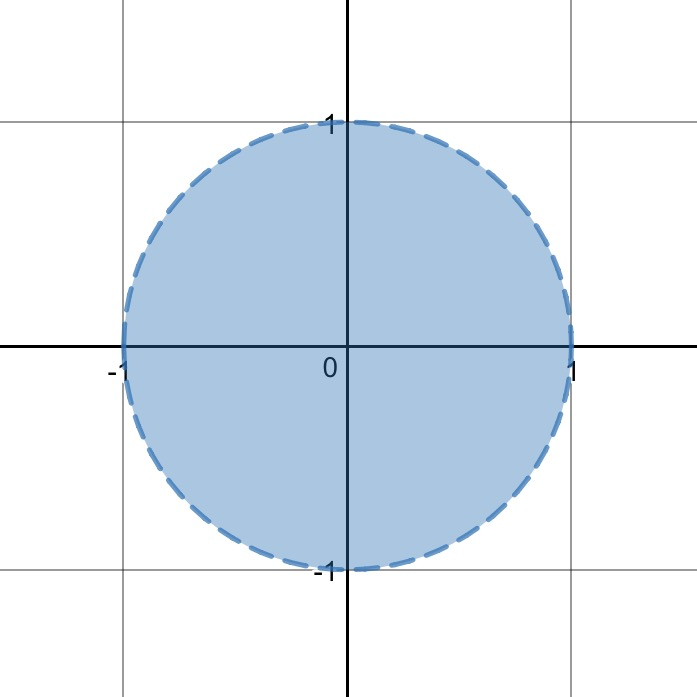
\includegraphics[scale=.125]{450b_hw3_prob4b_0}
%\caption{The set $U$ in $\R^2$}
%\end{figure}

Now, under $f$, every ordered pair maps either to itself, or to a corresponding ordered pair in the first quadrant (or on its boundary); so the image of $U$ is $f(U)=U\cap I$, where $I$ denotes the closure of the first quadrant.

\jpg{scale=.125}{adv_calc_ii_homework/450b_hw3_prob4b_1}

%\begin{figure}[h]
%\centering
%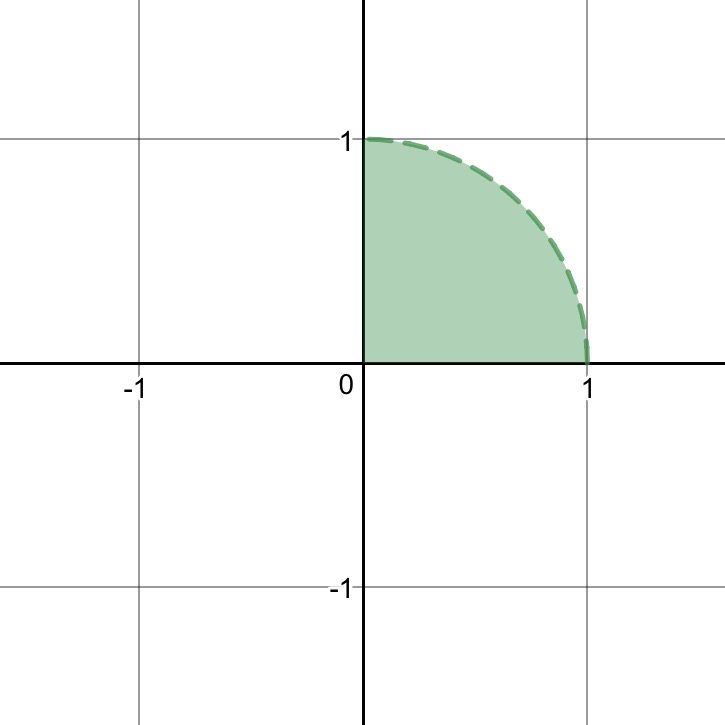
\includegraphics[scale=.125]{450b_hw3_prob4b_1}
%\caption{The set $f(U)$ in $\R^2$}
%\end{figure}

The set $f(U)$ is not open; since the origin $\vecb{0} \in f(U)$, but every $B(\vecb{0},r)$ contains points in every quadrant, so no open ball $B(\vecb{0},r)$ is a subset of $f(U)$.

\jpg{scale=.125}{adv_calc_ii_homework/450b_hw3_prob4b_2}

%\begin{figure}[h]
%\centering
%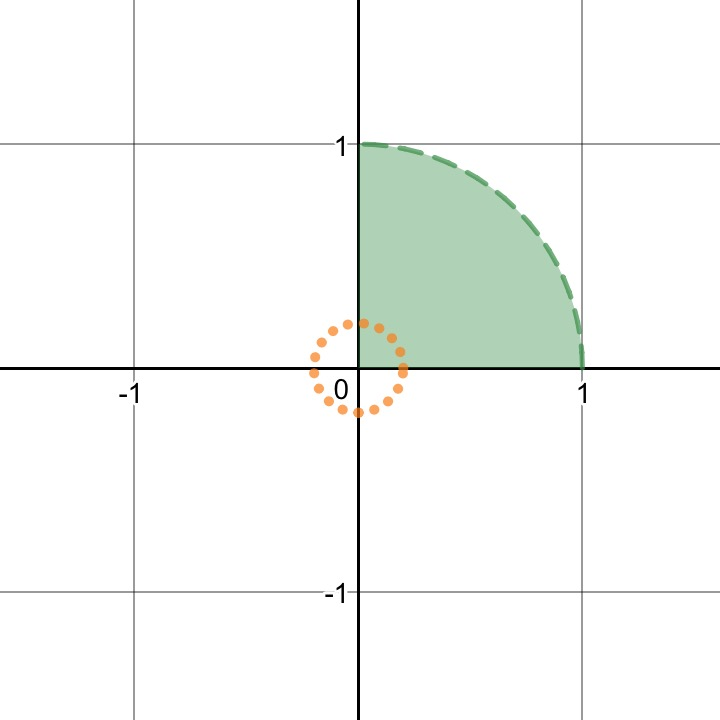
\includegraphics[scale=.125]{450b_hw3_prob4b_2}
%\caption{Every $B(\vec{0},r) \not\subset f(U)$}
%\end{figure}

Therefore, (2) fails. Thus, (1) $\centernot\implies$ (2). 
\end{proof}
\end{example*}

%6
\item Suppose that  $f:A\subset \R^n\to \R$ is continuous, with $\vecb{a}\in A$ and $f(\vecb{a})>0$. Prove that there exists a $\delta>0$ such that $f(\vecb{x})>0$ for all $\vecb{x}\in B(\vecb{a},\delta)\cap A$. 
\begin{proof}
Since $f$ is continuous on $A$, for every $\epsilon>0$, there exists a $\delta>0$ such that if $\norm{\vecb{x}-\vecb{a}}<\delta$ and $\vecb{x}\in A$, then $\norm{f(\vecb{x})-f(\vecb{a})}<\epsilon$. Let $\epsilon=f(\vecb{a})$. If $\norm{f(\vecb{x})-f(\vecb{a})}<f(\vecb{a})$, then $f(\vecb{x})\in B(f(\vecb{a}), f(\vecb{a}))$, which is the interval $(0, 2f(\vecb{a}))$. Thus, we are done.
\end{proof}

%7
\item Suppose that $A \subset \R^n$ is a set which is not closed. Prove that there exists a continuous function $f:A\to\R$ which is unbounded. (Hint: You might find it useful to first show that the set $\R^n-A$ must contain a point in the boundary of $A$.)
\begin{lemma*}[7.1]
If a set $A$ contains all its boundary points, then it is closed. 
\end{lemma*}
\begin{proof}
$A$ contains all of its boundary points, so $A^\complement$ contains none of them. That is, for all $\vecb{x}\in A^\complement$, $\vecb{x}$ is not a boundary point, so there exists some $r>0$ such that $B(\vecb{x}, r)\subset A^\complement$. This means that $A^\complement$ is open, by the openness criterion. Furthermore, since $A^\complement$ is open, $A$ is closed. 
\end{proof}
By the way, we have also proved the following:
\begin{corollary*}[7.2]
If a set $A$ contains none its boundary points, then it is open.
\end{corollary*}
Okay, now we are ready to prove Exercise 7. 
\begin{proof}
Suppose that $A \subset \R^n$ is not closed. By the contrapositive of Lemma (7.1), $A$ does not contain all of its boundary points. Let $\vecb{p}$ be a boundary point of $A$ which is not in $A$. Now, let $f:A\to\R$ be defined as 
$$f(\vecb{x})=\frac{1}{\norm{\vecb{x}-\vecb{p}}}.$$
To see that $f$ is unbounded, observe that for any $B>0$, $B(\vecb{p},\frac{1}{B})$ contains a point in $A$, so there exists some $\vecb{a}\in B(\vecb{p},\frac{1}{B})$ such that $\norm{\vecb{a}-\vecb{p}}<\frac{1}{B}$, so $f(\vecb{x})=\frac{1}{\norm{\vecb{a}-\vecb{p}}}>B$. 
\end{proof}
\end{enumerate}


\pagebreak
\section{Index}
\printindex

\end{document}

